\chapter{Modelos de difusión}
\label{dm}

En este capítulo se definirán y estudiarán los modelos generativos de difusión, los cuales constituyen el estado del arte en la generación de imágenes. Estos modelos distorsionan progresivamente los datos de entrenamiento provenientes desde una distribución de probabilidad $\ptrue$ hasta llegar a una distribución final $\pprior$. Resolviendo un problema de optimización para aprender las transiciones del proceso reverso, es posible generar nuevas muestras desde $\ptrue$ a partir de una muestra generada desde $\pprior$ mediante la simulación del proceso backward aprendido.

Dado que los modelos de difusión han sido investigados principalmente desde un punto de vista práctico, en este primer capítulo se asumirá, como es usual en el aprendizaje automático, que la medida de probabilidad que genera los datos de entrenamiento posee una función de densidad $\ptrue$\footnote{Es decir, se asumirá que la medida que genera los datos es absolutamente continua con respecto a la medida de Lebesgue en $\R^d$ (ver \autoref{defn:absolute_continuity_measures}), cuya consecuencia más importante es, de acuerdo al teorema de Radon-Nikodym (ver \autoref{teo:radon_nikodym}), que existe una función de densidad y esta es única.}. Esta suposición se levantará en los capítulos posteriores, donde se trabajará directamente sobre medidas de probabilidad.

\section{Modelos generativos neuronales}
\label{dm/generative_models}

A modo de introducción, se explorarán dos enfoques fundamentales en el campo de los modelos generativos neuronales: las redes generativas adversarias (GANs) y los modelos basados en energía (EBMs). Estos modelos representan diferentes paradigmas para abordar el desafío de generar muestras que se asemejen a una distribución empírica que representa observaciones disponibles. Por un lado, las GANs han revolucionado el campo de la generación de imágenes mediante un enfoque de competencia entre dos redes neuronales, mientras que los EBMs ofrecen una perspectiva alternativa, modelando explícitamente la densidad de probabilidad de los datos a través de una función de energía. Como se verá a lo largo de la sección, ambos enfoques tienen sus propias fortalezas y limitaciones, y su estudio permitirá apreciar cómo los modelos de difusión abordan algunas de las limitaciones de estos enfoques más clásicos.

Por otra parte, en la \autoref{dm/continuous_dm/score} se verá una estrecha conexión entre los modelos de difusón y los EBMs.

\subsection{Redes generativas adversarias}
\label{dm/generative_models/gans}

Previo al uso de modelos de difusión, las redes generativas adversarias\footnote{También se les conoce como redes generativas adversativas o antagónicas.} (GANs) constituyeron durante varios años el estado del arte de los modelos generativos para imágenes. Este tipo de modelos fueron propuestos por investigadores de la Universidad de Montreal en \cite{goodfellow2014generative}, donde los autores propusieron entrenar dos modelos independientes representados por redes neuronales. Por un lado, un modelo generador $G$ busca aprender a generar muestras artificiales a partir de una cierta distribución $\ptrue$, engañando a otro modelo discriminador $D$ que busca discernir si una muestra de entrada corresponde a una muestra proveniente de $\ptrue$ o a una muestra artificial generada por $G$.

\subsubsection{Formulación y convergencia}

La descripción anterior afirma que el modelo generativo que propone una GAN consta de dos partes:

\begin{itemize}
	\item $G_\theta$ es un modelo generativo de variable latente que transforma una distribución latente $z\sim p_z(z)$ en otra distribución $g\sim p_g(g)$ mediante $z\mapsto G_\theta(z)$. El objetivo de este modelo es que $p_g\approx\ptrue$, por lo que puede ser comparado con el decoder de un autoencoder variacional (ver \autoref{dm/vae}).
	\item $D_\phi$ es un modelo discriminativo probabilístico (clasificador) tal que, para una cierta entrada $x$, $D_\phi(x)$ indica la probabilidad de que $x$ provenga de la distribución real de los datos. Es decir, si una muestra $x$ proviene de $\ptrue$ entonces $D_\phi(x)=1$ mientras que si proviene de $p_g$, entonces $D_\phi(x)=0$. \end{itemize}

Con esto, se tiene una única función objetivo para ambos modelos, la cual está asociada al rendimiento del modelo discriminador. Por un lado, $D$ busca maximizar su capacidad de predicción, mientras que $G$ busca minimizarla:

\begin{equation}
    \label{eq:gan_objective}
	\min_\theta\max_\phi C(G_\theta, D_\phi) := \E{x\sim\ptrue(x)}{\log D_\phi(x)} + \E{z\sim p_z(z)}{\log (1-D_\phi(G_\theta(z)))}.
\end{equation}

Los modelos $G_\theta$ y $D_\phi$ se entrenan de forma alternada, comenzando por el discriminador. Además, por motivos teóricos que se verán a continuación, el discriminador se suele entrenar $K\geq 1$ veces por cada iteración del generador (es decir, por cada iteración del descenso del gradiente sobre el generador, el discriminador realiza $K$ iteraciones de descenso del gradiente). El bucle de entrenamiento para una GAN genérica puede ser encontrado en el \autoref{alg:gan_training}, donde las esperanzas son estimadas por aproximaciones de por Monte Carlo. Una ilustración de su dinámica se puede encontrar en la \autoref{fig:dm/gan_training}.

\begin{algorithm}
	\caption{Entrenamiento de una GAN}
    \label{alg:gan_training}
	\begin{algorithmic}[1]
		\Require número de pasos $K$ para entrenar el discriminador, redes neuronales $G_\theta$ y $D_\phi$.
		\While{no hay convergencia}
		\For{$k = 1$ to $K$}
		\State Obtener batch de entrenamiento $\{x_1,\ldots,x_m\}$ con $x_i\sim\ptrue(x_i)$, $\forall i\in\{1,\ldots,m\}$.
		\State Generar batch de latentes $\{z_1,\ldots,z_m\}$ con $z_i\sim p_z(z_i)$, $\forall i\in\{1,\ldots,m\}$.
		\State Realizar un paso del algoritmo de gradiente ascendente para el discriminador mediante el gradiente

		\begin{equation*}
			\nabla_\phi \frac{1}{m}\sum_{i=1}^m \left(\log D_\phi(x_i) + \log(1-D_\phi(G_\theta(z_i)))\right)
		\end{equation*}

		\EndFor
		\State Generar batch de latentes $\{z_1,\ldots,z_m\}$ con $z_i\sim p_z(z_i)$, $\forall i\in\{1,\ldots,m\}$.
		\State Realizar un paso del algoritmo de gradiente descendente para el generador mediante el gradiente

		\begin{equation*}
			\nabla_\theta \frac{1}{m}\sum_{i=1}^m \left( \log(1-D_\phi(G_\theta(z_i)))\right)
		\end{equation*}

		\EndWhile
	\end{algorithmic}
\end{algorithm}

\insertimage{dm/gan_training}{0.8}{Dinámica de entrenamiento de una GAN. La curva negra segmentada representa a $\ptrue$, la curva verde representa $p_g$ y la línea azul segmentada representa la distribución aprendida por el discriminador. En (a) se tiene el estado actual de la GAN luego de algunas iteraciones donde la convergencia del discriminador aún no es alcanzada. En (b) se observa el estado de la GAN luego de entrenar el clasificador. En (c) se ve el el estado de la GAN luego de optimizar el generador. En (d) se observa la convergencia, donde $p_g$ es indistinguible de $\ptrue$ y el discriminador sigue una distribución de Bernoulli (máxima entropía). Imagen obtenida desde \cite{goodfellow2014generative}.}

En la \autoref{fig:dm/gan_samples} se pueden observar imágenes generadas a partir de una GAN sobre los dataset MNIST y FashionMNIST utilizando una red fully-connected y el algoritmo de entrenamiento indicado en el \autoref{alg:gan_training}.

\begin{figure}
    \centering
    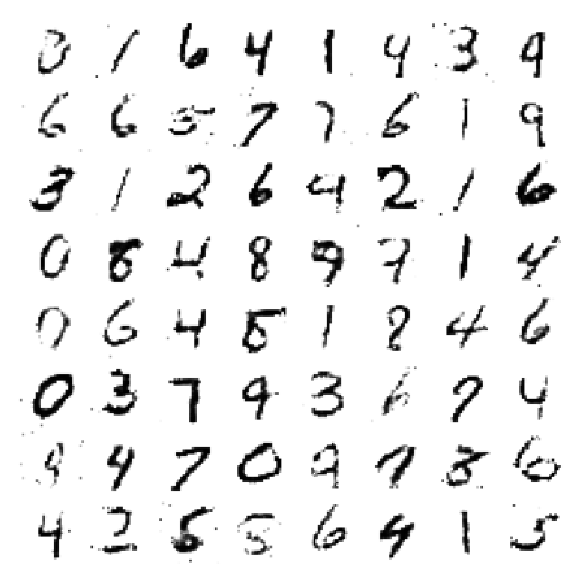
\includegraphics[width=0.45\textwidth]{images/dm/gan_mnist}
    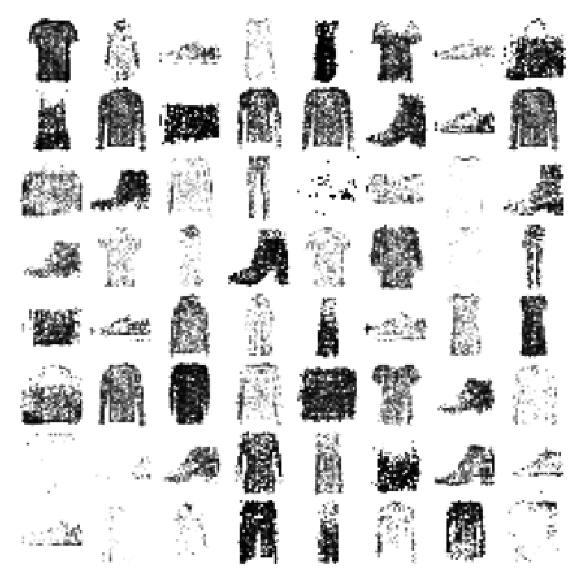
\includegraphics[width=0.45\textwidth]{images/dm/gan_fashion_mnist}
    \caption{Imágenes generadas por una GAN entrenada durante 50 épocas con una red fully-connected sobre el dataset MNIST (izquierda) y FashionMNIST (derecha). La implementación de este modelo se encuentra en el archivo \texttt{gan\_images.ipynb}. En el archivo \texttt{gan.ipynb} se puede encontrar una implementación para datos bidimensionales.}
    \label{fig:dm/gan_samples}
\end{figure}

Por otra parte, los autores de \cite{goodfellow2014generative} muestran algunos resultados elementales acerca de la convergencia de las GANs. El primero de ellos afirma que, dado un generador fijo $G$, el discriminador óptimo tiene el comportamiento esperado:

\begin{prop}[discriminador óptimo]
	Para un generador $G$ fijo, el discriminador óptimo $D^*_G$ viene dado por:

	\begin{equation*}
		D^*_G(x) = \frac{\ptrue(x)}{\ptrue(x) + p_g(x)}.
	\end{equation*}
\end{prop}

Por otra parte, asumiendo que siempre es posible obtener un discriminador óptimo $D_G^*$ para un generador $G$, el siguiente resultado afirma que el generador óptimo para \eqref{eq:gan_objective} se alcanza cuando $p_g=\ptrue$:

\begin{prop}[generador óptimo]
	Para una función objetivo $C(G):=C(G, D_G^*) = \max_\phi C(G, D_\phi)$, su mínimo global $G^*=\argmin_\theta C(G_\theta)$ es alcanzado si y solo si $p_g=\ptrue$. En este caso, $C(G^*)=-\log 4$.
\end{prop}

Estos resultados permiten concluir que al seguir el algoritmo dado en el \autoref{alg:gan_training}, la distribución $p_g$ asociada al generador converge a $\ptrue$:

\begin{prop}[convergencia del \autoref{alg:gan_training}]
	Si los modelos $G_\theta$ y $D_\phi$ tienen suficiente capacidad y $K$ es lo suficientemente grande como para permitir que $D_\phi$ sea óptimo en cada iteración, entonces $p_g$ converge a $\ptrue$.
\end{prop}

En la proposición anterior, es importante entrenar el discriminador hasta su convergencia, lo cual justifica la asimetría dada en el \autoref{alg:gan_training}.

\subsubsection{Generación condicional}

El modelo descrito anteriormente es un modelo generativo que busca aprender la distribución no condicional $\ptrue$, por lo que no es posible controlar la generación. En \cite{mirza2014conditional} los autores proponen realizar un pequeño cambio a la arquitectura para  permitir generar muestras a partir de una distribución condicional $\ptrue(x|y)$, donde $y$ es una etiqueta o condición sobre los datos. Esto permite, por ejemplo, generar dígitos específicos con la GAN usada para la \autoref{fig:dm/gan_samples}.

Para conseguir esto, solo hace falta modificar la estructura de los modelos $G_\theta$ y $D_\phi$ para permitir una entrada adicional $y$. Con esto, la nueva función objetivo es

\begin{equation*}
	\min_\theta\max_\phi C(G_\theta, D_\phi) := \E{(x,y)\sim\ptrue(x,y)}{\log D_\phi(x|y)} + \E{z\sim p_z(z),y\sim \ptrue(y)}{\log (1-D_\phi(G(z|y)))}.
\end{equation*}

\subsubsection{Limitaciones de las GANs}

Uno de los problemas más conocidos en las GANs es que poseen un entrenamiento altamente inestable, dependiendo fuertemente de la arquitectura, hiperparámetros y datos utilizados durante el entrenamiento. Con el fin de aminorar la inestabilidad provocada por la arquitectura, los autores de \cite{radford2016unsupervised} proponen algunas reglas generales para la construcción de una arquitectura para GANs, denominada DCGAN (deep convolutional GAN). En particular, concluyen lo siguiente:

\begin{itemize}
	\item Las capas de global average pooling estabilizan el entrenamiento pero la convergencia se vuelve más lenta. Debido a esto, proponen sustituir las capas de pooling por capas convolucionales con stride en el encoder y por capas convolucionales transpuestas con stride fraccional en el generador.
	\item Usar batch normalization \cite{ioffe2015batch} tanto en el generador como en el discriminador. Si bien hoy en día esto es una práctica frecuente, no era obvio su uso en la fecha de publicación de este trabajo.
	\item Eliminar capas fully-connected en arquitecturas profundas.
	\item Usar ReLU en el generador (excepto en la última capa donde se suele usar $\tanh$) y Leaky-ReLU en el discriminador.
\end{itemize}

Por otra parte, un problema intrínseco de este tipo de modelos es que tienden a concentrar su aprendizaje en las modas de las distribuciones, perdiendo la capacidad de generar muestras más diversas. Si bien este problema no es notorio en datasets de juguete como MNIST, sí se vuelve importante cuando se busca aprender distribuciones más complejas, donde es usual tener que entrenar una GAN para cada grupo de datos de la distribución. Como se verá en la \autoref{dm/discrete_dm}, los modelos de difusión no poseen este problema, pudiendo aprender distribuciones complejas y generar muestras de alta calidad.

\subsection{Modelos basados en energía}
\label{dm/generative_models/ebm}

Los modelos basados en energía (EBMs) constituyen otra familia importante de modelos generativos neuronales. A diferencia de las GANs, que aprenden implícitamente la distribución de los datos a través de una dinámica adversativa, los EBMs aprenden explícitamente una función de energía que caracteriza la distribución de probabilidad de los datos.

Un EBM busca aproximar una distribución de probabilidad $\ptrue$ mediante otra distribución $p_\theta(x)$ parametrizada por $\theta$ de la siguiente forma:

\begin{equation}
    \label{eq:energy_density}
    p_\theta(x) = \frac{1}{Z(\theta)} \exp(-E_\theta(x)),
\end{equation}

donde $E_\theta: \mathbb{R}^d \to \mathbb{R}$ se denomina \textit{función de energía} y $Z(\theta) = \int_{\mathbb{R}^d} \exp(-E_\theta(x)) \d x$ es la constante de normalización, también conocida como \textit{función de partición}. El nombre de este tipo de modelos viene de su interpretación física, donde \eqref{eq:energy_density} corresponde a una parametrización de la distribución de Boltzmann, la cual será definida posteriormente en \eqref{eq:boltzmann}.

La función de energía $E_\theta$ es típicamente modelada por una red neuronal, lo que permite capturar relaciones complejas entre los datos y heredar sus propiedades de diferenciabilidad. Para el entrenamiento de este tipo de modelos, se busca ajustar los parámetros de $E_\theta(x)$ para que la distribución aprendida, $p_\theta(x)$, se aproxime a la verdadera distribución de los datos, $\ptrue$. Para esto, es usual minimizar la divergencia de Kullback-Leibler entre $\ptrue$ y $p_\theta$:

\begin{defn}[divergencia de Kullback-Leibler, caso absolutamente continuo]
    \label{defn:kl_ac}
    Dadas dos densidades de probabilidad $p$ y $q$ en $\R^d$, se define la divergencia de Kullback-Leibler entre $p$ y $q$ como\footnote{Notar que la integral de abajo solo está bien definida si $p(x)=0$ cuando $q(x)=0$, es decir, si $p\ll q$ (en el sentido de las medidas que inducen estas densidades). A diferencia de la continuidad absoluta asumida para la existencia de las densidades, esta restricción es propia de la divergencia de Kullback-Leibler.}:


    \begin{equation*}
        \KL{p}{q}
        = \E{p(x)}{\log \frac{p(x)}{q(x)}}
        = \int_{\R^d} \log\parent{\frac{p(x)}{q(x)}}p(x) \d x,
    \end{equation*}

    donde se define, por continuidad, $0\cdot\log(0)=0$ en los casos que sea necesario.
\end{defn}

Es importante recordar que a lo largo de este capítulo se asumirá siempre la existencia de densidades de probabilidad, por lo que la divergencia de Kullback-Leibler se puede definir mediante la expresión dada en la \autoref{defn:kl_ac}. Sin embargo, en el \autoref{ot} y en el \autoref{eot_sbp} será necesario trabajar directamente sobre medidas de probabilidad, donde la existencia de tales densidades no está garantizada. Esto exigirá redefinir la divergencia de Kullback-Leibler en función de la derivada de Radon-Nikodym (ver \autoref{teo:radon_nikodym}).

Con esta definición, el parámetro óptimo para un EBM es el que minimiza la siguiente divergencia:

\begin{equation*}
    \theta^* = \argmin_\theta \KL{p_{\text{true}}}{p_\theta}.
\end{equation*}

Notar que esta es una cantidad conveniente de minimizar para un modelo de energía ya que al desarrollar esta expresión, se llega a que minimizar la divergencia de Kullback-Leibler es equivalente a maximizar la log-verosimilitud de los datos, lo cual se puede escribir directamente en función de la función de energía:

\begin{equation*}
    \KL{p_{\text{true}}}{p_\theta}
    = \E{x \sim p_{\text{true}}}{\log\frac{\ptrue(x)}{p_\theta(x)}}
    = \E{x \sim p_{\text{true}}}{\log \ptrue(x)} + \E{x \sim p_{\text{true}}}{-E_\theta(x)} + \log Z(\theta).
\end{equation*}

Sin embargo, el cálculo exacto de $\log Z(\theta)$ es intratable en la mayoría de los casos prácticos, ya que implica una integral sobre todo el espacio de datos. Si bien se han propuesto métodos para un entrenamiento aproximado de este modelo, en la \autoref{dm/continuous_dm/score} se verá una variante de esta familia de modelos donde se aprenderá directamente $\score{x}{p_\theta(x)}$ en vez de la función de energía.

Por último, para la generación de muestras a partir de un modelo de energía entrenado, $E_\theta$, es usual utilizar un algoritmo de sampling denominado \textit{Langevin sampling}, el cual requiere computar $\nabla_x E_\theta$. Este algoritmo está detallado en el \autoref{alg:langevin}, donde es usado para generar muestras a partir de un modelo basado en \textit{score}.

Debido a que el algoritmo de Langevin sampling consiste en simular una cadena de Markov, el tiempo de simulación es mucho más lento que en una GAN. Además, este tipo de modelos también sufre de inestabilidades durante el entrenamiento. En \cite{song2021trainenergybasedmodels} estudian en detalle este tipo de modelos junto a diversas técnicas de entrenamiento y muestran su relación con los modelos de \textit{score matching} estudiados en la \autoref{dm/continuous_dm/score}.

Las limitaciones mencionadas han motivado la investigación de enfoques generativos alternativos como los autoencoders variacionales (VAEs), que abordan algunas de estas limitaciones ofreciendo un entrenamiento más estable, una generación de muestras más rápida y una forma explícita de aproximar la verosimilitud.

\section{Autoencoders variacionales}
\label{dm/vae}

Con el fin de introducir el estudio de los modelos de difusión, se comenzará estudiando una familia de modelos generativos denominada autoencoders variacionales, los cuales permitirán obtener una construcción natural de los modelos de difusión en la \autoref{dm/discrete_dm}. Además, hoy en día es usual trabajar con ambos modelos de manera conjunta, donde un autoencoder variacional actúa como un reductor de dimensionalidad para así poder trabajar con los modelos de difusión sobre un espacio latente (ver \autoref{dm/discrete_dm/improvements}).

\subsection{Modelos de variable latente}
\label{dm/vae/latent_models}

Un enfoque frecuente en formulación de modelos generativos es el uso de variables latentes. Este tipo de modelos propone que los datos observados a partir de $x\sim\ptrue$ provienen realmente\footnote{Si bien esto no tiene por qué ser cierto, se puede asumir sin pérdida de generalidad, ya una posible independencia entre $x$ y $z$ vuelve prescindible a la variable latente $z$.} de una distribución conjunta con densidad $\ptrue(x,z)$, donde la componente $z$ es una variable aleatoria latente (i.e., no es observada) que influye directamente en la generación de las muestras observadas (componente $x$). Con esto, los modelos de variable latente proponen un modelo gráfico cuyas densidad se factoriza como

\begin{equation}
    \label{eq:latent_model}
    p_\theta(x,z)=p_\theta(z)p_\theta(x|z).
\end{equation}

Además, es usual suponer que la dimensión de la variable latente $z$ es estrictamente menor que la dimensión de los datos observados $x$. A lo largo de este capítulo, se considerará siempre que los datos observados viven en el espacio ambiente $\R^d$, mientras que las características ocultas estarán inmersas en el espacio $\R^l$, con $l\ll d$. Esta elección permite muchas veces transformar datos de alta dimensión a representaciones de menor dimensión, pudiendo ganar eficiencia computacional sin perder una cantidad significativa de información. Esto último se suele justificar mediante el siguiente resultado, el cual afirma que es posible proyectar un conjunto de $n$ puntos en $\R^d$ a cualquier espacio de dimensión mayor o igual a $\mathcal{O}\parent{\frac{\log n}{\epsilon^2}}$ de tal forma que la distancia euclidiana original de los puntos no se distorsione más allá de un factor $1\pm\epsilon$. Además, el mapa de proyección puede ser encontrado aleatoriamente en tiempo polinomial (en el sentido de Turing), aunque para efectos de los modelos generativos, este último resultado es omitido ya que se suele buscar un proyector mediante el entrenamiento de una red neuronal:

\begin{teo}[Johnson-Lindenstrauss]
    Sea $\epsilon\in (0,1)$ y $\{x^k\}_{k=1}^n\subset\R^d$ un conjunto de puntos. Entonces, para todo $l\in\N$ con $l\geq\frac{24}{3\epsilon^2 - 2\epsilon^3} \log n$, existe un mapa $f:\R^d\to\R^l$ tal que

    \begin{equation*}
        (1-\epsilon)\norm{x_i-x_j}^2 \leq \norm{f(x_i)-f(x_j)}^2 \leq (1+\epsilon)\norm{x_i-x_j}^2, \quad\forall i,j\in\{1,\ldots,n\}.
    \end{equation*}

    Además, existe un conjunto $\{x^k\}_{k=1}^n\subset\R^d$ tal que la cota para $l\in\N$ es alcanzada. En cualquier caso, el problema de encontrar $f$ está en la clase de complejidad $\operatorname{BPP}$\footnote{Recordar que esta es la clase de problemas decidibles en tiempo polinomial por máquinas de Turing probabilísticas con una probabilidad de error menor a $\frac{1}{3}$ (ver \cite{arora2009computational}).}.
\end{teo}

Una demostración de este resultado se puede encontrar en \cite{dasgupta2003elementary}.

\subsubsection{Criterio de máxima verosimilitud}

Un criterio natural para elegir un mejor modelo dentro de una familia de modelos generativos es el criterio de máxima verosimilitud. En \cite{nichol2021improved} afirman que hoy en día se cree que optimizar un modelo generativo maximizando la log-verosimilitud, fuerza al modelo a capturar todas las modas de la distribución de los datos de entrenamiento, lo cual no ocurre al entrenar una GAN.

\begin{defn}[función de log-verosimilitud]
    Sea $\mathcal{V}=\{p_\theta\}_{\theta\in\Theta}$ una familia paramétrica de funciones de densidad de probabilidad y $\mathcal{D} = \{x^k\}_{k=1}^n\subset\R^d$ un conjunto de observaciones\footnote{En este trabajo se utilizará la notación de superíndice para indexar un conjunto de muestras, reservando la notación de sub-índice para una familia de variables aleatorias.} i.i.d. provenientes de alguna distribución desconocida $\ptrue$. La función de log-verosimilitud $l:\Theta\to\R$ asociada a $\mathcal{V}$ y a $\mathcal{D}$ se define como:

    \begin{equation*}
        l_\mathcal{V}\parent{\theta|\mathcal{D}}
        := \sum_{k=1}^n \log p_\theta(x^k).
    \end{equation*}
\end{defn}

Con esta definición, el criterio de máxima verosimilitud elige, como su nombre lo indica, al modelo generativo que maximiza la (log-)verosimilitud dentro de la familia de modelos:

\begin{equation*}
    \theta_{\text{MLE}}
    =\argmax_{\theta\in\Theta} l_\mathcal{V}\left(\theta|\mathcal{D}\right).
\end{equation*}

Sin embargo, para utilizar el criterio de máxima verosimilitud es necesario poder evaluar la log-densidad marginal $\log p_\theta(x)$ en el conjunto de datos de entrenamiento (de aquí en adelante, a esta cantidad se le denominará \textit{evidencia}). En un modelo de variable latente factorizado como $p_\theta(x,z)=p_\theta(z)p_\theta(x|z)$ en general no es posible dicha evaluación, en efecto:

\begin{equation}
    \label{eq:generative_marginal}
    p_\theta(x)
    = \int_{\R^l} p_\theta(x,z) \d z
    = \frac{p_\theta(z)p_\theta(x|z)}{p_\theta(z|x)}.
\end{equation}

La primera igualdad corresponde a la marginalización de $x$, mientras que la segunda igualdad se obtiene al aplicar la definición de probabilidad condicional, $p_\theta(x,z)=p_\theta(x)p_\theta(z|x)$. Notar que la primera igualdad no es tratable para modelos $p_\theta$ complejos ya que requiere evaluar varias veces el modelo para aproximar la integral numéricamente. La segunda igualdad no es computable dado que no se conoce la posterior $p_\theta(z|x)$ debido a que $z$ es una variable oculta.

\subsubsection{Cota inferior de la evidencia}

Debido a que no es posible calcular explícitamente la evidencia de un modelo de variable latente, se utilizará un enfoque aproximado para su evaluación, el cual está basado en técnicas de inferencia variacional (ver, por ejemplo, \cite{Blei_2017}). En este caso, la densidad marginal $p_\theta(x)$ será calculada utilizando la segunda igualdad en \eqref{eq:generative_marginal}, donde la posterior $p_\theta(z|x)$ se aproximará mediante un nuevo modelo paramétrico $q_\phi(z|x)$, el cual se puede interpretar como un modelo generativo condicional para la variable latente.

Si bien se podría sustituir directamente el nuevo modelo $q_\phi(z|x)$ en \eqref{eq:generative_marginal} y obtener $p_\theta(x)\approx\frac{p_\theta(z)p_\theta(x|z)}{q_\phi(z|x)}$, no es posible maximizar dicha cantidad de forma conjunta ya que, al no tener una restricción que asegure que $q_\phi(z|x)$ aproxime a $p_\theta(z|x)$, bastaría tomar $p_\theta(x,z)\to\infty$ y $q_\phi(z|x)\to 0^+$ para la maximización. Debido a esto, se utilizará, como es usual en el aprendizaje automático, la divergencia de Kullback-Leibler (ver \autoref{defn:kl_ac}) para comparar la densidad $q_\phi(z|x)$ con la densidad que realmente busca estimar, $p_\theta(z|x)$:

\begin{equation*}
    \KL{q_\phi(z|x)}{p_\theta(z|x)}
    = \E{q_\phi(z|x)}{\log\frac{q_\phi(z|x)}{p_\theta(z|x)}}
    = \E{q_\phi(z|x)}{\log\frac{q_\phi(z|x)}{p_\theta(x,z)} + \log p_\theta(x)},
\end{equation*}

de donde se obtiene una relación explícita entre el error de aproximación de $q_\phi(z|x)$ y la evidencia:

\begin{prop}[descomposición de la evidencia]
    Dado un modelo paramétrico auxiliar $q_\phi(z|x)$ para la distribución posterior $p_\theta(z|x)$, se tiene la siguiente descomposición para la evidencia:

    \begin{equation}
        \label{eq:evidence_decomposition}
        \log p_\theta(x)
        = \KL{q_\phi(z|x)}{p_\theta(z|x)} + \underbrace{\E{q_\phi(z|x)}{\log\frac{p_\theta(x,z)}{q_\phi(z|x)}}}_{\elbo}.
    \end{equation}
\end{prop}

Si bien el primer término de la igualdad no es tratable ya que requiere conocer la posterior verdadera, $p_\theta(z|x)$, la desigualdad de Gibbs\footnote{Esta desigualdad afirma que la divergencia de Kullback-Leibler es siempre no negativa.} permite afirmar que el término definido como ELBO\footnote{Notar que la ELBO depende de $x$, por lo que debería escribirse como $\elbo(x)$. A lo largo de este trabajo se escribirá, por simplicidad, simplemente $\elbo$, sin olvidar la dependencia en la variable observada $x$.} (\textit{evidence lower bound}) es una cota inferior de la evidencia $\log p_\theta(x)$. Además, esta descomposición sugiere que maximizar la ELBO es una función objetivo natural para abordar el problema de la máxima verosimilitud ya que

\begin{equation*}
    \elbo = \log p_\theta(x) - \KL{q_\phi(z|x)}{p_\theta(z|x)},
\end{equation*}

y, por lo tanto, al maximixar la ELBO según su definición en \eqref{eq:evidence_decomposition} se estará maximizando la evidencia al mismo tiempo que se minimiza la divergencia $\KL{q_\phi(z|x)}{p_\theta(z|x)}$. Además, el hecho de que la $\elbo$ sea una cota inferior de la evidencia, la maximización de la $\elbo$ se puede ver como el problema de optimizar el peor caso de la log-verosimilitud. De este modo, si los modelos $p_\theta$ y $q_\phi$ tienen suficiente capacidad, se estará optimizando la evidencia al mismo tiempo que se ajusta el modelo auxiliar $q_\phi(z|x)$ a la posterior real $p_\theta(z|x)$.

Por otra parte, si bien la definición de la ELBO dada en \eqref{eq:evidence_decomposition} es aproximable mediante estimaciones de Monte Carlo, su expresión es poco interpretable. Sin embargo, es posible trabajar más esta expresión:

\begin{equation*}
    \elbo
    = \E{q_\phi(z|x)}{\log\frac{p_\theta(z)p_\theta(x|z)}{q_\phi(z|x)}}
    = \E{q_\phi(z|x)}{\log p_\theta(x|z)} + \E{q_\phi(z|x)}{\log\frac{p_\theta(z)}{q_\phi(z|x)}}.
\end{equation*}

En consecuencia, viendo que el segundo término de la segunda igualdad corresponde (al negativo de) una divergencia de Kullback-Leibler, se llega a la caracterización usada en general:

\begin{prop}[descomposición de la ELBO]
    Se tiene la siguiente descomposición para la ELBO:

    \begin{equation}
        \label{eq:elbo_decomposition}
        \elbo
        = \underbrace{\E{q_\phi(z|x)}{\log p_\theta(x|z)}}_{\text{término de reconstrucción}}
        - \underbrace{\KL{q_\phi(z|x)}{p_\theta(z)}}_{\text{prior matching}}.
    \end{equation}
\end{prop}

El término de reconstrucción\footnote{Si bien este término tiene forma de entropía cruzada, no lo es ya que $p_\theta(x|\cdot)$ no es distribución de probabilidad.}, el cual se estima mediante aproximaciones de Monte Carlo, mide qué tan probable es, en esperanza, que la variable latente $z$ asociada a $x$ (según $q_\phi(z|x)$) genere realmente a $x$ (según $p_\theta(x|z)$). Por otra parte, el segundo término busca que la posterior aproximada $q_\phi(z|x)$ no se desvíe demasiado del prior original $p_\theta(z)$, actuando como un regularizador sobre el modelo. En la \autoref{dm/vae/formulation} se verá que, bajo ciertas elecciones de modelos, el segundo término puede tener forma cerrada.

Es importante notar que cuando el modelo $p_\theta(x|z)$ tiene demasiada capacidad, es posible que este pueda reconstruir los datos $x\sim\ptrue$ sin hacer uso de la variable latente (i.e., $x$ se vuelve independiente de $z$). Este fenómeno se denomina colapso de la posterior y, si bien se sigue logrando el objetivo de tener un modelo generativo para $x$, ya no es posible guiar la generación de acuerdo a elecciones específicas de $z$, lo cual es deseable, por ejemplo, para interpolar entre muestras (ver \autoref{fig:dm/vae_interpolation}). Una posible solución es agregar la restricción de que el término \textit{prior matching} sea mayor que un cierto valor $\delta$, tal como se propone en \cite{razavi2019preventing}.

\begin{figure}
    \centering
    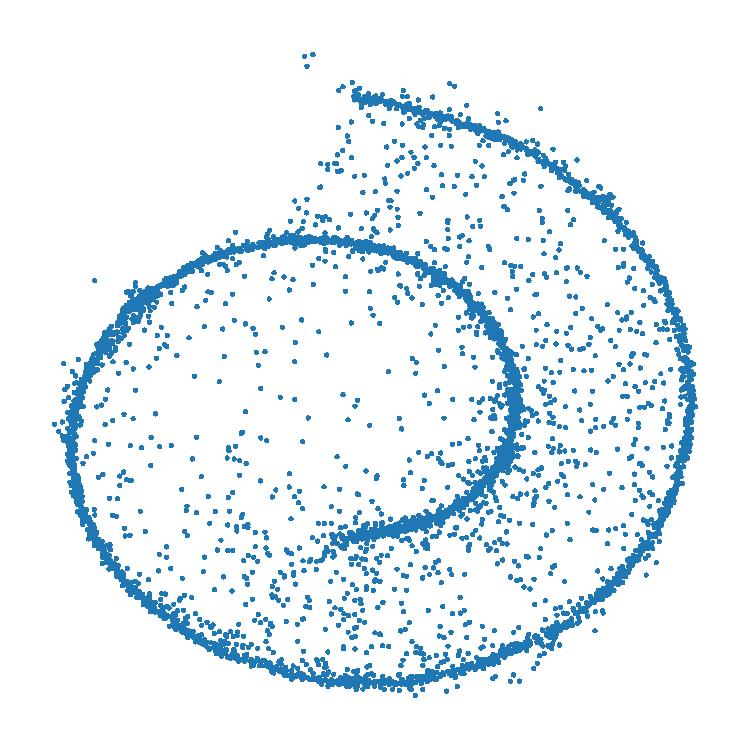
\includegraphics[width=0.3\textwidth]{images/dm/vae_samples_1d}
    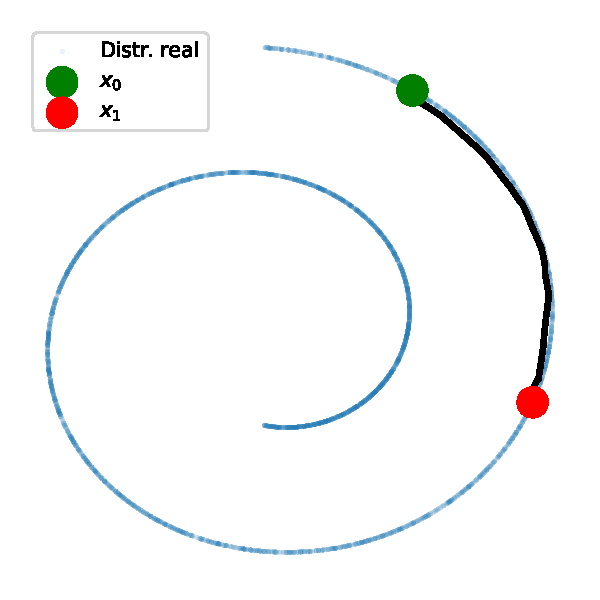
\includegraphics[width=0.3\textwidth]{images/dm/vae_interpolation_1d}
    \caption{(Izquierda) muestras generadas por un VAE para una distribución $\ptrue$ bidimensional. (Derecha) interpolación en el espacio latente del VAE, lo cual es posible debido a que no hay colapso de la posterior. La implementación de este modelo se encuentra en el archivo \texttt{vae\_1d.ipynb}.}
    \label{fig:dm/vae_interpolation}
\end{figure}

\paragraph{Conexión entre la ELBO y la física estadística}

De acuerdo a la física estadística, la probabilidad de que un sistema físico esté en un estado $k$ con energía $\varepsilon_k$ viene dada por la distribución de Boltzmann

\begin{equation}
	\label{eq:boltzmann}
	p(k) \propto \exp\left(-\frac{\varepsilon_k}{k_B T}\right),
\end{equation}

donde $k_B$ es la constante de Boltzmann y $T$ es la temperatura del sistema, por lo que la fracción en la función exponencial es adimensional.

Esto motiva a que el término $-\log p(k)$ sea generalmente llamado energía. Con esta analogía, es posible conectar la ELBO con la energía libre de Helmholtz. En efecto, al desarrollar la ELBO a partir de su definición original en \eqref{eq:evidence_decomposition}:

\begin{align*}
	\elbo &= \E{q_\phi(z|x)}{\log\frac{p_\theta(x,z)}{q_\phi(z|x)}}\\
    & = \E{q_\phi(z|x)}{\log p_\theta(x,z)} - \E{q_\phi(z|x)}{\log q_\phi(z|x)} \\
	& = -\underbrace{\E{q_\phi(z|x)}{-\log p_\theta(x,z)}}_{\text{energía esperada}} + \underbrace{\entropy{q_\phi(\cdot|x)}}_{\text{entropía}},
\end{align*}

donde $\entropy{\cdot}$ es el operador de entropía (ver \autoref{defn:discrete_entropy} para el caso discreto). Por otra parte, si $U$ es la energía interna de un sistema físico, $T$ es la temperatura ambiente y $S$ es la entropía del sistema, la energía libre de Helmholtz queda definida como:

\begin{equation*}
	F = U-TS,
\end{equation*}

la cual es, de acuerdo a la física estadística, minimizada en el equilibro termodinámico. En consecuencia, a la ELBO (la cual se busca maximizar) también se le conoce como energía libre variacional negativa.

En la \autoref{eot_sbp/static_sbp} se volverá a utilizar la distribución de Boltzmann para conectar el problema de regularización entrópica estudiado en la \autoref{eot_sbp/regularized} con el problema del puente de Schrödinger en su versión estática.

\subsection{Formulación de un VAE}
\label{dm/vae/formulation}

La descomposición de la ELBO dada en \eqref{eq:elbo_decomposition} motiva a elegir ciertos modelos $q_\phi(z|x)$ y $p_\theta(z)$ de tal forma que la divergencia $\KL{q_\phi(z|x)}{p_\theta(z)}$ tenga forma cerrada. Un autoencoder variacional (VAE) es un modelo de variable latente propuesto en \cite{kingma2022autoencoding} que propone la siguiente estructura para los modelos paramétricos:

\begin{align}
    q_\phi(z|x) & \sim \gaussian{\mu_\phi(x)}{\Sigma_\phi(x)} \label{eq:vae_model_posterior} \\
    p_\theta(z) & = p(z) \sim \gaussian{0}{\identity{l}} \label{eq:vae_model_prior},
\end{align}

donde $\mu_\phi:\R^d\to\R^l$ y $\Sigma_\phi:\R^d\to\mathcal{S}_l^{++}$\footnote{En este caso, $\mathcal{S}_l^{++}$ denota el conjunto de matrices de tamaño $l\times l$ que son simétricas y definidas positivas.} son funciones generalmente aprendidas por redes neuronales. Por otro lado, el modelo $p_\theta(x|z)$ (cuyos parámetros también serán aprendidos por una red neuronal) dependerá de la naturaleza de $x\in\R^d$, por lo que será definida más adelante.

Con respecto al modelo de inferencia aproximada, $p_\phi(z|x)$, la matriz de covarianzas se asume diagonal, indicando que la variable latente $z$ tiene componentes independientes. Esta restricción, además de simplificar la expresión de la divergencia $\KL{q_\phi(z|x)}{p_\theta(z)}$, reduce la cantidad de parámetros y estabiliza el entrenamiento. En la \autoref{fig:dm/vae} se puede observar una ilustración de este modelo.

\insertimage{dm/vae}{0.6}{Representación gráfica de un autoencoder variacional para MNIST. Imagen obtenida desde \cite{hafner2018tfdistvae}.}

Para el cálculo de la divergencia en \eqref{eq:elbo_decomposition} se utilizará el siguiente resultado clásico:

\begin{teo}[divergencia de Kullback-Leibler entre distribuciones gaussianas]
    \label{teo:kl_gaussians}

    Para dos variables aleatorias gaussianas $x\sim\gaussian{\mu_1}{\Sigma_1}$ e $y\sim\gaussian{\mu_2}{\Sigma_2}$ en $\R^l$ se tiene que:

    \begin{equation*}
        \KL{x}{y} = \frac{1}{2}\rparent{(\mu_2-\mu_1)^\top\Sigma_2^{-1}(\mu_2-\mu_1) + \trace{\Sigma_2^{-1}\Sigma_1} - \log\parent{\frac{|\Sigma_1|}{|\Sigma_2|}}-l},
    \end{equation*}

    donde se ha denotado $\KL{x}{y}$ para indicar la divergencia entre las medidas asociadas a las variables aleatorias $x$ e $y$ respectivamente.
\end{teo}

Por lo tanto, considerando una matriz de covarianzas diagonal, $\Sigma_\phi(x) = \text{diag}(\sigma_\phi^2(x))$ con $\sigma_\phi^2(x)\in\R^l_{++}$ parámetros aprendibles\footnote{En la práctica las redes neuronales suelen aprender parámetros asociados a $\log\left(\sigma_\phi^2(x)_k\right)\in\R$ para eliminar la restricción de positividad en la salida de red neuronal.}, la divergencia en \eqref{eq:elbo_decomposition} en el caso de un VAE queda de la forma:

\begin{equation*}
    \KL{q_\phi(z|x)}{p(z)}
    = \frac{1}{2}\rparent{
        \norm{\mu_\phi(x)}^2 + \norm{\sigma_\phi(x)}^2
        - \log\parent{\prod_{k=1}^l \sigma_\phi^2(x)_k}-l}.
\end{equation*}

Luego, la función objetivo usada en un VAE viene dada en la siguiente proposición:

\begin{prop}[descomposición de la ELBO para un VAE]
    Bajo los modelos propuestos en \eqref{eq:vae_model_posterior} y \eqref{eq:vae_model_prior}, la ELBO dada en \eqref{eq:elbo_decomposition} se reformula como:

    \begin{equation}
        \label{eq:elbo_vae}
        \elbo
        = \E{q_\phi(z|x)}{\log p_\theta(x|z)} + \frac{1}{2}\rparent{
            \sum_{k=1}^l \mu_\phi^2(x)_k + \sigma_\phi^2(x)_k
            - \log\parent{\sigma_\phi^2(x)_k} - 1},
    \end{equation}

    donde el término de reconstrucción se aproxima utilizando una estimación de Monte Carlo con $K\leq 1$ muestras (en \cite{kingma2022autoencoding} utilizan $K=1$):

    \begin{equation}
        \label{eq:reconstruction_montecarlo}
        \E{q_\phi(z|x)}{\log p_\theta(x|z)}
        \approx \frac{1}{K}\sum_{k=1}^K \log p_\theta(x|\mu_\phi(x)+\sigma_\phi(x)\odot\epsilon_k),
        \quad
        \epsilon_k \sim \gaussian{0}{I_l}, \forall k\in\{1\ldots K\},
    \end{equation}

    con $\odot$ representando el producto de Hadamard (producto coordenada a coordenada).
\end{prop}

Es importante destacar que en \eqref{eq:reconstruction_montecarlo} es necesario condicionar sobre $\mu_\phi(x)+\sigma_\phi(x)\odot\epsilon_k$ (con $\epsilon_k\sim\gaussian{0}{I_l}$) y no directamente sobre $z_k$ con $z_k\sim \gaussian{\mu_\phi(x)}{\sigma^2_\phi(x)}$, ya que de esta última forma se pierde la diferenciabilidad necesaria para el algoritmo de descenso del gradiente. Esta técnica se conoce como \textit{truco de la reparametrización}.

Por otro lado, al igual que para las GANs, es posible extender este enfoque generativo a uno condicional agregando una entrada adicional a las redes neuronales. En la

\insertimage{dm/conditional_vae}{0.45}{Muestras generadas por un autoencoder variacional condicional sobre el dataset MNIST. La implementación de este modelo se encuentra en el archivo \texttt{conditional\_vae.ipynb}}

\subsubsection{Cálculo del término de reconstrucción}

En esta subsección se verá la forma que toma el término de reconstrucción $\E{q_\phi(z|x)}{\log p_\theta(x|z)}$ en \eqref{eq:elbo_vae} cuando se trabaja con datos continuos y con imágenes.

\paragraph{Término de reconstrucción en datos continuos}

Cuando la variable observada $x$ tiene soporte continuo, se suele proponer un modelo

\begin{equation}
    \label{eq:decoder_continuous}
	p_\theta(x|z)\sim\gaussian{f_\theta(z)}{\sigma_0^2\identity{d}}.
\end{equation}

Donde $\sigma_0^2$ es una varianza fija, usualmente pequeña. En este caso, $\log p_\theta(x|z) = \log (2\pi\sigma_0^2)^{-\frac{d}{2}} - \frac{1}{2\sigma_0^2}\norm{x-f_\theta(z)}^2$. En consecuencia, se tiene el siguiente resultado:

\begin{prop}[término de reconstrucción en datos continuos]
	Bajo el modelo \eqref{eq:decoder_continuous}, el término de reconstrucción en \eqref{eq:elbo_vae} toma la siguiente forma:

	\begin{equation*}
		\E{q_\phi(z|x)}{\log p_\theta(x|z)} = -\frac{1}{2\sigma_0^2} \norm{x-f_\theta(z)}^2 + \cte,
	\end{equation*}

	es decir, se recupera el error cuadrático generalmente usado en un autoencoder convencional (i.e., no variacional) por lo que, en este caso, un VAE utiliza la función de un autoencoder común pero le agregan un término adicional de regulación (prior matching).
\end{prop}

\paragraph{Término de reconstrucción en imágenes}

Por simplicidad, se considerará que se está trabajando con imágenes monocromáticas, las cuales usualmente son representadas como matrices en $\matrixspace{p,q}{[0,1]}\cong [0,1]^{pq}$. En el caso de trabajar con más canales, el siguiente análisis se extrapola de forma natural a tensores de orden 3 o más.

Cada pixel $x_{ij}\in\{0,1\}$ de la imagen puede ser interpretado como una distribución Bernoulli (con soporte en $\{0,1\}$), donde los estados indican si el pixel está desactivado (0) o encendido (1). Suponiendo que los pixeles son independientes entre sí dada la variable latente que genera la imagen, es natural proponer el modelo

\begin{equation}
    \label{eq:decoder_images}
	p_\theta(x|z)=\prod_{i=1}^p\prod_{j=1}^q p_\theta(x_{ij}|z),
    \quad
	p_\theta(x_{ij}|z) \sim \operatorname{Bernoulli}\parent{r_\theta(z)_{ij}},
\end{equation}

donde $r_\theta(z)\in\matrixspace{p,q}{[0,1]}$ son parámetros entrenables. En el caso de usar una red neuronal para aprender los modelos, es usual usar una capa sigmoidal en la salida para restringir el codominio. Bajo este modelo paramétrico:

\begin{equation*}
	\log p_\theta(x|z)
    = \log\left(\prod_{i=1}^p\prod_{j=1}^q p_\theta(x_{ij}|z)\right)
    = \sum_{i=1}^p\sum_{j=1}^q \log p_\theta(x_{ij}|z).
\end{equation*}

Dado que $p_\theta(x_{ij}|z) = r_\theta(z)_{ij}^{x_{ij}}(1-r_\theta(z)_{ij})^{1-x_{ij}}$, se tiene el siguiente resultado:

\begin{prop}[término de reconstrucción en imágenes]
	Bajo el modelo \eqref{eq:decoder_images}, el término de reconstrucción en \eqref{eq:elbo_vae} toma la siguiente forma:

	\begin{equation*}
		\E{q_\phi(z|x)}{\log p_\theta(x|z)}
        = \E{q_\phi(z|x)}{\sum_{i=1}^p \sum_{j=1}^q x_{ij}\log\parent{r_\theta(z)_{ij}}+(1-x_{ij})\log\parent{1-r_\theta(z)_{ij}}}.
	\end{equation*}
\end{prop}

La esperanza con respecto a $q_\phi(z|x)$ se sigue aproximando con estimaciones de Monte Carlo (y utilizando el truco de la reparametrización), mientras que lo que está dentro de la suma se suele programar como una entropía cruzada binaria negativa $-H(x_{ij},r_\theta(z)_{ij})$ con $x_{ij}$ y $r_\theta(z)_{ij}$ como distribuciones Bernoulli.

Un detalle importante, que muchas veces es pasado por alto, es que los pixeles tienen intensidad de color, por lo que realmente toman valores en $[0,1]$ y no en $\{0,1\}$, por lo que modelar los pixeles como distribuciones Bernoulli es incorrecto. En \cite{loaizaganem2019continuous} muestran que este error no es únicamente un problema técnico y proponen una nueva distribución (\textit{continuous Bernoulli}) con soporte en $[0,1]$ que busca solucionar este problema, mejorando notablemente la calidad en la generación.

En la \autoref{fig:dm/vae_samples} (izquierda) se puede observar la reconstrucción realizada por un VAE a partir de las variables latentes de un grupo de imágenes.

\begin{figure}
    \centering
    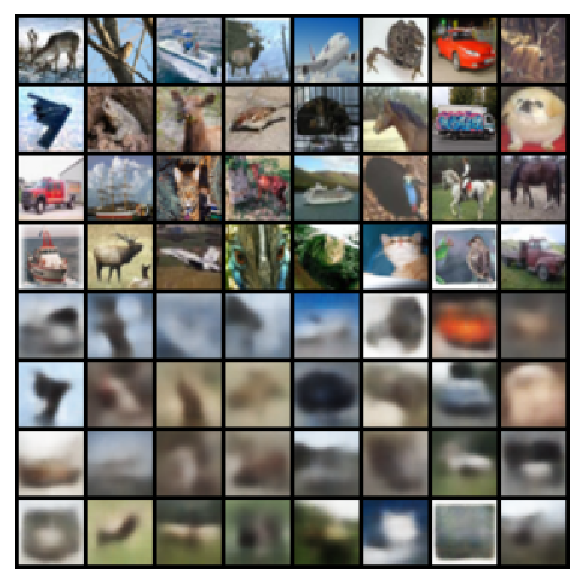
\includegraphics[width=0.45\textwidth]{images/dm/vae_reconstruction}
    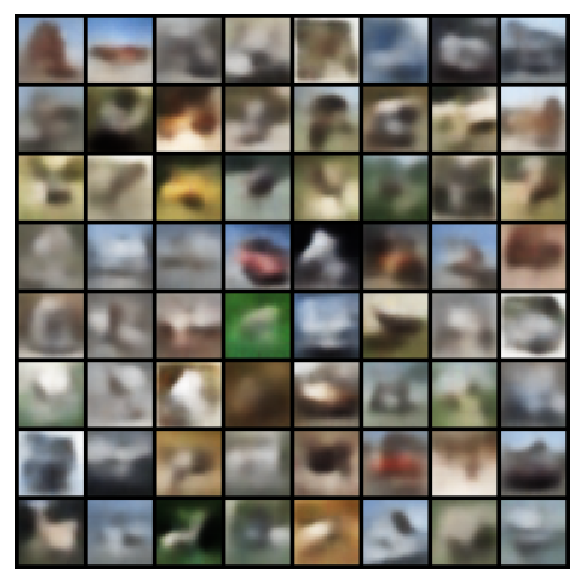
\includegraphics[width=0.45\textwidth]{images/dm/vae_samples}
    \caption{(Izquierda) reconstrucción de imágenes realizada por un VAE sobre el dataset CIFAR-10 utilizando una red convolucional, donde las primeras 4 filas corresponden a las imágenes originales y las últimas 4 filas corresponden a la reconstrucción. (Derecha) generación incondicional de imágenes a partir del VAE. La implementación de este modelo se encuentra en el archivo \texttt{vae.ipynb}.}
    \label{fig:dm/vae_samples}
\end{figure}

\subsubsection{Autoencoders variacionales jerárquicos markovianos}

Una generalización natural de los VAEs consiste en considerar una familia ordenada de variables latentes $z_1,\ldots,z_T$, donde la $t$-ésima variable latente depende de $z_{(t+1):T}$\footnote{La notación $z_{t_1:t_2}$ es una forma compacta de escribir $(z_t)_{t=t_1}^{t_2}$, y será utilizada generalmente para representar modelos jerárquicos.}. Este tipo de modelos se conocen como autoencoders variacionales jerárquicos (HVAE) y corresponden a un paso previo para introducir los modelos de difusión a tiempo discreto en la \autoref{dm/discrete_dm}. La distribución conjunta del decoder de este tipo de modelos se factoriza de la siguiente forma:

\begin{equation}
    \label{eq:joint_hvae_decoder}
    p_\theta(x, z_{1:T})
    = p_\theta(x|z_{1:T})\underbrace{
        \left(\prod_{t=2}^{T} p_\theta(z_{t-1}|z_{t:T})\right)
        p_\theta(z_T)}_{p_\theta(z_{1:T})}.
\end{equation}

Notando que el único cambio en la formulación de un HVAE con respecto al modelo de variable latente simple \eqref{eq:latent_model} fue pasar de $z$ a $z_{1:T}$, se puede obtener directamente una expresión para la ELBO en este nuevo tipo de modelos:

\begin{prop}[ELBO para un HVAE]
    Para el modelo dado en \eqref{eq:joint_hvae_decoder} y considerando una posterior aproximada $q_\phi(z_{1:T}|x)$, la ELBO toma la siguiente forma:

    \begin{equation}
        \label{eq:elbo_mhvae}
        \elbo
        = \E{q_\phi(z_{1:T}|x)}{\log\frac{p_\theta(x,z_{1:T})}{q_\phi(z_{1:T}|x)}}.
    \end{equation}
\end{prop}

Al imponer una condición de independencia markoviana, $p_\theta(z_{t-1}|z_{t:T})=p_\theta(z_{t-1}|z_t)$, se obiene un modelo gráfico $z_T\to z_{T-1}\to\cdots\to z_1\to x$ denominado autoencoder variacional jerárquico markoviano (MHVAE). En este caso, la distribución conjunta del decoder se reduce a

\begin{equation*}
    p_\theta(x, z_{1:T})
    = p_\theta(x|z_1)\left(\prod_{t=2}^{T}
    p_\theta(z_{t-1}|z_t)\right)
    p_\theta(z_T),
\end{equation*}

mientras que el modelo de inferencia aproximada para la posterior $p_\theta(z_{1:T}|x)$ toma la forma

\begin{equation*}
    q_\phi(z_{1:T}|x)
    = q_\phi(z_1|x) \left(\prod_{t=2}^{T} q_\phi(z_t|z_{t-1})\right).
\end{equation*}

En la \autoref{fig:dm/vae_hvae_graph} se puede observar el modelo gráfico asociado a un VAE estándar y un HVAE con un nivel adicional de jerarquía. Si bien esta familia de modelos son interesantes por sí solos, aquí son introducidos únicamente para definir lo que es un modelo de difusión en la siguiente subsección.

\begin{figure}
    \centering
    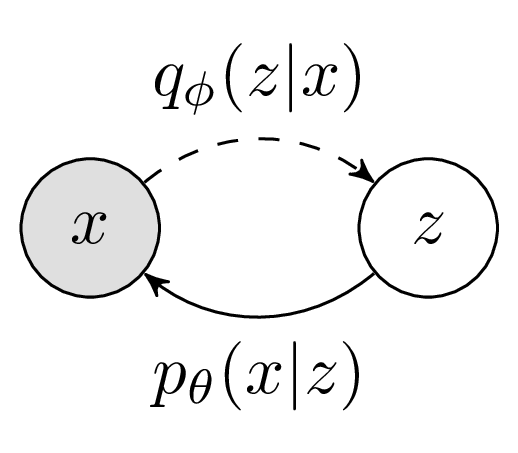
\includegraphics[height=3cm]{images/dm/vae_graph}
    \hspace{1cm}
    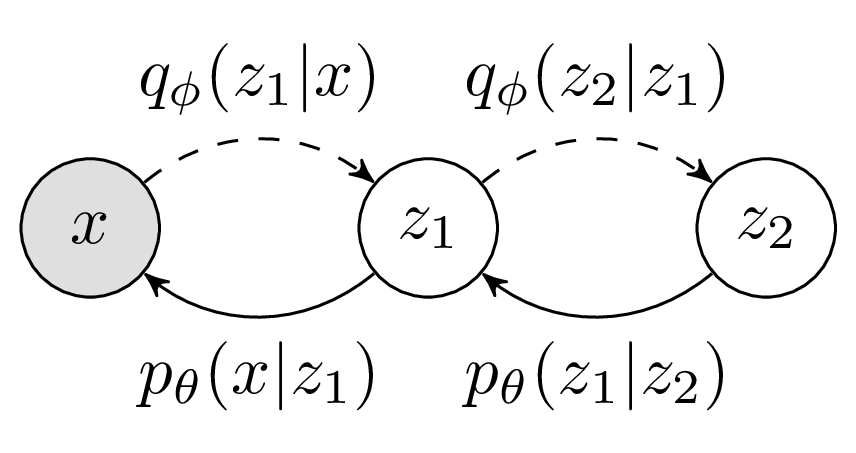
\includegraphics[height=3cm]{images/dm/hvae_graph}
    \caption{Modelo gráfico para un VAE estándar (izquierda) y para un HVAE con dos niveles de jerarquía (derecha). Imágenes obtenidas desde \cite{turner_diffusion_2021}.}
    \label{fig:dm/vae_hvae_graph}
\end{figure}

\section{Modelos de difusión a tiempo discreto}
\label{dm/discrete_dm}

Los modelos de difusión fueron introducidos originalmente el año 2015 en \cite{sohldickstein2015deep}. En esa época, los modelos generativos predominantes eran las GANs (ver \autoref{dm/generative_models/gans}), introducidas un año antes en \cite{goodfellow2014generative}. Debido al gran progreso que se estaba obteniendo en los modelos tipo GAN, el modelo de difusión propuesto en \cite{sohldickstein2015deep} no obtuvo mayor interés hasta el año 2020, cuando investigadores de la universidad de California, en Berkeley, propusieron el modelo \textit{denoising diffusion probabilistic models} (DDPM) en \cite{ho2020denoising}. Los modelos de este tipo actualmente constituyen el estado del arte de los modelos generativos para imágenes, así como en otras modalidades como la generación de audio y video.

De aquí en adelante, a la familia de modelos relacionados con el modelo DDPM se les denominará modelos de difusión.

\subsection{Formulación}
\label{dm/discrete_dm/formulation}

El modelo de difusión propuesto por \cite{ho2020denoising}, puede ser construido como un MHVAE con dos grandes diferencias o imposiciones.

Primero, la dimensión de las variables latentes $z_{1:T}$ es igual a la dimensión de los datos (es decir, $l=d$). Esto contrasta con la noción de cuello de botella vista en el VAE clásico, donde la variable latente $z$, motivada por la \textit{manifold assumption}\footnote{Esta hipótesis afirma que los datos observados realmente provienen de un espacio de menor dimensión (más precisamente, una variedad), el cual está inmerso en el espacio ambiente $\R^d$. Esta suposición permite explicar por qué, aparentemente, las redes neuronales no sufren de la maldición de la dimensionalidad.}, tenía dimensión estrictamente menor a la dimensión observable. Esta nueva restricción permite denotar, con un leve abuso de notación, $(x, z_{1:T})$ como $x_{0:T}$, donde $x_0=x$ y $x_t=z_t$.

La segunda gran diferencia es que ahora el modelo $q_\phi(x_{1:T}|x_0)$ (que originalmente buscaba aproximar la posterior intratable $p_\theta(x_{1:T}|x_0)$) ahora está fijo, por lo que ya no posee parámetros entrenables $\phi$ (por lo que se escribirá únicamente $q$ en vez de $q_\phi$). Más aún, en un modelo de difusión se impone que las transiciones del encoder $q(x_t|x_{t-1})$ sean gaussianas con parámetros (fijos) cuya función será inyectar ruido de tal forma que $q(x_T)\approx\pprior(x_T)$, donde $\pprior$ es una distribución de la cual es fácil generar muestras, por lo que se suele fijar $\pprior(x_T)\sim\gaussian{0}{\identity{d}}$.

Para cumplir estas restricciones, se suele considerar una secuencia finita y decreciente $(\alpha_t)_{t=1}^T\subset[0,1]$ y se definen las siguientes probabilidades de transición de forma autorregresiva para un $x_0\sim\ptrue(x_0)$ dado:

\begin{equation}
    \label{eq:ddpm_forward}
    q(x_{1:T}|x_0) = \prod_{t=1}^{T} q(x_t|x_{t-1}),
    \quad\text{donde}\quad
    q(x_t|x_{t-1}) \sim \gaussian{\sqrt{\alpha_t} x_{t-1}}{(1-\alpha_t)\identity{d}},
    \quad t\in\{1,\ldots,T\}.
\end{equation}

Para un tiempo de difusión $T$ lo suficientemente grande y elecciones de $(\alpha_t)_{t=1}^T\subset[0,1]$ adecuadas (en particular, $\alpha_T\approx 0$), la densidad marginal de $x_T$, $q(x_T)=\int q(x_{0:T})\, dx_{0:(T-1)}$, será aproximadamente $\pprior(x_T)\sim\gaussian{0}{\identity{d}}$. Notar que la igualdad solo se alcanza cuando $T\to\infty$, donde la distribución gaussiana corresponde a la distribución estacionaria del proceso de difusión.

Por otra parte, el decoder $p_\theta(x_{0:T})$ sigue teniendo la misma estructura que antes:

\begin{equation}
    \label{eq:ddpm_backward}
    p_\theta(x_{0:T}) = p_\theta(x_T)\prod_{t=1}^{T} p_\theta(x_{t-1}|x_t),
    \quad\text{donde}\quad
    p_\theta(x_T) = p(x_T) = \pprior(x_T) \sim \gaussian{0}{\identity{d}}.
\end{equation}

Este modelo se interpreta diciendo que el proceso forward $q(x_{1:T}|x_0)$ agrega progresivamente ruido a una muestra $x_0$ generada desde $\ptrue$, mientras que el proceso backward $p_\theta(x_{0:T})$ aprende a deshacer dicha inyección de ruido (\textit{denoising}) comenzando desde $p(x_T)= \pprior(x_T)\approx q(x_T)$. Una ilustración del modelo gráfico asociado al modelo DDPM se puede encontrar en la \autoref{fig:dm/ddpm_model}.

\insertimage{dm/ddpm_model}{1}{Modelo gráfico del proceso de denoising de un DDPM. El proceso comienza con una muestra $x_T\sim p_\text{prior}(x_T)$ y continúa con las transiciones de Markov dadas en \eqref{eq:ddpm_backward} utilizando el modelo $p_\theta$ ya entrenado. La flecha reversa indica el proceso de inyección de ruido realizado durante el entrenamiento. Imagen obtenida desde \cite{ho2020denoising}.}

Por lo tanto, para generar una nueva muestra desde $\ptrue$ teniendo el modelo $p_\theta$ ya entrenado, bastará con generar una muestra $x_T\sim\pprior(x_T)$ y aplicar iterativamente las transiciones de denoising $p_\theta(x_{t-1}|x_t)$ hasta llegar a una muestra $x_0\sim p(x_0)\approx\ptrue(x_0)$.

Antes de pasar a la distribución basal que se utilizará para modelar las transiciones $p_\theta(x_{t-1}|x_t)$ se verán dos propiedades útiles que motivarán su estructura.

\subsubsection{Propiedades de los procesos forward y backward}

El proceso de inyección de ruido definido en \eqref{eq:ddpm_forward} es una cadena de Markov $(x_t)_{t=0}^T$ con distribución inicial $x_0\sim q(x_0)=\ptrue(x_0)$. Por lo tanto, para obtener la muestra ruidosa en tiempo $t$ es necesario conocer la muestra ruidosa en tiempo $t-1$. Si bien esto se puede conseguir iterando mediante $q(x_t|x_{t-1})$, este procedimiento no es eficiente cuando se necesita la distribución en un único tiempo $t\gg 1$. Dado que la cadena tiene transiciones gaussianas, es posible obtener una forma cerrada para $q(x_t|x_0)$:

\begin{prop}[marginal condicional para el proceso forward]
    \label{prop:forward_marginal}
    Bajo las transiciones definidas en \eqref{eq:ddpm_forward}, el proceso forward posee la siguiente propiedad para $t\in\{1,\ldots,T\}$:

    \begin{equation}
        \label{eq:forward_marginal}
        q(x_t|x_0)\sim\gaussian{\sqrt{\overline{\alpha}_t}x_0}{(1-\overline{\alpha}_t)\identity{d}},
        \quad\text{donde}\quad
        \overline{\alpha}_t := \prod\limits_{k=1}^t \alpha_k .
    \end{equation}
\end{prop}

\begin{proof}

    De acuerdo al proceso forward \eqref{eq:ddpm_forward}, $q(x_t|x_{t-1}) \sim \gaussian{\sqrt{\alpha_t} x_{t-1}}{(1-\alpha_t)\identity{d}}$, por lo que una muestra a partir de $(x_t|x_{t-1})$ se puede obtener mediante

    \begin{equation*}
        x_t = \sqrt{\alpha_t} x_{t-1} + \sqrt{1-\alpha_t}\, \epsilon_t,
        \quad
        \epsilon_t\sim\gaussian{0}{\identity{d}}.
    \end{equation*}

    Si $x_{t-1}$ se obtiene del mismo modo a partir de $x_{t-2}$, se llega a que

    \begin{align*}
        x_t &= \sqrt{\alpha_t} \parent{\sqrt{\alpha_{t-1}} x_{t-2} + \sqrt{1-\alpha_{t-1}} \epsilon_{t-1}} + \sqrt{1-\alpha_t}\, \epsilon_t, \quad \epsilon_{t-1},\epsilon_t\sim\gaussian{0}{\identity{d}}\\
        &= \sqrt{\alpha_t\alpha_{t-1}} x_{t-2} + \sqrt{\alpha_t(1-\alpha_{t-1})}\,\epsilon_{t-1} + \sqrt{1-\alpha_t}\,\epsilon_t\\
        &= \sqrt{\alpha_t\alpha_{t-1}} x_{t-2} + \sqrt{[\alpha_t-\alpha_t\alpha_{t-1}]+[1-\alpha_t]}\, \tilde{\epsilon}_{t-1},\quad\tilde{\epsilon}_{t-1}\sim\gaussian{0}{\identity{d}}\\\
        &= \sqrt{\alpha_t\alpha_{t-1}} x_{t-2} + \sqrt{1-\alpha_t\alpha_{t-1}}\, \tilde{\epsilon}_{t-1},
    \end{align*}

    donde en la penúltima igualdad se usó la fórmula de suma de gaussianas. Inductivamente, si todos los $x_t$ se generaron de este modo, se llega a que

    \begin{equation*}
        x_t = \sqrt{\prod_{i=1}^t \alpha_i}\, x_0 + \sqrt{1-\prod_{i=1}^t \alpha_i}\, \tilde{\epsilon}_0,
        \quad\tilde{\epsilon}_0\sim\gaussian{0}{\identity{d}}.
    \end{equation*}

    Es decir,

    \begin{equation*}
        x_t\sim\gaussian{\sqrt{\prod_{i=1}^t \alpha_i}\, x_0}{\parent{1-\prod_{i=1}^t \alpha_i}\identity{d}}.
    \end{equation*}
\end{proof}

Esta propiedad es considerada, generalmente, como una de las más importantes dentro de los modelos de difusión, al punto que se le suele citar, sin hacer referencia explícita, como la \textit{nice property}\footnote{Dado que para el entrenamiento se utiliza esta propiedad, algunos trabajos entregan los niveles de ruidos como secuencias asociadas a la varianza de $q(x_t|x_0)$ y no de $q(x_{t}|x_{t-1})$. Ambos métodos son identificables entre sí.}. Por otra parte, algunas variantes del modelo original de DDPM, como DDIM (ver \autoref{dm/discrete_dm/improvements}) se enfocan en realizar modificaciones al modelo DDPM original buscando preservar precisamente esta propiedad.

Por otra parte, si bien el proceso backward dado en \eqref{eq:ddpm_backward} no es conocido (ya que no se conoce $q(x_0)$), es posible obtener las transiciones inversas cuando se condiciona a $x_0$. Esta propiedad es importante ya que, como se verá más adelante, motivará la forma del proceso reverso $p_\theta(x_{t-1}|x_t)$ en la función de costo de un modelo de difusión aparece una divergencia con esta distribución.

\begin{prop}[proceso inverso condicional a $x_0$]
    \label{prop:conditional_backward}
    Dado el proceso forward definido en \eqref{eq:ddpm_forward}, entonces el proceso inverso dado $x_0$ también es gaussiano y tiene distribución

    \begin{equation}
        \label{eq:conditional_backward}
        q(x_{t-1}|x_t,x_0) \sim \gaussian{\mu_q(x_0,x_t,t)}{\sigma_q^2(t)\identity{d}},
    \end{equation}

    donde la media $\mu_q$ es una combinación lineal entre $x_0$ y $x_t$, mientras que la varianza $\sigma_q^2$ solo depende de $t$. Para $t\geq 2$:

    \begin{equation}
        \label{eq:conditional_backward_params}
        \mu_q(x_0,x_t, t) := \frac{\sqrt{\overline{\alpha}_{t-1}}(1-\alpha_t)}{1-\overline{\alpha}_t}x_0 + \frac{\sqrt{\alpha_t}(1-\overline{\alpha}_{t-1})}{1-\overline{\alpha}_t}x_t
        \quad\text{y}\quad
        \sigma_q^2(t) := \frac{(1-\alpha_t)(1-\overline{\alpha}_{t-1})}{1-\overline{\alpha}_t},
    \end{equation}

    con $\overline{\alpha}_t := \prod\limits_{k=1}^t \alpha_k$. Para $t=1$, se define $\mu_q(x_0,x_t,t)=x_0$ y $\sigma_q^2(t)=0$\footnote{En la práctica, se define como $\sigma_q^2(t)=\epsilon>0$ para que la función de densidad exista y se pueda trabajar con ella posteriormente.}.
\end{prop}

\begin{proof}

    Para $t=1$ es directo ya que $q(x_0|x_1,x_0)\sim\delta_{x_0}$, por lo que se puede considerar como una variable aleatoria gaussiana de media $x_0$ y varianza nula. Para $t>1$, por regla de Bayes y propiedad de Markov:

    \begin{align*}
        q(x_{t-1}|x_t,x_0) & = \frac{q(x_t|x_{t-1})q(x_{t-1}|x_0)}{q(x_t|x_0)}\propto q(x_t|x_{t-1})q(x_{t-1}|x_0)\\
                           & \propto \exp\left[-\frac{1}{2}\left(\frac{\norm{x_t-\sqrt{\alpha_t}x_{t-1}}^2}{1-\alpha_t} + \frac{\norm{x_{t-1}-\sqrt{\overline{\alpha}_{t-1}}x_0}^2}{1-\overline{\alpha}_{t-1}}\right)\right].
    \end{align*}

    Usando las propiedades $\norm{a\pm b}^2=\norm{a}^2\pm 2\langle a,b\rangle + \norm{b}^2$ y $\dotproduct{\lambda a}{b} = \dotproduct{a}{\lambda b}$ para el término dentro del paréntesis y dejando fuera las constantes que no dependen de $x_{t-1}$:

    \begin{align*}
         & \frac{\norm{x_t-\sqrt{\alpha_t}x_{t-1}}^2}{1-\alpha_t} + \frac{\norm{x_{t-1}-\sqrt{\overline{\alpha}_{t-1}}x_0}^2}{1-\overline{\alpha}_{t-1}}\\
         & = \frac{\alpha_t\norm{x_{t-1}}^2-2\dotproduct{\sqrt{\alpha_t}x_{t-1}}{x_t}}{1-\alpha_t} + \frac{\norm{x_{t-1}}^2-2\dotproduct{x_{t-1}}{\sqrt{\overline{\alpha}_{t-1}} x_0}}{1-\overline{\alpha}_{t-1}}+\cte\\
         & =\norm{x_{t-1}}^2\parent{\frac{\alpha_t}{1-\alpha_t}+\frac{1}{1-\overline{\alpha}_{t-1}}}-2\dotproduct{x_{t-1}}{\parent{\frac{\sqrt{\alpha_t}}{1-\alpha_t}x_t + \frac{\sqrt{\overline{\alpha}_{t-1}}}{1-\overline{\alpha}_{t-1}}x_0}} + \cte\\
         & =\frac{1-\overline{\alpha}_{t}}{(1-\alpha_t)(1-\overline{\alpha}_{t-1})}\parent{\norm{x_{t-1}}^2-2\dotproduct{x_{t-1}}{\frac{\sqrt{\alpha_t}(1-\sqrt{\alpha_{t-1}})}{1-\overline{\alpha}_t}x_t+\frac{\sqrt{\alpha_{t-1}}(1-\alpha_t)}{1-\overline{\alpha}_t}x_0}} + \cte .\\
    \end{align*}

    Por lo tanto:

    \begin{equation*}
        q(x_{t-1}|x_t,x_0) \propto \exp\parent{-\frac{1}{2\sigma_q^2(t)}\norm{x_{t-1}-\mu_q(x_0,x_t,t)}^2}.
    \end{equation*}

    La demostración concluye notando que esto define completamente $q(x_{t-1}|x_t,x_0)$ salvo constantes multiplicativas de normalización.
\end{proof}

Una ilustración de las distribuciones encontradas se puede ver en la \autoref{fig:dm/distributions}.

\begin{figure}[!ht]
    \centering
    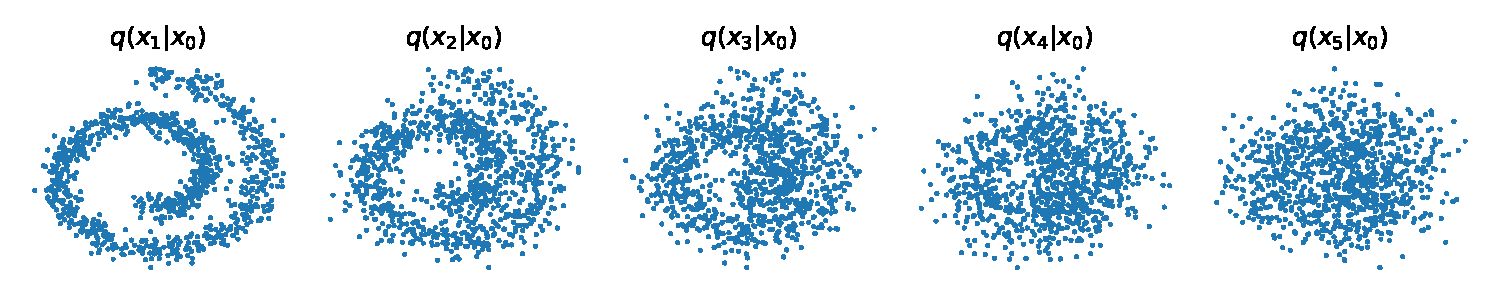
\includegraphics[width=\textwidth]{images/dm/ddpm_forward}
    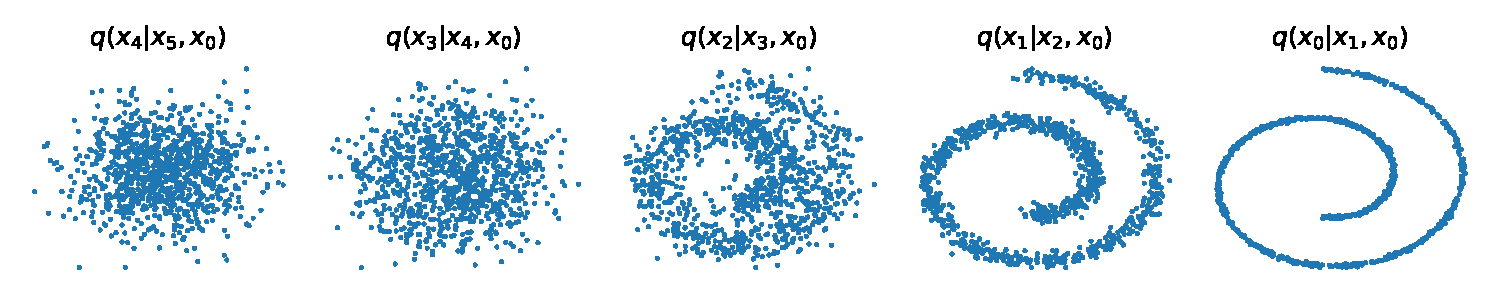
\includegraphics[width=\textwidth]{images/dm/ddpm_conditional_backward}
    \caption{(Arriba) muestras del proceso forward dado por la \autoref{prop:forward_marginal} para $T=5$. (Abajo) muestras del proceso reverso condicional dado por la \autoref{prop:conditional_backward}. La implementación de estas distribuciones se encuentra en el archivo \texttt{ddpm.ipynb}.}
    \label{fig:dm/distributions}
\end{figure}

\subsubsection{Formulación para el proceso inverso}

Motivado por la \autoref{prop:conditional_backward}, se propone elegir un modelo paramétrico gaussiano para el proceso reverso (incondicional) del modelo de difusión:

\begin{equation}
    \label{eq:backward_transition}
    p_\theta(x_{t-1}|x_t)\sim\gaussian{\mu_\theta(x_t,t)}{\Sigma_\theta(x_t,t)},
    \quad t\in\{1,\ldots,T\},
\end{equation}

donde $\mu_\theta$ y $\Sigma_\theta$ son modelos paramétricos entrenados mediante redes neuronales que reciben una muestra ruidosa $x_t$ en un tiempo $t$ y entregan la media y covarianza para la muestra $x_{t-1}$ en el tiempo anterior. Notando que la matriz de covarianza de $q(x_{t-1}|x_t,x_0)$ en \eqref{eq:conditional_backward} es independiente de $x_0$ (solo depende de $t$), los autores de \cite{ho2020denoising} decidieron fijar la varianza de $p_\theta(x_{t-1}|x_t)$ como la varianza de $p_\theta(x_{t-1}|x_t,x_0)$:

\begin{equation}
    \label{eq:backward_covariance}
    \Sigma_\theta(x_t,t):=\Sigma(t):=\sigma_q^2(t)\identity{d},
    \quad t\in\{1,\ldots,T\}.
\end{equation}

Como se verá en el \autoref{teo:elbo_ddpm}, esta elección permitirá simplificar la función objetivo de los modelos de difusión. Los autores también probaron usar $\Sigma(t):=(1-\alpha_{t})\identity{d}$ basándose en la covarianza de $q(x_{t}|x_{t-1})$ según \eqref{eq:ddpm_forward}, que también es independiente de $x_0$. El primer caso corresponde a una cota inferior de la entropía para el proceso reverso, donde $x_0$ concentra toda su masa en un único punto, mientras que el segundo caso corresponde a la cota superior. Ambas elecciones de $\Sigma_\theta(x_t,t)$ entregan resultados similares, necesitando únicamente entrenar una red neuronal para predecir la media $\mu_\theta(x_t,t)\in\R^d$. En el archivo \texttt{ddpm.ipynb} se entrena un modelo de difusión utilizando la varianza dada en \eqref{eq:backward_covariance}.

Es importante notar que nada garantiza, en ninguno de los dos casos, que la covarianza fijada $\Sigma_\theta(x_t,t)$ sea igual a la covarianza realmente buscada, $\var{q(x_{t-1}|x_t)}$, la cual es desconocida\footnote{Ya que no se conoce la distribución $q_0=\ptrue$. Si se conociera, se podría obtener $q(x_{t-1}|x_t)$ usando $q(x_{t-1}|x_t,x_0)$}. En \cite{nichol2021improved} muestran que aprender también la varianza $\Sigma_\theta(x_t,t)$ permite generar muestras en menos pasos sin afectar considerablemente la calidad de las muestras generadas (ver \autoref{dm/discrete_dm/improvements}).

Por otra parte, al igual que los autoencoders variacionales, los modelos de difusión serán entrenados mediante la ELBO. Como se verá a continuación, esta función objetivo puede tomar diferentes formas equivalentes, por lo que, si bien ahora se está entrenando un modelo para predecir la media de $x_{t-1}$ conociendo $x_t$, también se podrá formular el problema para buscar el ruido $\epsilon_t$ insertado a $x_0$ en el tiempo $t$, e incluso se podrá buscar directamente $x_0$.

\subsubsection{ELBO y función objetivo}

Recordando que los modelos de difusión son una MHVAE con condiciones específicas, se puede utilizar la expresión dada en \eqref{eq:elbo_mhvae} para obtener una ELBO conveniente para los modelos de difusión.

\begin{teo}[ELBO para DDPM]
    \label{teo:elbo_ddpm}
    Para un modelo de difusión genérico\footnote{No necesariamente haciendo uso de las transiciones dadas en el lado derecho de \eqref{eq:ddpm_forward}.} factorizado como en \eqref{eq:ddpm_forward} y \eqref{eq:ddpm_backward}, su ELBO viene dada por:

    \begin{equation}
        \label{eq:elbo_ddpm}
        \underbrace{\E{q(x_1|x_0)}{\log p_\theta(x_0|x_1)}}_{\text{término de reconstrucción}} - \underbrace{\KL{q(x_T|x_0)}{p(x_T)}}_{\text{prior matching}} - \sum_{t=2}^T \underbrace{\E{q(x_t|x_0)}{\KL{q(x_{t-1}|x_t,x_0)}{p_\theta(x_{t-1}|x_t)}}}_{\text{denoising matching}}.
    \end{equation}
\end{teo}

\begin{proof}
    Sustituyendo la factorización forward \eqref{eq:ddpm_forward} y la factorización backward \eqref{eq:ddpm_backward} en el ELBO \eqref{eq:elbo_mhvae}:

    \begin{align}
        \elbo &= \E{q(x_{1:T}|x_0)}{\log\parent{\frac{p_\theta(x_{0:T})}{q(x_{1:T}|x_0)}}}\nonumber\\
        &= \E{q(x_{1:T}|x_0)}{\log\parent{\frac{p(x_T)\prod_{t=1}^{T} p_\theta(x_{t-1}|x_t)}{\prod_{t=1}^{T} q(x_t|x_{t-1})}}}\nonumber\\
        &= \E{q(x_{1:T}|x_0)}{\log\parent{p(x_T)\prod_{t=1}^{T}\frac{p_\theta(x_{t-1}|x_t)}{q(x_t|x_{t-1})}}}\label{eq:elbo_ddpm_aux1}.
    \end{align}

    Dado que $q(x_t|x_0)$ y $q(x_{t-1}|x_t,x_0)$ se pueden conocer en forma cerrada, se realiza la siguiente sustitución:

    \begin{equation}
        \label{eq:elbo_ddpm_aux2}
        q(x_t|x_{t-1}) = q(x_t|x_{t-1},x_0) = \frac{q(x_{t-1}|x_t,x_0)q(x_t|x_0)}{q(x_{t-1}|x_0)}.
    \end{equation}

    Sustituyendo \eqref{eq:elbo_ddpm_aux2} en \eqref{eq:elbo_ddpm_aux1} y considerando que $q(x_0|x_0)=1$ y $q(x_0|x_t,x_0)=1$:

    \begin{align*}
        \elbo &= \E{q(x_{1:T}|x_0)}{\log\parent{p(x_T)\prod_{t=1}^{T}\frac{p_\theta(x_{t-1}|x_t)q(x_{t-1}|x_0)}{q(x_{t-1}|x_t,x_0)q(x_t|x_0)}}}\\
        &= \E{q(x_{1:T}|x_0)}{\log p(x_T) + \sum_{t=1}^T \log\parent{\frac{p_\theta(x_{t-1}|x_t)}{q(x_{t-1}|x_t,x_0)}} + \underbrace{\sum_{t=1}^T \parent{\log q(x_{t-1}|x_0)-\log q(x_t|x_0)}}_{\log q(x_0|x_0)-\log q(x_T|x_0)}}\\
        &= \E{q(x_{1:T}|x_0)}{\log\parent{\frac{p(x_T)}{q(x_T|x_0)}} + \log\parent{\frac{p_\theta(x_0|x_1)}{1}} + \sum_{t=2}^T \log\parent{\frac{p_\theta(x_{t-1}|x_t)}{q(x_{t-1}|x_t,x_0)}}}\\
        &= \E{q(x_T|x_0)}{\log \frac{p(x_T)}{q(x_T|x_0)}} + \E{q(x_1|x_0)}{\log p_\theta(x_0|x_1)} + \sum_{t=2}^T \E{q(x_t,x_{t-1}|x_0)}{\log\frac{p_\theta(x_{t-1}|x_t)}{q(x_{t-1}|x_t,x_0)}}\\
        &= -\KL{q(x_T|x_0)}{p(x_T)} + \E{q(x_1|x_0)}{\log p_\theta(x_0|x_1)} - \sum_{t=2}^T \E{q(x_t|x_0)}{\KL{q(x_{t-1}|x_t,x_0)}{p_\theta(x_{t-1}|x_t)}},
    \end{align*}

    donde en la última igualdad se factorizó $q(x_t,x_{t-1}|x_0)=q(x_t|x_0)q(x_{t-1}|x_t,x_0)$ para descomponer la esperanza $\E{q(x_t,x_{t-1}|x_0)}{\cdot}$ como $\E{q(x_t|x_0)}{\E{q(x_{t-1}|x_t,x_0)}{\cdot}}$.
\end{proof}

Notar que el término de reconstrucción es el mismo que aparece en un VAE convencional, por lo que puede ser aproximado mediante estimaciones de Monte Carlo. Sin embargo, como se verá a continuación, no se considerará en la optimización debido a que se trabajará con una función objetivo simplificada. Por otra parte, el término de prior matching puede omitirse en el entrenamiento ya que es constante con respecto a los parámetros del modelo $p_\theta$.

Por último, los términos de denoising matching confirman la elección de las transiciones backward $p_\theta(x_{t-1}|x_t)$ gaussianas, ya que permitirán tener una forma cerrada para este término. Más aún, al elegir $\Sigma_\theta(x_t,t)=\sigma_q^2(t)\identity{d}$ de acuerdo a \eqref{eq:backward_covariance}, la varianza de $q(x_{t-1}|x_t,x_0)$ y $p_\theta(x_{t-1}|x_t)$ coinciden, simplificando aún más la función objetivo. Utilizando el \autoref{teo:kl_gaussians} para este caso particular, se obtiene que:

\begin{align*}
    \KL{q(x_{t-1}|x_t,x_0)}{p_\theta(x_{t-1}|x_t)} & = \frac{1}{2}\left(\frac{\norm{\mu_q(x_0,x_t, t)-\mu_\theta(x_t,t)}^2}{\sigma_q^2(t)}+\trace{\identity{d}}-\log(1)-d\right) \\
                                                   & = \frac{1}{2\sigma_q^2(t)} \norm{\mu_q(x_0,x_t, t)-\mu_\theta(x_t,t)}^2 .
\end{align*}

Por otro lado, para el término de reconstrucción $\E{q(x_1|x_0)}{\log p_\theta(x_0|x_1)}$, es útil recordar de la \autoref{prop:conditional_backward} que, $q(x_{t-1}|x_t,x_0) \sim \gaussian{\mu_q(x_0,x_t,t)}{\sigma_q^2(t)\identity{d}}$. Por lo tanto:

\begin{equation*}
    \log p_\theta(x_0|x_1) = \frac{-1}{2\sigma_q^2(1)}\norm{\mu_q(x_0,x_1,1)-\mu_\theta(x_1,1)}^2 + \cte .
\end{equation*}

En consecuencia, los términos de reconstrucción y denoising matching se pueden agrupar en una única suma (comenzando desde 1), mientras que el término de prior matching se puede omitir dado que es constante con respecto a los parámetros:

\begin{equation*}
    \elbo = \sum_{t=1}^T \frac{1}{2\sigma_q^2(t)} \E{q(x_0,x_t)}{\norm{\mu_q(x_0,x_t, t)-\mu_\theta(x_t,t)}^2} + \cte .
\end{equation*}

Recordando que se busca maximizar la ELBO en esperanza sobre $x_0\sim\ptrue(x_0)$, el problema de optimización asociado a DDPM se reduce a resolver una diferencia de cuadrados:

\begin{prop}[problema de optimización DDPM, $\mu$-prediction]
    \label{prop:mu_prediction}

    Para los modelos propuestos en \eqref{eq:ddpm_forward} y \eqref{eq:backward_transition}, la función de media del proceso reverso, $\mu_\theta(x_t,t)$, que maximixa la ELBO se se encuentra resolviendo el siguiente problema de optimización:

    \begin{equation*}
        \mu_\theta^* = \argmin_{\theta} \sum_{t=1}^T \frac{1}{2\sigma_q^2(t)} \E{q(x_0,x_t)}{\norm{\mu_q(x_0,x_t, t)-\mu_\theta(x_t,t)}^2},
    \end{equation*}

    donde se recuerda que $q(x_0,x_t)=q(x_0)q(x_t|x_0)$ con $q(x_0)\sim\ptrue(x_0)$ y $q(x_t|x_0)$ dado en \eqref{eq:forward_marginal}.
\end{prop}

En la función objetivo anterior, la esperanza $\E{q(x_0,x_t)}{\cdot}=\E{x_0\sim\ptrue}{\E{q(x_t|x_0)}{\cdot}}$ se puede aproximar mediante un conjunto de muestras $(x_0^k)_{k=1}^n\subset\R^d$ para $\E{\ptrue}{\cdot}$ y con un conjunto de muestras ruidosas $(x_t^k)_{k=1}^m$ generadas a partir de cada $x_0^k\sim\ptrue(x_0)$ de acuerdo a $q(x_t|x_0)$.

Si bien la expresión a optimizar es bastante simple de implementar, es posible trabajar un poco más la expresión para disminuirle la carga al modelo paramétrico $\mu_\theta(x_t,t)$. Para esto, se verán dos reformulaciones equivalentes de este problema de optimización.

\paragraph{Enfoque \texorpdfstring{$x_0$}{x0}-prediction}

Notando que $\mu_q(x_0,x_t,t)$ en \eqref{eq:conditional_backward_params} es de la forma $c_1(t)x_0 + c_2(t)x_t$, entonces el modelo $\mu_\theta(x_t,t)$ se puede reparametrizar como $\mu_\theta(x_t,t)=c_1(t)x_\theta(x_t,t) + c_2(t)x_t$, donde ahora $x_\theta$ es otro modelo paramétrico que busca predecir $x_0$ a partir de $x_t$:

\begin{prop}[problema de optimización DDPM, $x_0$-prediction]
    Para los modelos propuestos en \eqref{eq:ddpm_forward} y \eqref{eq:backward_transition}, la función de media del proceso reverso, $\mu_\theta(x_t,t)$, que maximixa la ELBO es una combinación lineal entre $x_\theta$ y $x_t$:

    \begin{equation*}
        \mu_\theta(x_t,t) = \frac{\sqrt{\overline{\alpha}_{t-1}}(1-\alpha_t)}{1-\overline{\alpha}_t}x_\theta(x_t,t) + \frac{\sqrt{\alpha_t}(1-\overline{\alpha}_{t-1})}{1-\overline{\alpha}_t}x_t ,
    \end{equation*}

    donde el modelo $x_\theta(x_t,t)$ resuelve el siguiente problema de optimización:

    \begin{equation*}
        x_\theta^* = \argmin_{x_\theta} \sum_{t=1}^T \frac{\overline{\alpha}_{t-1}(1-\alpha_t)^2}{2\sigma_q^2(t)(1-\overline{\alpha}_t)^2} \E{q(x_0,x_t)}{\norm{x_0-x_\theta(x_t,t)}^2} ,
    \end{equation*}
\end{prop}

\begin{proof}
    Considerando que $\mu_q(x_0,x_t,t)=c_1(t)x_0 + c_2(t)x_t$ y $\mu_\theta(x_t,t)=c_1(t)x_\theta(x_t,t) + c_2(t)x_t$ con $c_1,c_2$ dadas en \eqref{eq:conditional_backward_params}:

    \begin{equation*}
        \norm{\mu_q(x_0,x_t,t)-\mu_\theta(x_t,t)}^2 = \norm{c_2(t)(x_0-x_\theta(x_t,t))}^2 = c_2(t)^2 \norm{(x_0-x_\theta(x_t,t))}^2 ,
    \end{equation*}

    Luego, basta sustituir esta expresión en la \autoref{prop:mu_prediction}.
\end{proof}

\paragraph{Enfoque \texorpdfstring{$\epsilon$}{epsilon}-prediction}

Al igual que para el enfoque $x_0$-prediction, es posible reparametrizar el modelo $\mu_\theta$ usando otro modelo que aprenda el ruido $\epsilon(x_t)$ que se le inyectó a $x_0$ para obtener $x_t$. Para esto es útil notar que, de acuerdo a la \autoref{prop:forward_marginal}, $q(x_t|x_0)\sim \sqrt{\overline{\alpha}_t}x_0 + \sqrt{1-\overline{\alpha}_t}\epsilon$ con $\epsilon\sim\gaussian{0}{\identity{d}}$:

\begin{prop}[problema de optimización DDPM, $\epsilon$-prediction]
    \label{prop:epsilon_prediction}

    Para los modelos propuestos en \eqref{eq:ddpm_forward} y \eqref{eq:backward_transition}, la función de media del proceso reverso, $\mu_\theta(x_t,t)$, que maximixa la ELBO es una combinación lineal entre $x_t$ y $\epsilon_\theta$:

    \begin{equation}
        \label{eq:ddpm_epsilon_prediction}
        \mu_\theta(x_t,t) = \frac{1}{\sqrt{\alpha_t}}x_t - \frac{1-\alpha_t}{\sqrt{\alpha_t(1-\overline{\alpha}_t)}}\epsilon_\theta(x_t,t),
    \end{equation}

    donde el modelo $\epsilon_\theta(x_t,t)$ resuelve el siguiente problema de optimización:

    \begin{equation*}
        \epsilon_\theta^*=\argmin_{\epsilon_\theta} \sum_{t=1}^T \frac{(1-\alpha_t)^2}{2\sigma_q^2(t)(1-\bar\alpha_t)\alpha_t} \E{q(x_0,x_t)}{ \norm{\epsilon(x_t) - \epsilon_\theta(x_t,t)}^2}.
    \end{equation*}

    Donde se ha definido $\epsilon(x_t) = \frac{x_t-\sqrt{\overline{\alpha}_t x_0}}{\sqrt{1-\overline{\alpha}_t}}$.
\end{prop}

\begin{proof}
    Basta probar que $\| \mu_\theta(x_t,t) - \mu_q(x_0,x_t,t) \|^2 = \frac{(1-\alpha_t)^2}{(1-\bar\alpha_t)\alpha_t} \| \epsilon - \epsilon_\theta(x_t,t) \|^2$ para $\mu_\theta$ descrito en el enunciado. Considerando que $x_t = \sqrt{\overline{\alpha}_t}x_0 + \sqrt{1-\overline{\alpha}_t}\epsilon(x_t)$, es posible despejar $x_0$ y obtener $x_0 = \frac{x_t - \sqrt{1-\overline{\alpha}_t}\epsilon(x_t)}{\sqrt{\overline{\alpha}_t}}$. Sustituyendo esta expresión en $\mu_q(x_0,x_t,t)$:

    \begin{align*}
        \mu_q(x_0,x_t,t) & = \frac{\sqrt{\overline{\alpha}_{t-1}}(1-\alpha_t)}{1-\overline{\alpha}_t}\cdot\frac{x_t - \sqrt{1-\overline{\alpha}_t}\epsilon(x_t)}{\sqrt{\overline{\alpha}_t}} + \frac{\sqrt{\alpha_t}(1-\overline{\alpha}_{t-1})}{1-\overline{\alpha}_t}x_t \\
                         & = \left(\frac{\sqrt{\overline{\alpha}_{t-1}}(1-\alpha_t)}{(1-\overline{\alpha}_t)\sqrt{\overline{\alpha}_t}} + \frac{\sqrt{\alpha_t}(1-\overline{\alpha}_{t-1})}{1-\overline{\alpha}_t}\right) x_t
        -\frac{\sqrt{\overline{\alpha}_{t-1}}(1-\alpha_t)\sqrt{1-\overline{\alpha}_t}}{(1-\overline{\alpha}_t)\sqrt{\overline{\alpha}_t}}\epsilon(x_t)                                                                                                                     \\
                         & = \left(\frac{1-\alpha_t}{(1-\overline{\alpha}_t)\sqrt{\alpha_t}} + \frac{\alpha_t - \alpha_t\overline{\alpha}_{t-1}}{(1-\overline{\alpha}_t)\sqrt{\alpha_t}}
        \right)x_t - \frac{(1-\alpha_t)\sqrt{1-\overline{\alpha}_t}}{(1-\overline{\alpha}_t)\sqrt{\alpha_t}}\epsilon(x_t)                                                                                                                                                  \\
                         & =\frac{1-\overline{\alpha}_t}{(1-\overline{\alpha}_t)\sqrt{\alpha_t}}x_t - \frac{1-\alpha_t}{\sqrt{1-\overline{\alpha}_t}\sqrt{\alpha_t}}\epsilon(x_t)                                                                                          \\
                         & =\frac{x_t}{\sqrt{\alpha_t}} - \frac{1-\alpha_t}{\sqrt{(1-\overline{\alpha}_t)\alpha_t}}\epsilon(x_t) ,
    \end{align*}

    donde en la tercera y cuarta igualdad se usó que $\alpha_t\overline{\alpha}_{t-1} = \overline{\alpha}_t$. Dado que $\mu_\theta$ es función de $x_t$, se puede reparametrizar como:

    \begin{equation*}
        \mu_\theta(x_t,t) = \frac{x_t}{\sqrt{\alpha_t}} - \frac{1-\alpha_t}{\sqrt{(1-\overline{\alpha}_t)\alpha_t}}\epsilon_\theta(x_t,t).
    \end{equation*}

    Luego:
    \begin{align*}
        \left\| \mu_\theta(x_t,t) - \mu_q(x_0,x_t,t) \right\|^2 & = \left\| \left(\frac{x_t}{\sqrt{\alpha_t}} - \frac{1-\alpha_t}{\sqrt{(1-\overline{\alpha}_t)\alpha_t}}\epsilon_\theta(x_t,t)\right) - \left(\frac{x_t}{\sqrt{\alpha_t}} - \frac{1-\alpha_t}{\sqrt{(1-\overline{\alpha}_t)\alpha_t}}\epsilon(x_t)\right) \right\|^2 \\
                                                                & = \frac{(1-\alpha_t)^2}{(1-\bar\alpha_t)\alpha_t} \| \epsilon(x_t) - \epsilon_\theta(x_t,t) \|^2 ,
    \end{align*}

    que es lo que se quería probar.
\end{proof}

Si bien este enfoque parece ser el más complicado, en \cite{ho2020denoising} afirman que es el que entregó mejores resultados. Además, en este trabajo los autores consideran una versión simplificada de la función objetivo:

\begin{itemize}
    \item Los ponderadores de las esperanzas son omitidos para que todos los sumandos tengan el mismo peso. En \cite{song2022denoising} justifican esta decisión notando que si los modelos $\epsilon_\theta(x_t,t)$ son independientes en la segunda variable (i.e., se tiene un modelo independiente para cada tiempo), entonces el óptimo global es alcanzado optimizando localmente cada sumando, por lo que la función objetivo se vuelve independiente de los ponderadores.
    \item Con el fin de reducir el costo de entrenamiento, la suma sobre $t\in\{2,\ldots,T\}$ es sustituida por una evaluación aleatoria del tiempo. Para esto consideran una variable discreta uniforme $t\sim\text{Uniform}\left(\{1,\ldots,T\}\right)$ y calculan un único sumando de forma aleatoria en cada iteración del entrenamiento.
\end{itemize}

Con estas modificaciones, la función objetivo que proponen minimizar en \cite{ho2020denoising} con el enfoque $\epsilon$-prediction es la siguiente:

\begin{equation}
    \label{eq:ddpm_simple}
    L_{\text{simple}}(\theta) = \E{x_0\sim\ptrue,t\sim\operatorname{Uniforme}\left(\{1,\ldots,T\}\right),\epsilon\sim\gaussian{0}{\identity{d}}}{\norm{\epsilon-\epsilon_\theta(\sqrt{\overline{\alpha}_t}x_0+\sqrt{1-\overline{\alpha}_t}\epsilon,t)}^2},
\end{equation}

donde se consideró que $q(x_t|x_0)\sim \sqrt{\overline{\alpha}_t}x_0 + \sqrt{1-\overline{\alpha}_t}\epsilon$ con $\epsilon\sim\gaussian{0}{\identity{d}}$ para sustituir $x_t$ en $\epsilon_\theta(x_t,t)$ y cambiar la esperanza $\E{q(x_t|x_0)}{\cdot}$ por $\E{\epsilon\sim\gaussian{0}{\identity{d}}}{\cdot}$.

\subsubsection{Algoritmos de entrenamiento y sampling}

Utilizando el enfoque $\epsilon$-prediction con la función de pérdida simplificada \eqref{eq:ddpm_simple} el algoritmo de entrenamiento consiste en aproximar todas las esperanzas de $L_\text{simple}$ con una estimación de Monte Carlo simple, tal como lo muestra el \autoref{alg:ddpm_training}.

\begin{algorithm}
    \caption{Entrenamiento del modelo DDPM}
    \label{alg:ddpm_training}
    \begin{algorithmic}[1]
        \Require muestras de entrenamiento provenientes de $\ptrue$.
        \Require Modelo $\epsilon_\theta$ (no entrenado) y secuencia $(\alpha_t)_{t=1}^T$.
        \While{no haya convergencia}
        \State Obtener muestra de entrenamiento $x_0\sim\ptrue(x_0)$.
        \State Generar $t\sim\text{Uniform}\left(\{1,\ldots,T\}\right)$.
        \State Generar $\epsilon\sim\gaussian{0}{\identity{d}}$.
        \State Actualizar parámetros de $\epsilon_\theta$ según $\nabla_\theta \norm{\epsilon-\epsilon_\theta(\sqrt{\overline{\alpha}_t}x_0+\sqrt{1-\overline{\alpha}_t}\epsilon,t)}$.
        \EndWhile
    \end{algorithmic}
\end{algorithm}

Por otra parte, como se comentó anteriormente, para la generación de muestras es suficiente generar una muestra desde la distribución prior $p(x_T)=\pprior$ y luego aplicar el proceso backward aprendido. Para esto es necesario recordar que, de acuerdo a la \autoref{prop:epsilon_prediction}, la media $\mu_\theta$ de $p_\theta(x_{t-1}|x_t)$ viene dada por:

\begin{equation*}
    \mu_\theta(x_t,t) = \frac{1}{\sqrt{\alpha_t}}x_t - \frac{1-\alpha_t}{\sqrt{\alpha_t(1-\overline{\alpha}_t)}}\epsilon_\theta(x_t,t),
\end{equation*}

mientras que la matriz de covarianzas para $p_\theta(x_{t-1}|x_t)$ se fijó en \eqref{eq:backward_covariance} como $\Sigma_\theta(x_t,t)=\sigma_q^2(t)\identity{d}$. A este procedimiento de generación se le suele llamar \textit{ancestral sampling} (nombre atribuido en \cite{song2021scorebased}) y se encuentra detallado en el \autoref{alg:ddpm_sampling}. Es importante mencionar que al comenzar el proceso reverso desde la distribución prior se está induciendo un error en la generación, ya que el proceso de difusión en el \autoref{alg:ddpm_training} solo se ejecuta hasta un horizonte de tiempo finito, mientras que la distribución invariante $\gaussian{0}{\identity{d}}$ es alcanzada únicamente cuando $T\to\infty$. Este es un problema intrínseco de los modelos de difusión y puede generar problemas en la generación de muestras tal como se estudia en \cite{debortoli2023diffusion}. En el \autoref{eot_sbp} se entregará una formulación más robusta mediante el problema del puente de Schrödinger, donde se estudiará el problema de transformar una distribución en otra en un horizonte de tiempo finito, permitiendo, además, considerar una distribución terminal $q(x_T)$ diferente a $\gaussian{0}{\identity{d}}$.

\begin{algorithm}
    \caption{Ancestral sampling}
    \label{alg:ddpm_sampling}
    \begin{algorithmic}[1]
        \Require modelo $\epsilon_\theta$ (entrenado) y secuencia $(\alpha_t)_{t=1}^T$ que se usó durante el entrenamiento.
        \State Generar $x_T\sim \pprior(x_T)=\gaussian{0}{\identity{d}}$.
        \For{$t$ desde $T$ hasta 1}
        \If{$t>1$}
        \State generar $z\sim\gaussian{0}{\identity{d}}$
        \Else
        \State $z \gets 0$
        \EndIf
        \State $x_{t-1} \gets \frac{1}{\sqrt{\alpha_t}}\left(x_t-\frac{1-\alpha_t}{\sqrt{1-\overline{\alpha}_t}}\epsilon_\theta(x_t,t)\right) + \sigma_q(t) z$
        \EndFor
        \State \Return $x_0$
    \end{algorithmic}
\end{algorithm}

En la \autoref{fig:dm/ddpm_cifar10} se puede observar la evolución del proceso de denoising en cada etapa del \autoref{alg:ddpm_sampling}, mientras que en la \autoref{fig:dm/ddpm_samples} se observan muestras generadas por un modelo de difusión sobre un dataset bidimensional.

\insertimage{dm/ddpm_cifar10}{0.6}{Proceso de generación de muestras para un modelo entrenado en CIFAR-10. Cada fila es una muestra distinta y cada columna muestra la predicción actual en un tiempo $t$. Imagen obtenida desde \cite{ho2020denoising}.}

\begin{figure}[!ht]
    \centering
    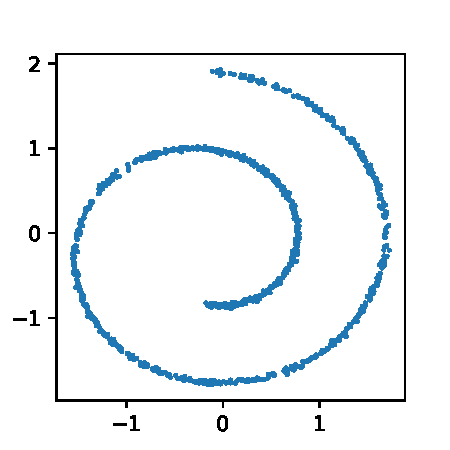
\includegraphics[width=.35\textwidth]{images/dm/ddpm_data}
    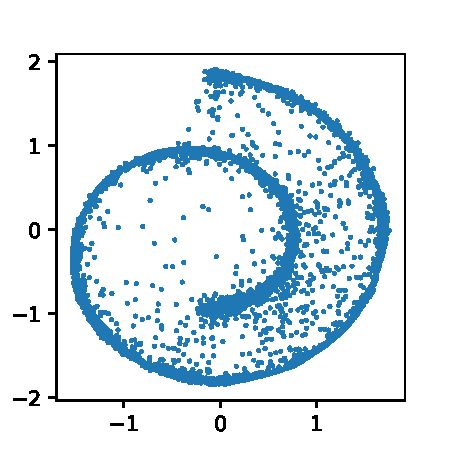
\includegraphics[width=.35\textwidth]{images/dm/ddpm_samples}
    \caption{(Izquierda) batch de entrenamiento para un modelo de difusión. (Derecha) muestras generadas por el modelo de difusión. La implementación de esta técnica se encuentra en el archivo \texttt{ddpm.ipynb}.}
    \label{fig:dm/ddpm_samples}
\end{figure}

\subsection{Arquitectura U-Net para modelos de difusión}
\label{dm/discrete_dm/unet}

Como se ha visto hasta el momento, para aprender $p_\theta(x_{t-1}|x_t)\sim\gaussian{\mu_\theta(x_t,t)}{\Sigma_\theta(x_t,t)}$ se suele entrenar un modelo paramétrico que aprenda directamente $\mu_q$, la muestra original $x_0$ o el ruido $\epsilon$. En cualquiera de estos casos, el modelo es una función de la forma $\R^d\times [0,T]\to\R^d$. Si bien, a priori, es posible utilizar cualquier arquitectura neuronal con estas características, al trabajar con imágenes se suele utilizar una modificación de la arquitectura U-Net \cite{ronneberger2015unet}, cuya arquitectura original se puede observar en la \autoref{fig:dm/u_net_original}.

\insertimage{dm/u_net_original}{0.7}{Arquitectura U-Net original para segmentación de imágenes. Imagen obtenida desde \cite{ronneberger2015unet}.}

En esta subsección se verán las modificaciones usuales que se aplican sobre la arquitectura U-Net para adaptarla a modelos de difusión. En el archivo \texttt{diffusion\_unet.ipynb} se encuentra una implementación detallada de esta arquitectura neuronal junto a las componentes de atención. Es importante destacar que se han propuesto distintas variantes para esta arquitectura, donde el factor común entre ellas son los bloques que las componen. Las principales características son las siguientes:

\begin{itemize}
	\item Se utiliza una red completamente convolucional, donde la parte descendente de la U (ver \autoref{fig:dm/u_net_original}) reduce la resolución a medida que aumenta la cantidad de canales, mientras que la parte ascendente de la U realiza el proceso reverso utilizando convoluciones transpuestas.
	\item En la parte ascendente se realizan conexiones residuales (\textit{skip-connections}) usando los bloques homólogos de la parte descendente.
	\item El tiempo de denoising $t$ es añadido al final de cada bloque convolucional. Para esto se utiliza un embedding temporal sinusoidal similar al usado en la arquitectura \textit{Transformer} \cite{vaswani2023attention}.
	\item Posterior a cada bloque convolucional, luego de sumar el embedding temporal y antes de la conexión residual, se aplica una capa de \textit{multi-head self-attention} similar a la usada en la arquitectura de \textit{Vision Transformer} (ViT) \cite{dosovitskiy2021image}.
	\item Como función de activación se suele usar GELU \cite{hendrycks2023gaussian} y SiLU \cite{elfwing2017sigmoidweighted}, mientras que se suele aplicar normalización por grupos \cite{hafner2018tfdistvae} luego de cada convolución.
\end{itemize}

Una visualización de esta arquitectura modificada puede verse en \autoref{fig:dm/u_net_dm}. En \cite{nichol2021improved} y \cite{dhariwal2021diffusion} se proponen algunas mejoras adicionales sobre esta arquitectura. En particular, los autores de \cite{dhariwal2021diffusion} proponen los siguientes cambios con respecto a la arquitectura usada en el modelo original de DDPM:

\begin{itemize}
	\item Aumentar la profundidad a cambio de ancho, manteniendo una cantidad de parámetros similar.
	\item Aumentar el número de cabezales de atención.
	\item Usar capas de atención en múltiples resoluciones de la U-Net.
	\item Usar los bloques residuales usados en la BigGAN \cite{brock2019largescalegantraining}.
	\item Normalizar las conexiones residuales por $\frac{1}{\sqrt{2}}$.
\end{itemize}

\insertimage{dm/u_net_dm}{1}{Arquitectura U-Net usada para modelos de difusión. El bloque gris representa el input (imagen RGB) mientras que los bloques rosados son bloques convolucionales. Los bloques celestes y verdes son bloques de \textit{downsampling} y \textit{upsampling} respectivamente. Los bloques naranjos son bloques de atención. Por último, las flechas grises son las conexiones residuales. Imagen obtenida desde \cite{erdem2023stepByStepVisualIntroductionToDiffusionModels}.}

Al hacer estos cambios notaron que, si bien el intercambio de ancho por profundidad mejoraba el rendimiento del modelo, también aumentaba el tiempo de entrenamiento necesario para alcanzar el mismo rendimiento en un modelo más ancho. Además, notaron que al aumentar el número de cabezales mejoraba considerablemente el FID\footnote{El FID (\textit{Fréchet inception distance}) es una métrica que mide la similitud entre la distribución real de los datos y la distribución aprendida por un modelo generativo.}. De todos modos, es importante destacar que prácticamente todos los modelos tienen diferentes implementaciones de las arquitecturas U-Net y no existe una arquitectura por defecto (aunque es usual entrenar este modelo usando Adam y \textit{exponential moving average} (EMA) sobre los valores de los parámetros).

Por otra parte, en el último tiempo se ha cambiado el uso de la U-Net por una arquitectura más moderna basada en transformers (\textit{diffusion Transformer} o DiT) \cite{peebles2023scalablediffusionmodelstransformers}, la cual está basada en la arquitectura de \textit{Vision Transformer} (ViT) \cite{dosovitskiy2021image}. En el archivo \texttt{dit.ipynb} hay una implementación minimal de esta arquitectura.

\subsection{Mejoras al modelo DDPM}
\label{dm/discrete_dm/improvements}

En esta subsección se entregarán algunas variantes importantes del modelo propuesto por \cite{ho2020denoising}, las cuales han permitido mejorar aún más la capacidad de los modelos de difusión.

\subsubsection{iDDPM}

En \cite{nichol2021improved}, investigadores de OpenAI realizaron un estudio conocido como \textit{Improved DDPM} donde muestran que aprender la varianza $\Sigma_\theta(x_t,t)$ del proceso backward $p_\theta(x_{t-1}|x_t)$ en \eqref{eq:backward_transition} y utilizar un \textit{variance scheduler} coseno mejora el proceso de inferencia y aumenta la verosimilitud. Además, dan un primer indicio de una \textit{neural scaling law} para DDPM.

\paragraph{Varianza \texorpdfstring{$\Sigma_\theta(x_t,t)$}{} aprendible}

Como se vio anteriormente, el modelo original de DDPM \cite{ho2020denoising} fija la varianza $\Sigma_\theta(x_t,t)$ del modelo reverso $p_\theta(x_{t-1}|x_{t})$ a ser isotrópica: $\Sigma_\theta(x_t,t) = \sigma^2_\theta(x_t,t) \identity{d}$, donde para $\sigma^2_\theta(x_t,t)$ se prueban dos opciones, ambas independientes de $x_t$:

\begin{itemize}
    \item $\sigma^2_\theta(x_t,t) = \sigma_q^2(t)$ de acuerdo a la varianza del proceso reverso condicional a $x_0$, $q(x_{t-1}|x_t,x_0)$ (ver \eqref{eq:backward_covariance}). Fijar esta covarianza permite simplificar la divergencia $\KL{q(x_{t-1}|x_t,x_0)}{p_\theta(x_{t-1}|x_t)}$ en la función de costo \eqref{eq:elbo_ddpm}, llegando a un problema de mínimos cuadrados entre las medias de ambas distribuciones.
    \item $\sigma^2_\theta(x_t,t) = 1-\alpha_t$ de acuerdo a la varianza del proceso forward $q(x_t|x_{t-1})$ (ver \eqref{eq:ddpm_forward}).
\end{itemize}

Dado que ninguna de las dos varianzas es la verdadera, en \cite{nichol2021improved} deciden modelar $\sigma^2_\theta(x_t,t)$ como una interpolación de estos dos valores en el espacio logarítmico:

\begin{equation*}
    \sigma^2_\theta(x_t,t):= \exp\parent{v_\theta(x_t,t)\log (1-\alpha_t) + (1-v_\theta(x_t,t))\log \sigma^2_q(t)},
\end{equation*}

donde $v_\theta(x_t,t)$ es un modelo neuronal. A priori, la varianza aprendida $\sigma^2_\theta(x_t,t)$ podría estar fuera del intervalo formado por $\sigma_q^2(t)$ y $1-\alpha_t$, pero eso no ocurre en la práctica, mostrando que interpolar entre estos valores es una buena parametrización.

\paragraph{Sampling con menos iteraciones}

Dado que el proceso forward por lo general tiene muchas iteraciones ($T=1000$ en DDPM), el proceso reverso tendrá la misma cantidad de iteraciones, haciendo que la generación sea un proceso lento. En \cite{nichol2021improved} descubrieron de forma inesperada que al permitir entrenar la varianza $\Sigma_\theta(x_t,t)$ es posible obtener muestras a partir de un modelo ya entrenado usando menos pasos de los que se usaron durante el entrenamiento y sin la necesidad de hacer \textit{fine-tuning}. Las muestras que se generan de esta forma siguen siendo de alta calidad y permite generar imágenes en segundos en vez de minutos.

Para disminuir la cantidad de iteraciones durante la generación, consideraron una sub-secuencia decreciente de tiempos $S=(S_t)_{t=1}^{|S|}\subset\{0,\ldots,T\}$ con $\{0,T\}\in S$. Dado que $v_\theta(x_{S_t},S_t)$ es el parámetro que define $\sigma_\theta(x_{S_t},S_t)$ mediante interpolación de las varianzas $1-\alpha_{S_t}$ y $\sigma_q^2$, este parámetro será invariante al reescalar los rangos en procesos de difusión más cortos, por lo que se puede hacer el proceso reverso utilizando únicamente los tiempos de $S$ y generando desde $p_\theta(x_{S_{t-1}}|x_{S_t})$ mediante $\gaussian{\mu_\theta(x_{S_t}, S_t)}{\Sigma_\theta(x_{S_t}, S_t)}$.

Con esta técnica, se puede mantener la calidad de generación incluso tomando subconjuntos $S$ de largo 100. Al intentar hacer esto mismo en el modelo original de DDPM hay una pérdida considerable de calidad al disminuir el número de iteraciones.

\paragraph{Función objetivo híbrida}

La función objetivo $L_{\text{simple}}$ (ver \eqref{eq:ddpm_simple}) usada en DDPM solo es válida cuando se fija $\Sigma_\theta(x_t,t) = \sigma_q^2(t)\identity{d}$. Para un modelo que aprende la varianza, se deben volver a computar las expresiones para las divergencias en la ELBO (ver \eqref{eq:elbo_ddpm}). Sin embargo, en \cite{nichol2021improved} obtienen dificultades para optimizar esta nueva función objetivo y observan que la media del proceso reverso, $\mu_\theta$, es más importante que la varianza $\Sigma_\theta$. Por lo tanto, proponen mantener la función simplificada $L_{\text{simple}}$ (que estima bien la media) y combinarla cónicamente con (el negativo de) la ELBO real:

\begin{equation*}
    L_{\text{híbrido}} := L_{\text{simple}} - \lambda\cdot\elbo ,
\end{equation*}

donde $\lambda>0$ es un ponderador y la $\elbo$ de un DM está dada en \eqref{eq:elbo_ddpm}.

Por otra parte, si bien es esperable alcanzar mayores verosimilitudes optimizando directamente la ELBO, los autores observan que se obtienen mejores resultados optimizando esta función objetivo híbrida.

\paragraph{Cosine scheduler}

Otra observación importante es que al usar un \textit{variance scheduler} lineal como en \cite{ho2020denoising} la difusión ocurre muy rápido, destruyendo una gran cantidad de información al comienzo del proceso. En la \autoref{fig:dm/linear_cosine_scheduler} (arriba) se puede observar este fenómeno. Para corregir este problema, proponen un scheduler para $(\bar\alpha_t)_{t=1}^T$\footnote{Esto ya que al entrenar usando \eqref{prop:forward_marginal}, $\alpha_t$ es un parámetro más natural para definir que $\alpha_t$. Sin embargo, ambas formas son equivalentes ya que $\alpha_t=\frac{\bar\alpha_t}{\bar\alpha_{t-1}}$.} que inyecte el ruido más lento:

\begin{equation*}
    \bar\alpha_t = \frac{f(t)}{f(0)},\qquad f(t)=\cos^2\parent{\frac{\frac{t}{T}+s}{1+s}\cdot\frac{\pi}{2}} ,
\end{equation*}

\insertimage{dm/linear_cosine_scheduler}{1}{(arriba) Proceso de difusión asociado a un scheduler lineal. (abajo) Proceso de difusión asociado a un scheduler coseno. Imagen obtenida desde \cite{nichol2021improved}.}

donde $s>0$ (de \textit{smoothing}) es un parámetro de suavizado que permite que la inyección de ruido ocurra de forma más suave al comienzo. Este funcional de ruido tiene un comportamiento lineal en el centro, mientras que en los extremos del intervalo $[0,T]$ el decaimiento es más suave. Es importante notar que el nivel de corrupción visual obtenido en una muestra de $q(x_t|x_0)$ (para un cierto nivel de ruido $1-\bar\alpha_t$) depende de la resolución de la imagen, por lo que este scheduler puede dejar de ser útil en otras resoluciones. En \cite{chen2023importancenoiseschedulingdiffusion} estudian más en detalle el efecto del \textit{scheduler} en el proceso de difusión.

\paragraph{Neural scaling law para los modelos de difusión}

En los últimos años se ha visto que algunos modelos basados en redes neuronales siguen un patrón claro al comparar el rendimiento del modelo con el número de parámetros y la cantidad de datos. Por ejemplo, en \cite{kaplan2020scaling} estudian cómo cambia la entropía cruzada en un \textit{large language model} (LLM) cuando se utiliza una arquitectura tipo \textit{transformer} y encuentran relaciones en forma de potencia entre esta y el número de parámetros, el tamaño del dataset y la capacidad de cómputo del entrenamiento. En \cite{farhani2022momentum} generalizan este resultado al estudiar el transformer como modelo autorregresivo en otras modalidades como imagen o video.

Para modelos de difusión, en \cite{nichol2021improved} notaron que, usando la función objetivo $L_{\text{híbrido}}$, el modelo DDPM mejora de forma predecible al aumentar el cómputo de entrenamiento. Más específicamente, observan que el FID escala siguiendo una ley de potencia, igual que para la entropía cruzada en un LLM. Para la log-verosimilitud, no se observó un patrón claro, sugiriendo que el aumento de cómputo durante el entrenamiento no favorece tan notoriamente al aumento de la verosimilitud. Es importante mencionar que tener una ley que prediga el rendimiento de una familia de modelos generativos es una propiedad sumamente valiosa, lo que puede verse como otra motivación para usar las buenas técnicas empleadas en los modelos de difusión en enfoques más generales como el problema puente de Schrödinger estudiado en el \autoref{eot_sbp}.

\subsubsection{Procesos de difusión no markovianos}

Como se mencionó anteriormente, una de las principales desventajas de los modelos de difusión es su velocidad para generar muestras. Dado que el proceso de denoising está compuesto por varias etapas, la generación de muestras es mucho más lenta que la generación con GANs.

En un trabajo paralelo a iDDPM, los autores de \cite{song2022denoising} notaron que durante el cálculo de la función de pérdida del modelo DDPM, el proceso (markoviano) forward solo es usado a través de las marginales condicionales $q(x_t|x_0),\,t\in\{1\ldots,T\}$ y no a través de la distribución conjunta $q(x_{1:T}|x_0)$ (ver \autoref{alg:ddpm_training}). Con esta observación, en \cite{song2022denoising} definieron una nueva familia de procesos forward, $\mathcal{Q} = \left\{q_\sigma(x_{1:T}|x_0)\right\}_{\sigma\in\mathbb{R}_+^T}$, tales que sus marginales condicionales $q_\sigma(x_t|x_0)$ coincidieran con las del modelo DDPM, es decir, tales que

\begin{equation*}
    q_\sigma(x_t|x_0) = \mathcal{N}\left(\sqrt{\overline{\alpha}_t}x_0,(1-\overline{\alpha}_t)I_d\right).
\end{equation*}

Los procesos forward de la familia $\mathcal{Q}$ son dados de forma implícita mediante la imposición de la forma que deben tener sus procesos reversos:

\begin{equation*}
    q_\sigma(x_{t-1}|x_t,x_0)\sim\mathcal{N}\left(f_{\sigma_t}(x_0,x_t),\sigma_t^2 I_d\right),
\end{equation*}

donde $f_{\sigma_t}:\mathbb{R}^d\times\mathbb{R}^d\to\mathbb{R}^d$ es una función con una forma precisa (conocida) para que se logre la igualdad de las marginales condicionales $q_\sigma(x_t|x_0)$ que se mencionó más arriba. Notar que no es necesario conocer estos procesos forward ya el enfoque DDIM se utiliza cuando el modelo ya está entrenado.

En este trabajo argumentan que, dado que el nuevo proceso forward es indistinguible del proceso forward de DDPM durante el cálculo de la función de pérdida (ya que $q_\sigma(x_t|x_0)$ y $q(x_t|x_0)$ coinciden), entonces el modelo entrenado sirve tanto para el denoising de DDPM como para el denoising de este nuevo proceso de difusión (más específicamente, ellos muestran una equivalencia en el problema de optimización bajo ciertas hipótesis razonables). Por lo tanto, se puede usar la red neuronal ya entrenada en DDPM como si hubiese sido entrenada para este nuevo proceso.

De esta forma, considerando que la red neuronal $\epsilon_\theta(x_t,t)$ busca predecir el ruido $\epsilon$ inyectado a $x_0$ en la etapa $t$, el proceso de generación de muestras que ellos proponen se puede ver en el \autoref{alg:ddim_sampling}.

\begin{algorithm}
    \caption{Generación usando DDIM}
   \label{alg:ddim_sampling}
   \begin{algorithmic}[1]
   \Require modelo $\epsilon_\theta$ (entrenado), secuencia $(\alpha_t)_{t=1}^T$, subsecuencia temporal $\tau = (\tau_1, ..., \tau_S)$ donde $\tau_S = T$.
   \State Generar $x_T \sim q_{\text{prior}}(x_T)$
   \For{$t$ desde $S$ hasta 1}
   \State Estimar $x_0$: $\hat{x}_0 \gets \frac{x_{\tau_t} - \sqrt{1-\overline{\alpha}_{\tau_t}}\epsilon_\theta(x_{\tau_t},\tau_t)}{\sqrt{\overline{\alpha}_{\tau_t}}}$
   \If{$t > 1$}
   \State $x_{\tau_{t-1}} \gets \sqrt{\overline{\alpha}_{\tau_{t-1}}}\hat{x}_0 + \sqrt{1-\overline{\alpha}_{\tau_{t-1}}-\sigma_t^2}\cdot\frac{x_{\tau_t}-\sqrt{\overline{\alpha}_{\tau_t}}\hat{x}_0}{\sqrt{1-\overline{\alpha}_{\tau_t}}}$
   \EndIf
   \EndFor
   \State \Return $x_0 \gets \hat{x}_0$
   \end{algorithmic}
\end{algorithm}

La formulación de $q_\sigma(x_{t-1}|x_t,x_0)$ permite definir diferentes procesos de denoising (y respectivos procesos forward). Más aún, eligiendo un cierto parámetro de proceso $\sigma\in\mathbb{R}^d_+$ es posible hacer el proceso markoviano y recuperar la formulación original de DDPM. Sin embargo, el modelo de interés se consigue en el caso límite cuando $\sigma_t\to 0,\,\forall t\in\{1,\ldots, T\}$ ya que de este modo, el proceso reverso se vuelve determinista. Este es el modelo que en el paper denominan DDIM. Este determinismo permite, al menos en teoría, obtener directamente $x_0$ a partir de $x_T$. Si bien esto no funciona bien en la práctica debido a la alta complejidad del proceso de difusión, es posible realizar el proceso reverso en menos pasos bajo la justificación de que $x_T$ define totalmente $x_0$ desde un comienzo.

Por otra parte, este determinismo está íntimamente relacionado con la \textit{probability flow ODE} de los modelos de difusión en tiempo continuo (ver \autoref{dm/continuous_dm/sde_dm}), la cual a su vez es usada para mostrar que los modelos de difusión aprenden (o al menos aproximan) un mapa de transporte óptimo entre la distribución de los datos y la distribución prior, lo cual es estudiado en la \autoref{ot/dynamic/dm}. En consecuencia, esta es una primera conexión directa con el problema estático del puente de Schrödinger estudiado en la \autoref{eot_sbp/static_sbp}.

\subsubsection{Generación condicional}

Es posible modificar el modelo de difusión estudiado hasta ahora para que funcione como un modelo generativo condicional. Una primera opción para hacer esto es entrenar un modelo de difusión que aprenda una distribución condicional $\ptrue(x|y)$, donde $y$ es una entrada adicional al modelo que indica información acerca de la muestra $x$ que se está generando. Por ejemplo, $y$ podría ser una clase o una descripción de texto de $x$, la cual se puede inyectar al modelo utilizando un embedding vectorial de $y$ concatenado al embedding temporal de $t$. En el caso que $y$ sea un prompt de texto, el embedding se puede obtener mediante un modelo tipo BERT (ver \cite{devlin2019bertpretrainingdeepbidirectional}) o tipo CLIP (ver \cite{radford2021learningtransferablevisualmodels}).

Si bien esta es una técnica usual que se puede emplear en otros modelos como GANs (\autoref{dm/generative_models/gans}) y VAEs (\autoref{dm/vae}), en esta sección se revisará una técnica de condicionamiento llamada \textit{guidance} que es específica para los modelos de difusión (o más generalmente, para los modelos basados en score).

\paragraph{Classifier-guidance}

Para introducir la técnica de \textit{guidance}, se usará un resultado posterior que afirma que los modelos de difusión (que buscan aprender la función de media $\mu_q(x_t,x_0,t)$) se pueden reparametrizar por otro modelo $s_\theta(x_t,t)$ que aprenda la función de score $\score{x_t}{q(x_t)}$. En efecto, de acuerdo a la \autoref{prop:score_prediction} se puede reparametrizar el modelo como

\begin{equation*}
    \label{eq:score_mean_relationship}
    \mu_\theta(x_t,t) = \frac{1}{\sqrt{\alpha_t}}x_t - \frac{1-\alpha_t}{\sqrt{\alpha_t}}s_\theta(x_t,t).
\end{equation*}

Esta propiedad permite trabajar directamente con la función de score de un modelo de difusión condicional, el cual busca aprender, para cada tiempo $t\in\{1,\ldots,T\}$, una función de score $\score{x_t}{p_\theta(x_t|y)}$ para luego poder generar muestras desde $\ptrue(x|y)$. Para conseguir esto es importante notar lo siguiente:

\begin{align}
    p_\theta(x_t|y) = \frac{p_\theta(y|x_t)p_\theta(x_t)}{p_\theta(y)} &\implies \log p_\theta(x_t|y) = \log p_\theta(y|x_t) + \log p_\theta(x_t) - \log p_\theta(y)\nonumber\\
    &\implies \score{x_t}{p_\theta(x_t|y)} = \score{x_t}{p_\theta(y|x_t)} + \score{x_t}{p_\theta(x_t)}\label{eq:classifier_guidance} .
\end{align}

En consecuencia, si $\score{x_t}{p_\theta(x_t)}$ es un modelo de difusión incondicional ya entrenado (el cual se obtiene mediante \eqref{eq:score_mean_relationship}), bastaría con tener un modelo discriminativo $p_\theta(y|x_t)$ para poder generar muestras desde $\ptrue(x|y)$ a partir del modelo de difusión incondicional. Notar que la distribución $p_\theta(y|x_t)$ corresponde a la de un clasificador que es entrenado sobre pares $(x_t,y)$ para cada tiempo $t\in\{1,\ldots,T\}$, lo que motiva el nombre \textit{classifier-guidance} para esta técnica. Notar que la condición $y$ no necesariamente debe tener naturaleza categórica, si no que puede ser un texto, donde $p(y|x)$ suele ser calculado por un modelo tipo CLIP \cite{radford2021learningtransferablevisualmodels}.

Por otra parte, notar que la cantidad $\score{x_t}{p_\theta(y|x_t)}$ no es una función de score ya que el gradiente es tomado con respecto a $x_t$ y no $y$. Sin embargo, $p(y|x_t)$ sí es una densidad de probabilidad, por lo que se puede aplicar la idea de temperatura usada en los modelos de lenguaje\footnote{\interlinepenalty = 10000 Esta técnica consiste en aumentar ($\gamma>1$) o aminorar ($0<\gamma<1$) la concentración de la masa en las modas de una distribución de probabilidad elevando la función densidad a una potencia $\gamma$. En rigor, el parámetro de temperatura es $\frac{1}{\gamma}$, por lo que $\gamma$ se conoce como temperatura inversa.}, donde $p_\theta(y|x_t)$ es cambiada por una densidad proporcional a $p(y|x_t)^\gamma$ con $\gamma>0$. Con este cambio, se puede obtener el score para una nueva distribución $\tilde{p}_\theta(x_t|y)$ (dependiente de $\gamma$), diferente a la distribución $p_\theta(x_t|y)$ en \eqref{eq:classifier_guidance}:

\begin{equation}
    \label{eq:guidance_temperature}
    \tilde{p}_\theta(x_t|y) \propto p_\theta(y|x_t)^\gamma p_\theta(x_t)
    \implies
    \score{x_t}{\tilde{p}_\theta(x_t|y)} = \gamma\,\score{x_t}{p_\theta(y|x_t)} + \score{x_t}{p_\theta(x_t)}.
\end{equation}

Es decir, utilizando este nuevo score condicional es posible generar muestras de la distribución $\ptrue(x|y)$, pero asignándole un peso relativo a la señal $y$ mediante el ponderador $\gamma$. En la \autoref{fig:dm/guidance} se puede observar el efecto de aumentar el \textit{guidance scale} $\gamma$.

\begin{figure}[!ht]
    \centering
    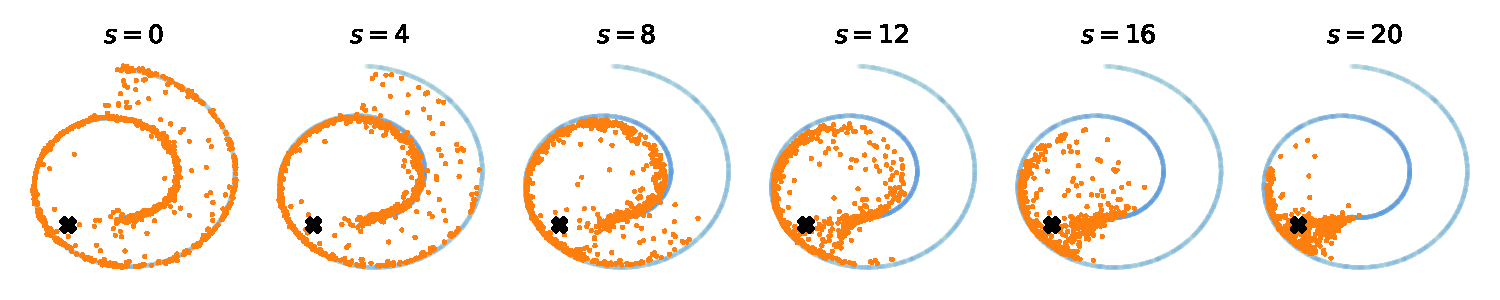
\includegraphics[width=\textwidth]{images/dm/guidance[-1, -1]}
    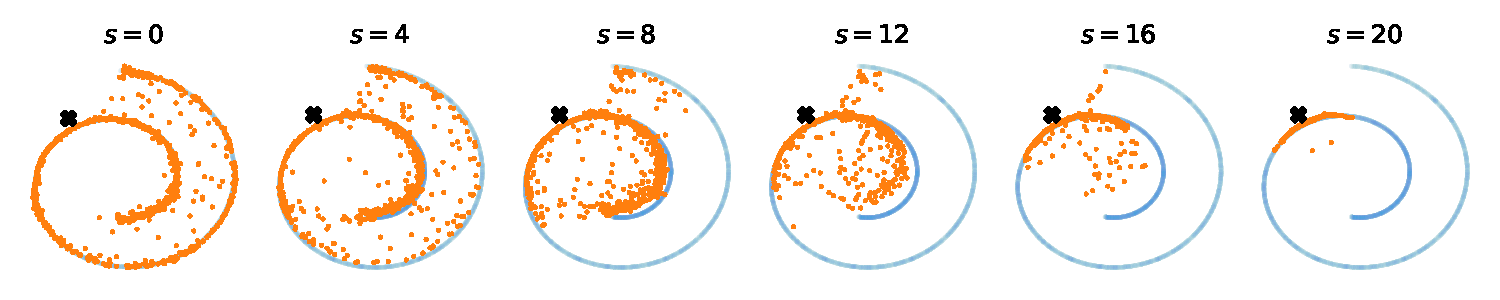
\includegraphics[width=\textwidth]{images/dm/guidance[-1, 1]}
    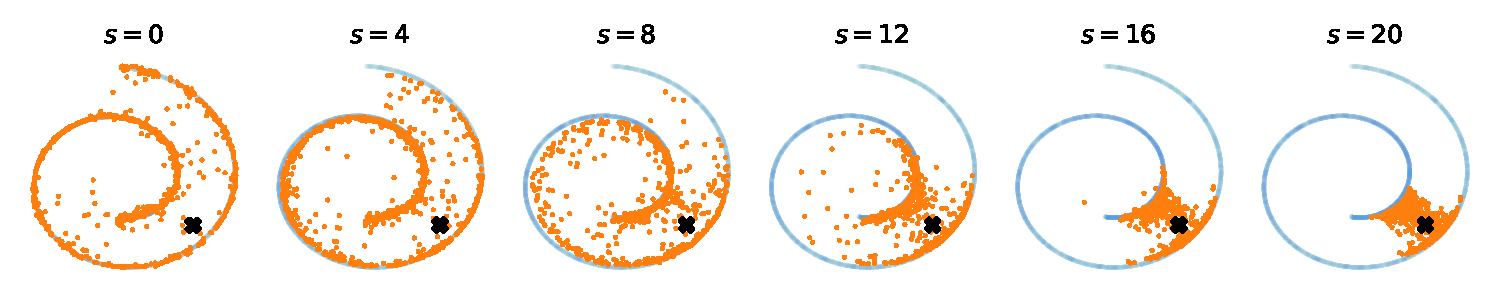
\includegraphics[width=\textwidth]{images/dm/guidance[1, -1]}
    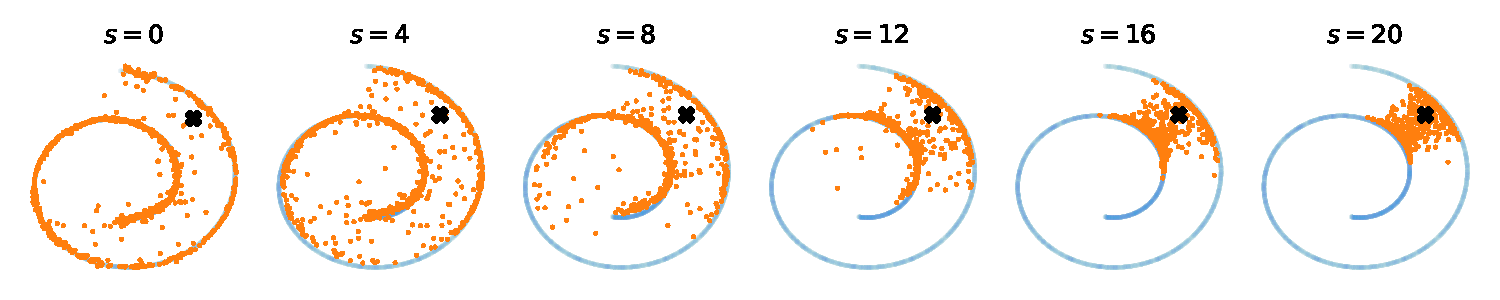
\includegraphics[width=\textwidth]{images/dm/guidance[1, 1]}
    \caption{Desviación de la distribución aprendida por el modelo incondicional $p_\theta(x)$ según la escala de \textit{guidance} (aquí denotado por $s$). El modelo discriminativo $p_\theta(y|x)$ le da un alto valor a puntos cercanos a la cruz marcada en negro. La implementación de esta técnica se encuentra en el archivo \texttt{ddpm.ipynb}.}
    \label{fig:dm/guidance}
\end{figure}

Notar que este factor, al igual como ocurre en el modelamiento del lenguaje, implica un trade-off entre calidad y diversidad ya que al aumentar el parámetro $\gamma$, se están concentrando aún más las modas del modelo discriminativo $p_\theta(y|x_t)$. Esto se puede observar en la \autoref{fig:dm/classifier_guidance_scale} y en la \autoref{fig:glide}.

\insertimage{dm/classifier_guidance_scale}{1}{Trade-off entre calidad y variedad que se observa al cambiar el factor de escala del gradiente. Por un lado, al aumentar el factor aumenta el FID, IS y la precisión (indicadores asociados a la calidad), mientras que disminuye el recall (indicador asociado a la diversidad). Imagen obtenida desde \cite{nichol2022glidephotorealisticimagegeneration}.}

\begin{figure}
    \centering
    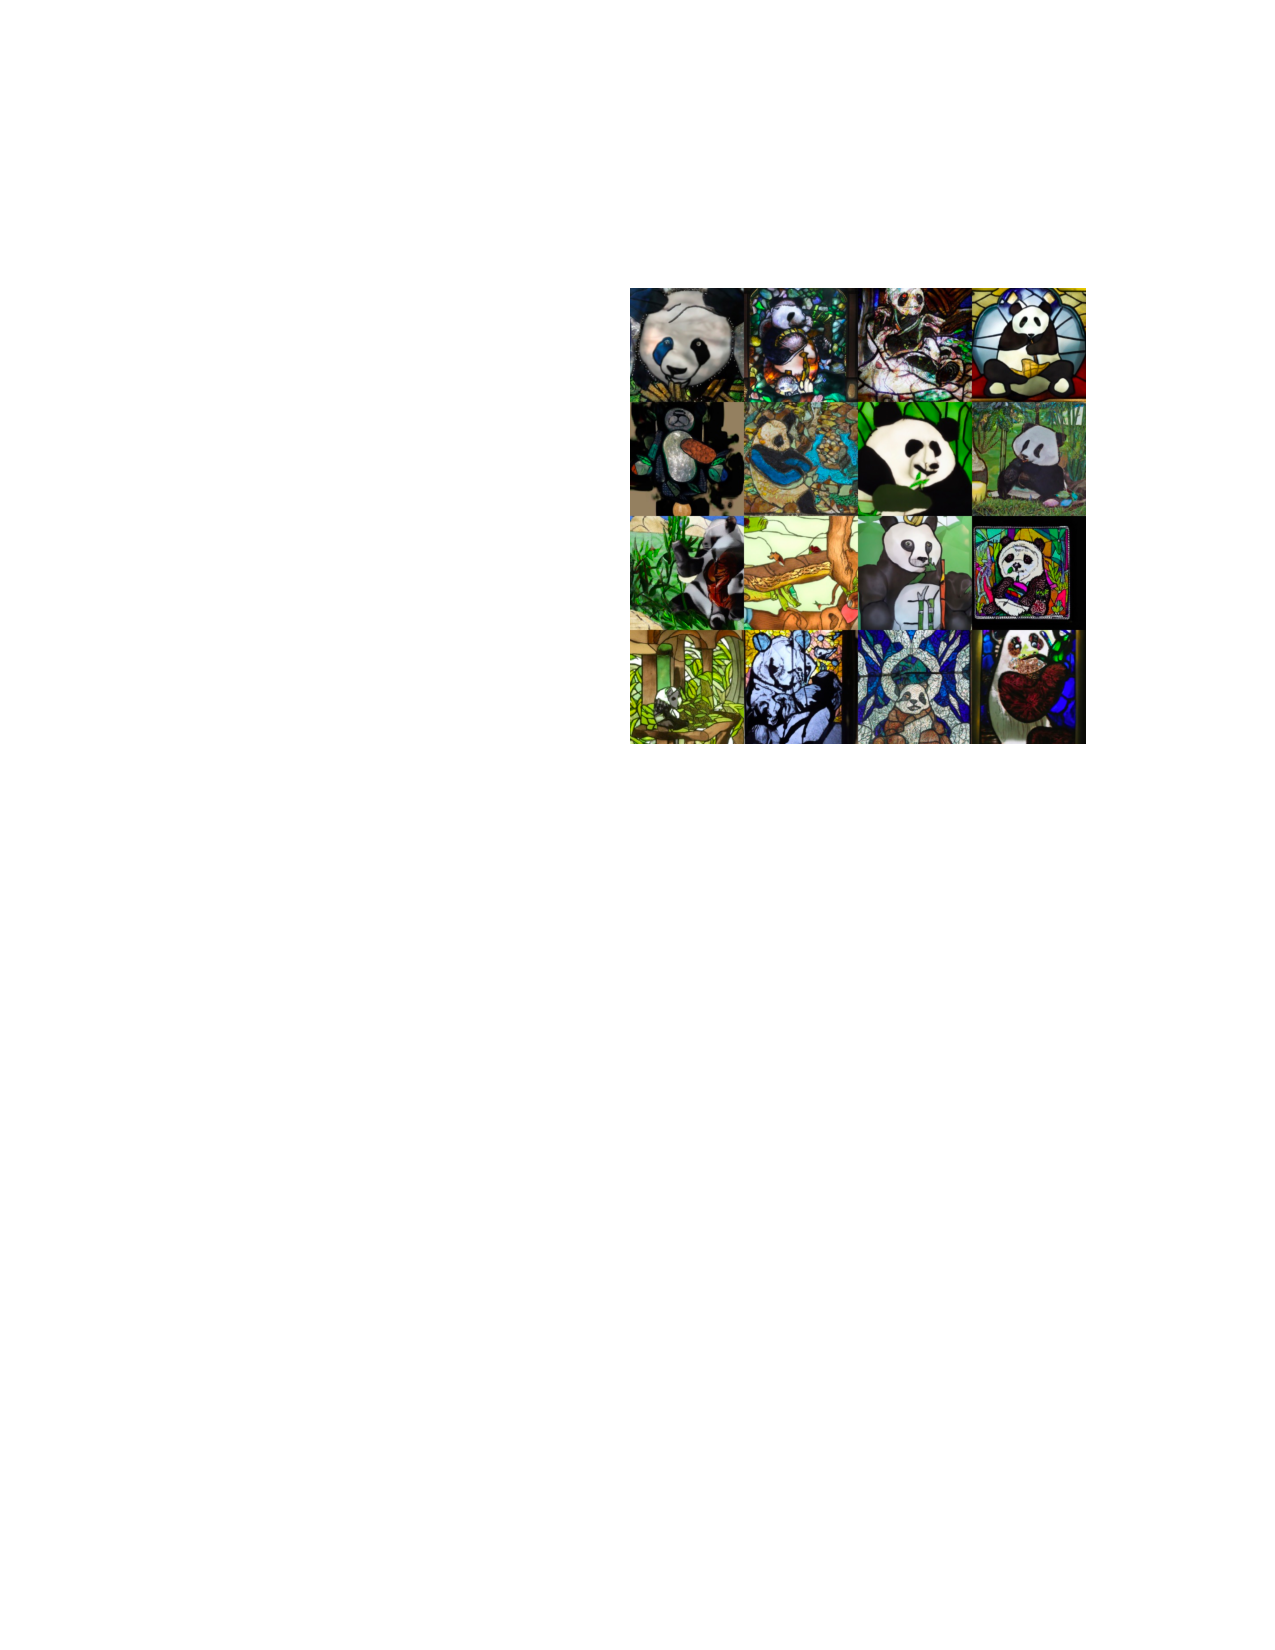
\includegraphics[width=0.45\textwidth]{images/dm/glide_unconditional}
    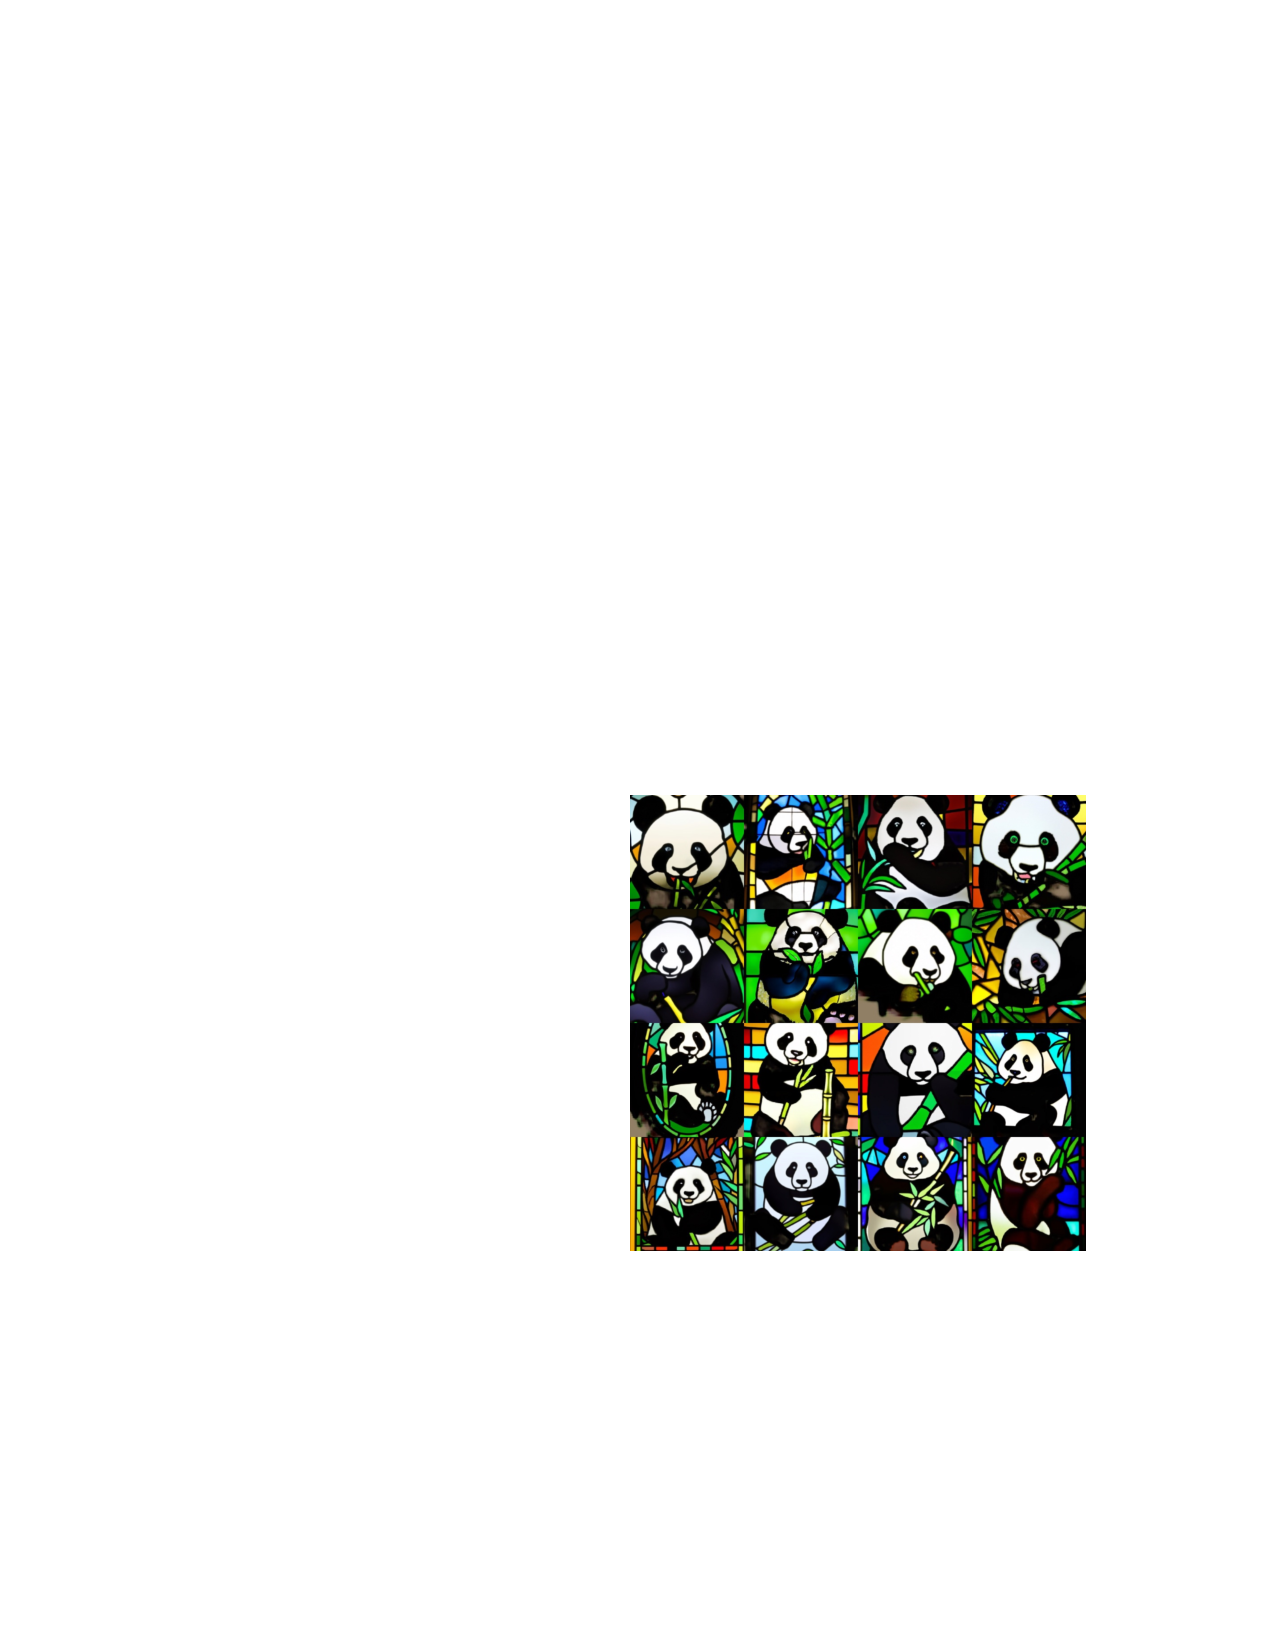
\includegraphics[width=0.45\textwidth]{images/dm/glide_guidance}
    \caption{Visualización del trade-off entre calidad y variedad al usar guidance. (Izquierda) modelo GLIDE incondicional. (Derecha) modelo GLIDE con classifier-free guidance, escala $\gamma=3.0$. Imagen obtenida desde \cite{nichol2022glidephotorealisticimagegeneration}.}
    \label{fig:glide}
\end{figure}

\paragraph{Classifier-free guidance}

Una limitación del enfoque anterior es que se vuelve necesario entrenar un clasificador $p_\theta(x_t|y)$ para cada tiempo $t\in\{0,\ldots,T\}$ del proceso de difusión ya que, al ser este un modelo discriminativo, nada garantiza poder clasificar bien para diferentes tiempos usando un único clasificador entrenado para $t=0$. Hacer este entrenamiento puede ser extremadamente costoso, por lo que en \cite{ho2022classifierfreediffusionguidance} proponen una alternativa que no requiere entrenar un clasificador separado, si no que lo entrenan a medida que se entrena el modelo de difusión. Para esto, vuelven a aplicar la regla de Bayes, pero ahora sobre el clasificador $p_\theta(y|x_t)$:

\begin{equation}
    \label{eq:guidance_discriminative}
    p_\theta(y|x_t) = \frac{p_\theta(x_t|y)p_\theta(y)}{p_\theta(x_t)}
    \implies
    \score{x_t}{p_\theta(y|x_t)} = \score{x_t}{p_\theta(x_t|y)} - \score{x_t}{p_\theta(x_t)}.
\end{equation}

Logrando obtener el término discriminativo necesario en \eqref{eq:classifier_guidance}. Otra observación que realizan en \cite{ho2022classifierfreediffusionguidance} es que todos los términos al lado derecho de \eqref{eq:guidance_discriminative} se pueden obtener si se entrena un modelo de difusión condicional $p_\theta(x|y)$ que permita entregar condiciones vacías para realizar generaciones incondicionales $p_\theta(x)$. Para esto:

\begin{itemize}
    \item Se entrena un modelo de difusión condicional $p_\theta(x_t|y)$, donde $y$ es una entrada adicional a la red neuronal.
    \item Durante el entrenamiento, de forma aleatoria se eligen iteraciones donde se entrena el modelo en modo incondicional. Esto es, se entrena $p_\theta(x|y)$ considerando como condición a un token especial $y=\emptyset$ que representa la ausencia de condición, simulando el aprendizaje de un modelo incondicional $p_\theta(x)$.
\end{itemize}

De esta forma, durante un único entrenamiento de un modelo de difusión condicional, es posible entrenar un modelo incondicional $p_\theta(x)$, lo que permite obtener la expresión $\score{x_t}{p_\theta(y|x_t)}$ necesaria en classifier-guidance sin haber entrenado un clasificador independiente. Por este motivo, esta técnica recibe el nombre de \textit{classifier-free guidance}.

Por otra parte, dado que es necesario entrenar un generador condicional para aplicar esta técnica, podría parecer que no se obtienen beneficios al aplicar classifier-free guidance (técnica que busca precisamente obtener un generador condicional). Sin embargo, al descomponer el score condicional, es posible aplicar el concepto de temperatura usado en classifier-guidance. En efecto, sustituyendo el lado derecho de \eqref{eq:guidance_discriminative} en \eqref{eq:guidance_temperature} se obtiene

\begin{align*}
    \score{x_t}{\tilde{p}_\theta(x_t|y)} &= \gamma\,\score{x_t}{p_\theta(y|x_t)} + \score{x_t}{p_\theta(x_t)}\\
    &= \gamma\parent{\score{x_t}{p_\theta(x_t|y)} - \score{x_t}{p_\theta(x_t)}}+ \score{x_t}{p_\theta(x_t)}\\
    &= (1-\gamma) \score{x_t}{p_\theta(x_t)} + \gamma\score{x_t}{p_\theta(x_t|y)}.
\end{align*}

Es decir, el score modificado que se debe usar para la generación condicional es una combinación baricéntrica (pero no necesariamente convexa) entre el score incondicional y el score condicional. En consecuencia, variando el parámetro $\gamma$ se obtienen 3 régimenes usuales:

\begin{itemize}
    \item \textbf{Temperatura infinita ($\gamma=0$):} se recupera el modelo incondicional $p_\theta(x)$ ya que la distribución condicional se vuelve uniforme (máxima entropía).
    \item \textbf{Temperatura unitaria ($\gamma=1$):} se obtiene el modelo condicional estándar.
    \item \textbf{Temperatura baja ($\gamma>1$):} la condición $y$ toma más relevancia, pudiendo controlar la influencia del prompt. Esto se observa en la \autoref{fig:glide}.
\end{itemize}

Por otra parte, al entrenar el modelo discriminativo $p(y|x_t)$ utilizando el mismo modelo de difusión, se suele obtener un clasificador mucho más robusto, por lo que la técnica de classifier-free guidance entrega mejores resultados que classifier-guidance. Más aún, en el trabajo de \cite{ho2022classifierfreediffusionguidance} muestran que con esta técnica, los modelos de difusión son estrictamente superiores que las GANs en cuanto a calidad y versatilidad de las muestras.

\subsubsection{Difusión en el espacio latente}

Una subfamilia importante dentro del grupo de los modelos de difusión son los \textit{latent diffusion models} (LDM). El trabajo más conocido en esta familia es \textit{Stable Diffusion}, cuya versión inicial se encuentra en \cite{rombach2022highresolution}. Este trabajo es un proyecto colaborativo de código abierto cuyos pesos (modelos entrenados) están disponibles para la comunidad.

La principal característica de este modelo es que trabaja en el espacio latente de las imágenes. Para esto, en \cite{rombach2022highresolution} primero entrenan un VAE para luego entrenar un modelo de difusión en el espacio latente de dicho VAE. Con esto, se consigue un entrenamiento más eficiente y se libera la opción de poder escalar el modelo a mayores resoluciones. El diagrama de la arquitectura del modelo \textit{Stable Diffusion} se puede ver en la \autoref{fig:dm/ldm_architecture}.

\insertimage{dm/ldm_architecture}{0.8}{Arquitectura del modelo \textit{Stable Diffusion}. El bloque rosado corresponde al VAE mientras que el bloque verde corresponde al modelo de difusión en el espacio latente. Para condicionar la generación, un embedding aprendido $\tau_\theta$ es inyectado a la U-Net mediante un mecanismo de \textit{cross-attention}. Imagen obtenida desde \cite{rombach2022highresolution}.}

Este modelo busca un espacio latente de menor dimensión\footnote{Al asumir que este espacio es de dimensión menor que la dimensión de los datos, implícitamente se está aceptando la \textit{manifold assumption}. En \cite{rombach2022highresolution} muestran empíricamente que la mayoría de los bits de una imagen digital corresponden a detalles imperceptibles.} que sea perceptualmente equivalente al espacio de los datos mediante el uso de un VAE. A diferencia de propuestas anteriores, aquí se entrena este modelo primero, sin considerar un modelo de difusión en particular. Esto permite reutilizar el VAE para entrenar distintos modelos de difusión, permitiendo explorar una mayor cantidad de variantes. Además, con el fin de evitar varianzas extremadamente largas en el espacio latente, los autores propusieron dos regularizaciones al VAE, que hoy se conocen como \textit{KL-reg} y \textit{VQ-reg}.

Por otra parte, la arquitectura del modelo \textit{Stable Diffusion} permite condicionar información externa $y$ de forma nativa (i.e., entrenando un modelo condicional) para poder realizar classifier-free guidance. Para esto, el modelo introduce un encoder especializado $\tau_\theta$, para así representar el condicionamiento $y$ mediante $\tau_\theta(y)$. Esta nueva representación es transmitida a cada capa de la U-Net mediante un mecanismo de \textit{cross-attention} (ver \cite{vaswani2023attention}), por lo que es necesario usar representaciones secuenciales:

\begin{itemize}
    \item $\mathcal{U}_i(z_t)\in\matrixspace{N,d_u^i}{\R}$ es una representación aplanada de la capa $i$ de la U-Net que realizará atención sobre la condición $\tau_\theta(y)$. Por lo tanto, en esa capa de atención será la secuencia que actúa como \textit{query}.
    \item $\tau_\theta(y)\in\matrixspace{M,d_\tau}{\R}$ actuará como el par \textit{key-value}. En el caso de que $y$ sea un texto, $\tau_\theta$ es el encoder de un transformer, $M$ es el largo de la secuencia y $d_\tau$ la dimensión de cada embedding. Es importante mencionar que el modelo $\tau_\theta$ se entrena al mismo tiempo que el modelo de difusión (\textit{Stable Diffusion} usa el enfoque $\epsilon-$prediction).
\end{itemize}

En la \autoref{fig:dm/stable_diffusion_cond} se ve una ilustración de este mecanismo de atención. Condicionando sobre imágenes, los autores de \cite{rombach2022highresolution} logran realizar síntesis semántica (creando imágenes realistas asociadas a un mapa semántico), super-resolución  e \textit{inpainting}\footnote{En términos generales, \textit{inpainting} consiste en llenar regiones de una imagen siguiendo una máscara. Esto sirve para reparar imágenes corruptas o sustituir partes con contenido no deseado en la imagen.}. En la \autoref{img:ldm_inpainting} se pueden ver ejemplos de estas técnicas.

\insertimage{dm/stable_diffusion_cond}{0.7}{Mecanismo de condicionamiento en el modelo \textit{Stable Diffusion}. La matriz $\tau_\theta$ es obtenida a partir de $y$. Un mecanismo de atención cruzada entre las distintas capas de la red y $\tau_\theta$ permite introducir la información de $y$ en la red. Imagen obtenida desde \cite{samarin2022powerdm}.}

\begin{figure}
    \centering
    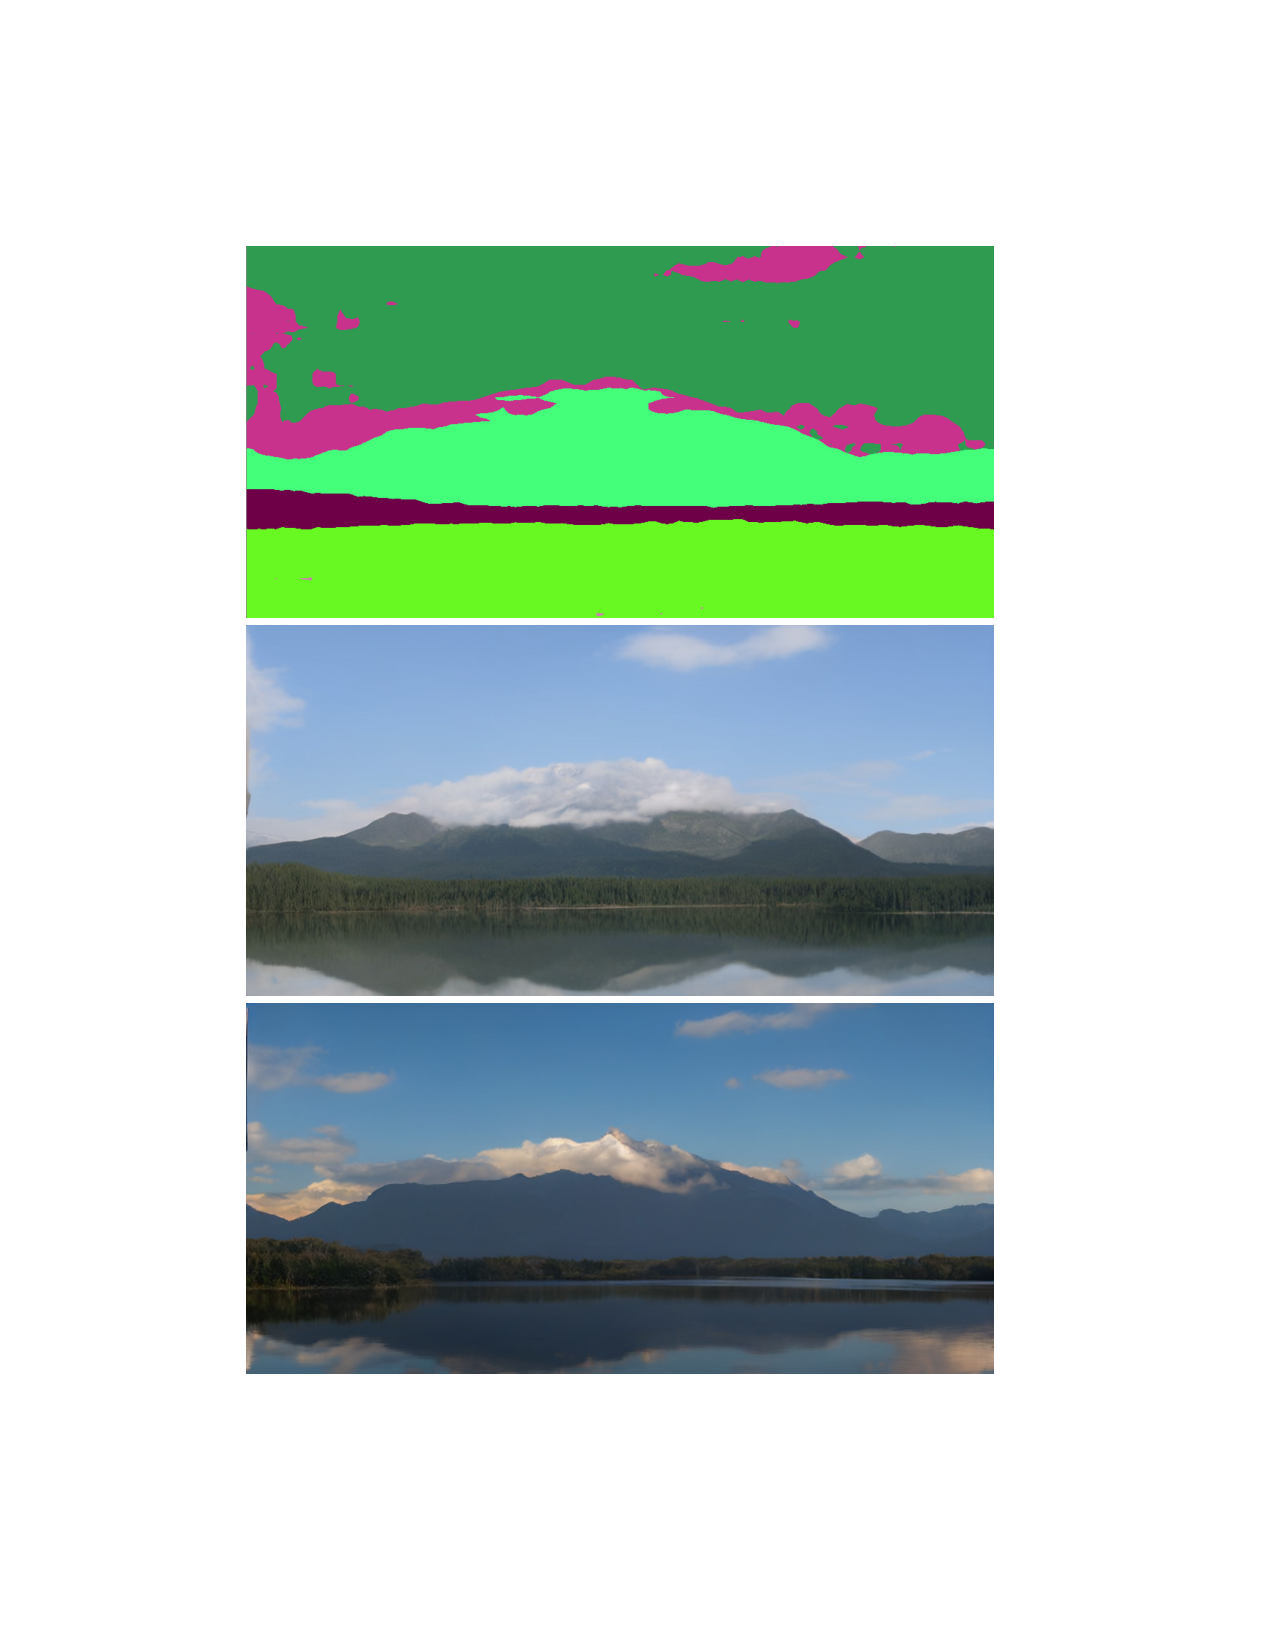
\includegraphics[width=0.45\textwidth]{images/dm/ldm_semantic_synthesis}
    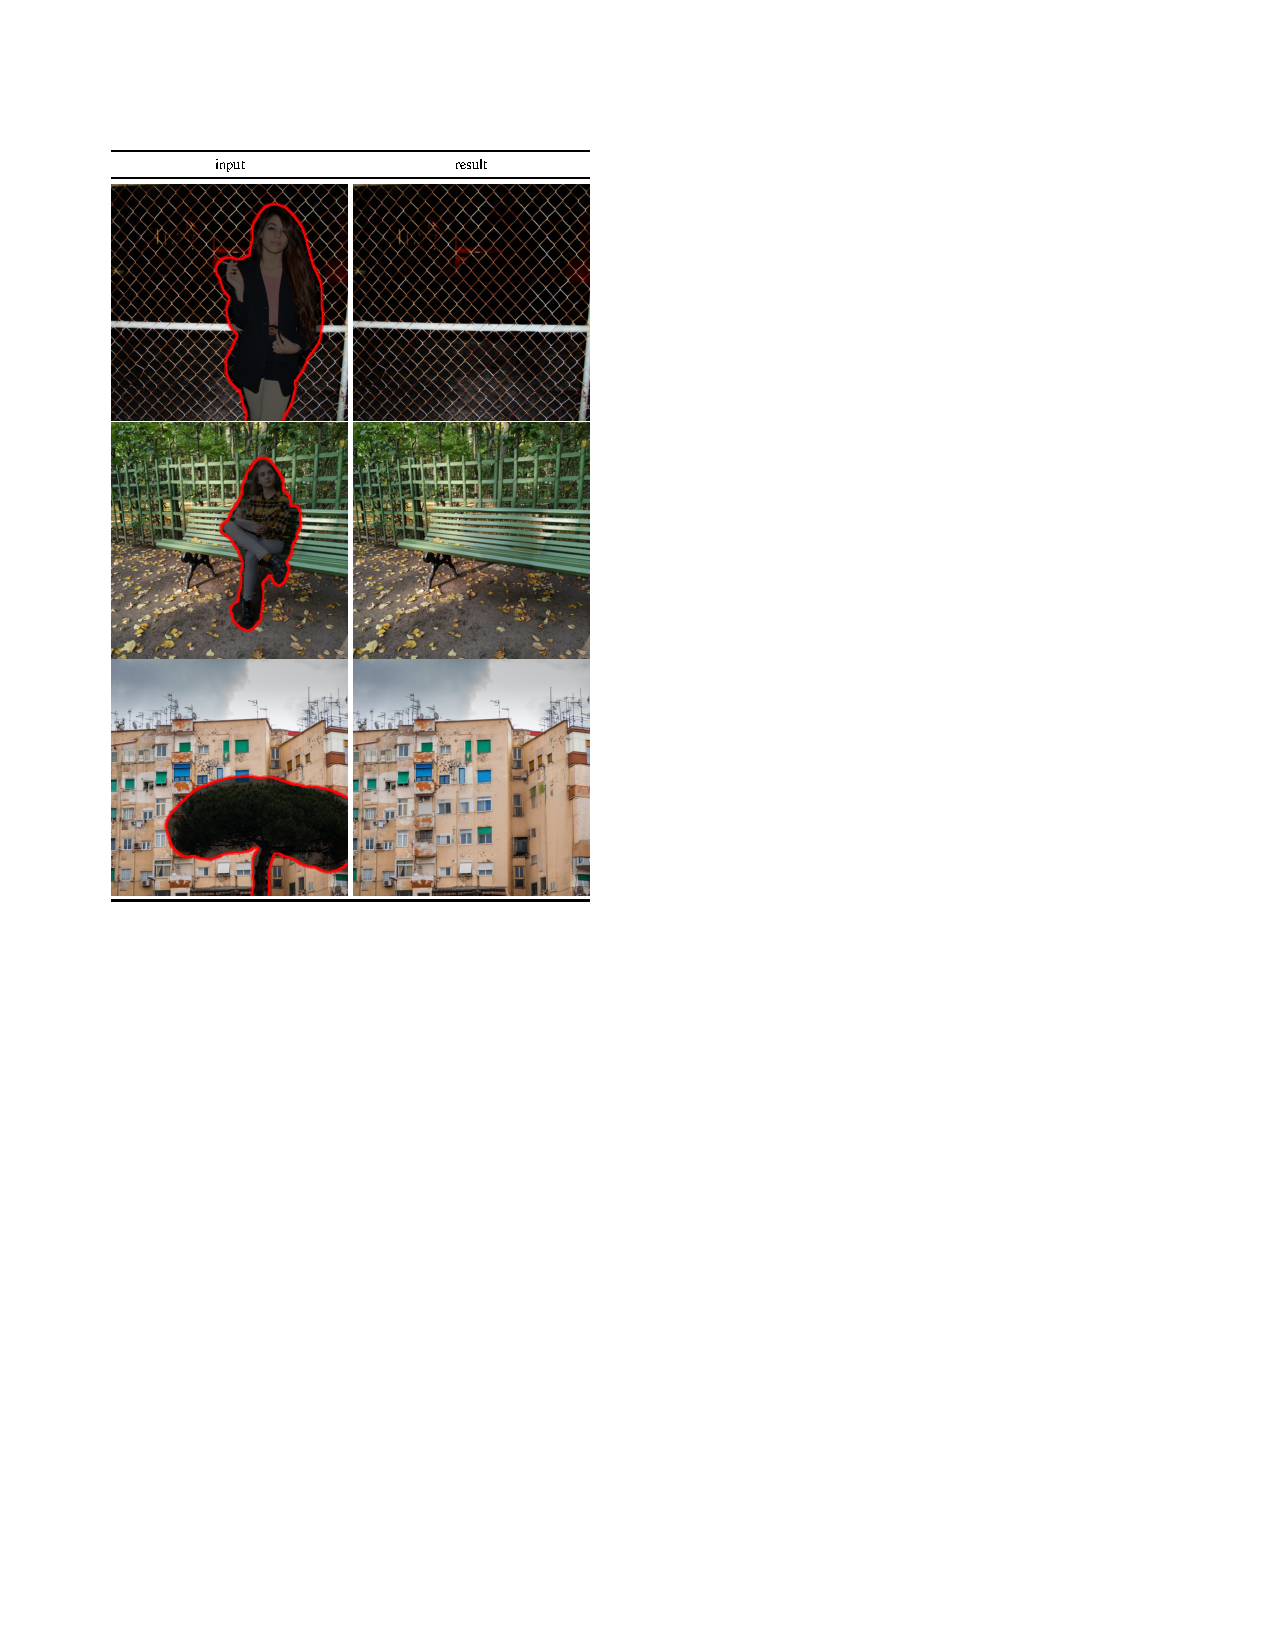
\includegraphics[width=0.45\textwidth]{images/dm/ldm_object_removal}
    \caption{(izquierda) generación condicionada a un mapa semántico. (derecha) eliminación de objetos mediante \textit{inpainting}. Imagen obtenida desde \cite{rombach2022highresolution}.}
    \label{img:ldm_inpainting}
\end{figure}

\section{Generalización a tiempo continuo}
\label{dm/continuous_dm}

En esta sección se revisará una generalización del modelo de difusión propuesto por \cite{ho2020denoising}, donde la cadena de Markov utilizada para los procesos de inyección de ruido y denoising será sustituida por un proceso estocástico a tiempo continuo. En consecuencia, en esta sección se utilizarán varios resultados acerca de ecuaciones diferenciales estocásticas (SDEs), los cuales se pueden encontrar en la \autoref{sde}. Esta formulación continua de los modelos de difusión será la que permitirá conectarlos con el problema del puente de Schrödinger en el \autoref{eot_sbp}. Además, este nuevo enfoque permite trabajar con diferentes procesos de inyección de ruido sobre un mismo marco teórico. Por otro lado, en \cite{song2021scorebased} notaron que, al ver el proceso de difusión en el continuo, es posible reducir la cantidad de iteraciones disminuyendo la precisión del \textit{solver} que se utilice para simular la SDE o la \textit{probability flow ODE} del proceso de generación.

Antes de introducir esta nueva formulación se revisará una formulación equivalente de los modelos de difusión a tiempo discreto donde se verá que aprender la media del proceso reverso es equivalente a aprender la derivada logarítmica de la distribución marginal $p_\theta(x_t)$ en un tiempo $t\in\{0,\ldots,T\}$, lo que permitirá, además, conectar los modelos de difusión con otra familia de modelos que al comienzo parecían independientes. Esta propiedad permitirá, posteriormente, aprender un proceso reverso a tiempo continuo gracias a un teorema importante del cálculo estocástico conocido como \textit{teorema de inversión de Anderson} (ver \autoref{teo:anderson}).

\subsection{Modelos generativos basados en score}
\label{dm/continuous_dm/score}

En esta subsección se revisará otra familia de modelos generativos denominada \textit{score-based models}. Si bien en un inicio este enfoque se propuso de manera independiente a los modelos de difusión, un trabajo posterior mostró que ambos paradigmas pueden ser vistos como un \textit{modelo de difusión} más general cuya dinámica de difusión y denoising viene dada por una SDE. El concepto principal de este tipo de modelos es el siguiente:

\begin{defn}[función de score]
    \label{defn:score}
    Dada una distribución de probabilidad con densidad $p$, se define la \textit{función de score}\footnote{A esta función también se le denomina \textit{score de Hyvärinen} o \textit{score de Stein}, para diferenciarla de la función score usada en la definición de la \textit{información de Fisher}. En esta última, el gradiente es tomado con respecto a los parámetros del modelo, mientras que aquí se está considerando el gradiente con respecto a la entrada.} de dicha distribución, $\operatorname{score}_p:\R^d\to\R^d$, como la derivada logarítmica de su densidad:

\begin{equation*}
    \operatorname{score}_p(x) := \nabla_x \log p(x).
\end{equation*}
\end{defn}

Los modelos que buscan aprender la función de score en vez de aprender directamente la densidad $p$ (que es lo que hacen los modelos basados en verosimilitud) se denominan \textit{modelos basados en score} y pueden ser vistos como una variante de los modelos basados en energía \cite{song2021trainenergybasedmodels}. Es importante notar que una función de score define totalmente una única función verosimilitud $\log p(x)$. En efecto, si $\nabla_x \log p_1(x) = \nabla_x \log p_2(x)$ entonces, por el teorema fundamental del cálculo, $\log p_1(x) = \log p_2(x)+c$, donde necesariamente $c=0$ cuando $p_1$ y $p_2$ son densidades de probabilidad en $\R^d$, en efecto:

\begin{equation*}
    \log p_1(x) = \log p_2(x)+c \implies \int_{\R^d} e^{\log p_1(x)} \d x = \int_{\R^d} e^{\log p_2(x)+c}\d x \implies 1 = e^c \implies c = 0 .
\end{equation*}

De esta forma, una función de score caracteriza totalmente a su densidad de probabilidad asociada.

\subsubsection{Modelo de score matching}

Para comenzar el estudio de los modelos badados en score, se revisará el modelo generativo de \textit{score matching}, el cual consiste en aprender la función de score de una distribución $\ptrue$ aprovechando el hecho de que los modelos basados en redes neuronales se pueden derivar fácilmente mediante diferenciación automática.

Dada una densidad desconocida $\ptrue$ y un modelo paramétrico $s_\theta$ que busque aprender el score de $\ptrue$, la función objetivo natural en este caso es la divergencia de Fisher entre la densidad real $\ptrue$ y la densidad aprendida a partir de $s_\theta$, $p_\theta$:

\begin{align*}
    \DF{\ptrue}{p_\theta} := & \frac{1}{2}\E{x\sim\ptrue(x)}{\norm{\nabla_x\log \ptrue(x) - \nabla_x\log p_\theta(x)}^2} \\
    =                        & \frac{1}{2}\E{x\sim\ptrue(x)}{\norm{\nabla_x\log \ptrue(x) - s_\theta(x)}^2} ,
\end{align*}

donde $p_\theta$ es la densidad asociada al score $s_\theta$. Al igual que antes, la esperanza es aproximada según la distribución empírica asociada a un conjunto de muestras de entrenamiento $(x^k)_{k=1}^n$ proveniente de $\ptrue$. Si bien el score real $\nabla_x\log \ptrue(x)$ no es conocido, en \cite{hyvarinen2005estimation} prueban que la divergencia de Fisher es equivalente al siguiente objetivo:

\begin{prop}[divergencia de Fisher para score matching]
    Dada una densidad desconocida $\ptrue$ y otra densidad $p_\theta$ con función de score $s_\theta$ conocida, se tiene que:

    \begin{equation*}
        \label{eq:sm_objective}
        \DF{\ptrue}{p_\theta} =
        \E{x\sim\ptrue(x)}{\frac{1}{2}\norm{s_\theta(x)}^2 + \trace{\nabla_x s_\theta(x)}} + \cte ,
    \end{equation*}

    donde $\trace{\cdot}$ es el operador traza y $\nabla_x s_\theta(x)\in\matrixspace{d,d}{\R}$ es la matriz jacobiana de $s_\theta$ (evaluada en $x$).
\end{prop}

De esta forma se obtiene una función de pérdida tratable\footnote{Dado que la función de score $s_\theta$ es modelada mediante una red neuronal, sus derivadas pueden ser encontradas mediante diferenciación automática. En el archivo \texttt{sgm.ipynb} se implementa un modelo con esta función objetivo.}, lo que permite aprender la función de score de $\ptrue$ dado un conjunto de muestras para el entrenamiento. Este método se conoce en la literatura como \textit{score-matching} (SM).

Una vez aprendido un modelo de score, lo único que queda pendiente es ver cómo generar muestras a partir de $p_\theta$ teniendo únicamente la función de score $s_\theta$. Para esto, es usual usar un algoritmo denominado \textit{Langeving sampling} o \textit{Langeving Monte Carlo} (LMC), donde este último nombre se debe a que este algoritmo puede interpretarse como un caso particular de una variante del método de MCMC, denominada \textit{Hamiltonian Monte Carlo} (HMC). Para estas variantes ver, por ejemplo, \cite{pml2Book}.

La idea del algoritmo de Langevin sampling es simular un proceso dinámico aleatorio específico, $x=(x_t)_{t\geq 0}$,  del cual se sabe que para tiempos de simulación $t\gg 1$ muy largos, la distribución marginal de $x_t$, $p(x_t)$, es precisamente la distribución que se quiere simular. Un proceso que tiene esta propiedad es conocido como dinámica de Langevin, cuya SDE (ver \autoref{sde}) es

\begin{equation}
    \label{eq:langevin_sde}
    \d x_t = \frac{1}{2}\nabla_{x_t} \log \pi(x_t) \d t + \d w ,
\end{equation}

donde $\pi(x)$ es alguna función de densidad de la que se quiere generar muestras. La siguiente proposición indica que este proceso estocástico tiene la propiedad buscada:

\begin{prop}[distribución estacionaria de la dinámica de Langevin]
    Si $p(x_t)$ denota la densidad marginal en tiempo $t$ del proceso estocástico $(x_t)_{t\geq 1}$ que resuelve la SDE \eqref{eq:langevin_sde}, entonces $\pi$ es la distribución estacionaria del proceso estocástico $x$, es decir, $p(x_t)\to \pi(x_t)$ cuando $t\to\infty$.
\end{prop}

\begin{proof}
    Por simplicidad, se demostrará el resultado en el caso unidimensional ($d=1$). En este caso, la SDE asociada al proceso estocástico $x=(x_t)_{t\geq 1}$ toma la forma

    \begin{equation}
        \label{eq:langevin_sde_1d}
        \d x_t = \frac{1}{2}\parent{\log \pi}'(x_t) \d t + \d w .
    \end{equation}
    
    Por otra parte, si $p(x,t)=p(x_t)$ es la densidad marginal en tiempo $t$, entonces $p(x,t)$ cumple ecuación de Fokker-Planck (ver \autoref{teo:fokker_planck}) asociada a la SDE \eqref{eq:langevin_sde_1d}. Denotando las derivadas como subíndices:

    \begin{align*}
        p_x
        = -\frac{\partial}{\partial x} \parent{\frac{1}{2}\parent{\log \pi}' p} + \frac{1}{2} \frac{\partial^2}{\partial x^2} \parent{1^2 p}
        = -\frac{1}{2}\parent{\parent{\log\pi}''p+\parent{\log\pi}'p_x} + \frac{1}{2}p_{xx}.
    \end{align*}

    Tomando $p_x=0$ (donde la densidad marginal ya no cambia) se obtiene la SDE de la distribución estacionaria:

    \begin{align*}
        &p_{xx} - \parent{\log\pi}'p' - \parent{\log\pi}'' p = 0\\
        &p_{xx}-\frac{\pi'}{\pi}p' - \frac{\pi''\pi-\parent{\pi'}^2}{\pi^2}p = 0.
    \end{align*}

    Se verá que la densidad $p(x,t)=\pi(x)$ satisface esta ecuación:

    \begin{equation*}
        \pi_{xx}-\frac{\pi'}{\pi}\pi' - \frac{\pi''\pi-\parent{\pi'}^2}{\pi^2}\pi
        = \frac{\pi''\pi-\parent{\pi'}^2}{\pi^2}\pi - \frac{\pi''\pi-\parent{\pi'}^2}{\pi^2}\pi = 0 .
    \end{equation*}

    Por lo tanto, $\pi$ es la distribución estacionaria de la dinámica de Langevin.
\end{proof}

El resultado anterior nos garantiza que simular el proceso estocástico asociado a la SDE \eqref{eq:langevin_sde} permite obtener una muestra desde la distribución $\pi$ si la simulación se realiza hasta un tiempo $T\gg 1$ lo suficientemente grande\footnote{En rigor, la distribución estacionaria se alcanza en un horizonte de tiempo infinito, por lo que siempre se obtienen muestras de una distribución $p(x_t)$ cercana pero no igual a la distribución estacionaria. El problema del puente de Schrödinger estudiado en el \autoref{eot_sbp} soluciona este problema.}. Aplicando este método para generar muestras desde una densidad $p_\theta$ de la cual se conoce su función de score $s_\theta=\log p_\theta$, se obtiene el procedimiento de generación de muestras para un método basado en score, el cual se conoce como Langevin sampling y se detalla en el \autoref{alg:langevin}, donde la SDE \eqref{eq:langevin_sde} es simulada utilizando el algoritmo de Euler-Maruyama (ver \autoref{alg:euler-maruyama}).

\begin{algorithm}
    \caption{Langevin sampling}
    \label{alg:langevin}
    \begin{algorithmic}[1]
        \Require Distribución inicial $p_0$, cantidad de iteraciones $T$ y largo de paso $\epsilon$.
        \Require Función de score aprendida $s(x) = \nabla_x \log p(x)$
        \State Generar iteración inicial $x_0\sim p_0(x_0)$.
        \For{$t$ desde 1 a hasta $T$}
        \State Generar $z_t\sim \gaussian{0}{\identity{d}}$.
        \State $x_t\gets x_{t-1} + \frac{\epsilon}{2}s(x_{t-1}) + \sqrt{\epsilon} z_t$
        \EndFor
        \State\Return $x_T$
    \end{algorithmic}
\end{algorithm}

El \autoref{alg:langevin} puede verse como un método de gradiente ascendente perturbado que dirige $x_t$ hacia los máximos de $p_\theta$. Al agregar aleatoriedad mediante el ruido $z_t$ se está garantizando que $x=(x_t)_{t=1}^T$ no colapse hacia alguna de las modas (máximos locales) de $p_\theta$. En el archivo \texttt{sgm.ipynb} se encuentra implementado este modelo para un dataset de juguete.

\subsubsection{Score matching mediante la inyección de ruido}

Una de las principales limitaciones del enfoque anterior es el tiempo cuadrático que toma computar el término $\trace{\operatorname{J}_x s_\theta(x)}$ durante el entrenamiento en \eqref{eq:sm_objective} ya que se vuelve intratable en altas dimensiones. Para evitar computar este término directamente, se han propuesto diferentes variantes de score-matching como \textit{sliced score matching} (SSM\footnote{No confudir con los \textit{state space models} \cite{gu2022efficientlymodelinglongsequences}, los cuales no tienen relación directa con los modelos basados en score.}) en \cite{song2019sliced} y \textit{Denoising score matching} (DSM) en \cite{DSM}. Este último enfoque realiza score matching sobre los datos perturbados por la inyección de un ruido aditivo $\tilde{x} = x+\epsilon$, estimando el score de $q(\tilde{x})=\int q(\tilde{x}|x)\ptrue(x)\d x$ en vez de estimar directamente el score de $\ptrue$. Con esto, en \cite{DSM} muestran que la divergencia de Fisher toma la siguiente forma:

\begin{prop}[divergencia de Fisher para DSM]
    \label{prop:fisher_dsm}
    Dado un modelo paramétrico $p_\theta$ con función de score $s_\theta$ conocida, si $p_\theta$ busca aproximar una densidad desconocida $q=\int q(\cdot|x)\ptrue(x)\d x$, se tiene que:

    \begin{align*}
        \DF{q}{p_\theta} & = \frac{1}{2}\E{\tilde{x}\sim q(\tilde{x})}{\norm{\nabla_{\tilde{x}}\log q(\tilde{x}) - s_\theta(\tilde{x})}^2}                             \\
                         & = \frac{1}{2}\E{x\sim\ptrue(x),\,\tilde{x}\sim q(\tilde{x}|x)}{\norm{\nabla_{\tilde{x}}\log q(\tilde{x}|x) - s_\theta(\tilde{x})}^2} + \cte .
    \end{align*}
\end{prop}

Dado que se considera un kernel de perturbación gaussiano $q(\tilde{x}|x) \sim \gaussian{x}{\sigma^2 \identity{d}}$, el score $\nabla_{\tilde{x}}\log q(\tilde{x}|x)$ se puede obtener en forma cerrada y la función objetivo se simplifica a una cantidad tratable:

\begin{equation}
    \label{eq:fisher_dsm}
    \DF{q}{p_\theta} = \frac{1}{2}\E{x\sim\ptrue(x),\,\tilde{x}\sim \gaussian{x}{\sigma^2 \identity{d}}}{\norm{\frac{x-\tilde{x}}{\sigma^2} - s_\theta(\tilde{x})}^2} .
\end{equation}

De esta forma, estimando el score sobre los datos perturbados se evita la dificultad de computar $\trace{\operatorname{J}_x s_\theta(x)}$ en \eqref{eq:sm_objective} y, si bien el modelo está aprendiendo el score de $q(\tilde{x})$, se puede considerar que $q\approx\ptrue$ cuando $\sigma^2$ es suficientemente pequeño.

Esta técnica, conocida como \textit{denoising score matching} (DSM), también soluciona otros problemas observados en el modelo SM original:

\begin{itemize}
    \item Considerando la \textit{manifold assumption}, el score $\score{x}{\ptrue(x)}$ está indefinido en gran parte del dominio de $\ptrue$ ya que el soporte de $\ptrue$ está confinado en una variedad de dimensión estrictamente menor. Más aún, esta hipótesis implica que la medida de probabilidad real asociada a los datos de entrenamiento, $\mu_{\text{true}}$, no debería poseer una función de densidad $\ptrue$ (ver \autoref{measure_theory/density}). Al usar una perturbación gaussiana, el soporte vuelve a ser todo $\R^d$.
    \item Este kernel de perturbación asegura que la densidad condicional $q(\tilde{x}|x)$ sea diferenciable, lo cual no es necesariamente cierto al tratar directamente con $\ptrue$.
\end{itemize}

En el archivo \texttt{sgm.ipynb} se encuentra una implementación minimal de este tipo de modelos donde se puede comparar \eqref{eq:fisher_dsm} con la función objetivo \eqref{eq:sm_objective}.

Por otra parte, si bien la técnica presentada en \cite{DSM} estabiliza el entrenamiento, un trabajo posterior muestra algunas de sus limitaciones y propone hacer DSM utilizando distintos niveles de ruido. En particular, los problemas adicionales que reconocen en \cite{song2020generative} son los siguientes:

\begin{itemize}
    \item Considerando que las muestras de entrenamiento fueron generadas directamente desde $\ptrue$, es altamente problable no tener muestras de entrenamiento en regiones de baja densidad. En consecuencia, dado que la esperanza de la divergencia de Fisher en \eqref{eq:fisher_dsm} es aproximada mediante la distribución empírica, la función de score aprendida $s_\theta$ no será correcta en zonas de baja densidad. Esto puede observarse en la \autoref{fig:dm/sgm_low_density}.

          \insertimage{dm/sgm_low_density}{0.6}{Campo vectorial de la función de score real (izquierda) y de la función de score aprendida (derecha) para una mixtura gaussiana. El mapa de calor está asociado a la densidad de la mixtura y los rectángulos muestran las zonas donde la predicción del score es cercana a la real. Se observa que la predicción solo es precisa alrededor de las modas de la mixtura.}

    \item Dada una mixtura $p_{\text{mixture}} = \pi p_1 + (1-\pi) p_2$, donde $p_1$ y $p_2$ son densidades con soporte disjunto, su score vendrá dado por:

          \begin{equation*}
              \score{x}{p_{\text{mixture}}}(x) = \begin{cases}
                  \nabla_x (\log \pi + \log p_1(x)) = \nabla_x\log p_1(x),     &\text{si } x\in\supp{p_1} \\
                  \nabla_x (\log (1-\pi) + \log p_2(x)) = \nabla_x\log p_2(x), &\text{si } x\in\supp{p_2} .
              \end{cases}
          \end{equation*}

          Por lo tanto, el score de la mixtura no depende de $\pi$ y la dinámica de Langevin no podrá generar muestras respetando los ponderadores de la mixtura, dándole igual probabilidad a muestras generadas desde $p_1$ o $p_2$. Si bien al agregar ruido gaussiano el soporte pasa a ser todo $\R^d$, el fenómeno se sigue observando cuando se intentan conectar dos regiones separadas por zonas de baja densidad, donde la dinámica de Langevin requerirá más iteraciones para converger. Este problema se observa en la \autoref{fig:dm/langevin} y en la \autoref{fig:dm/sgm_mixture_sampling} (centro).
\end{itemize}

\begin{figure}
    \centering
    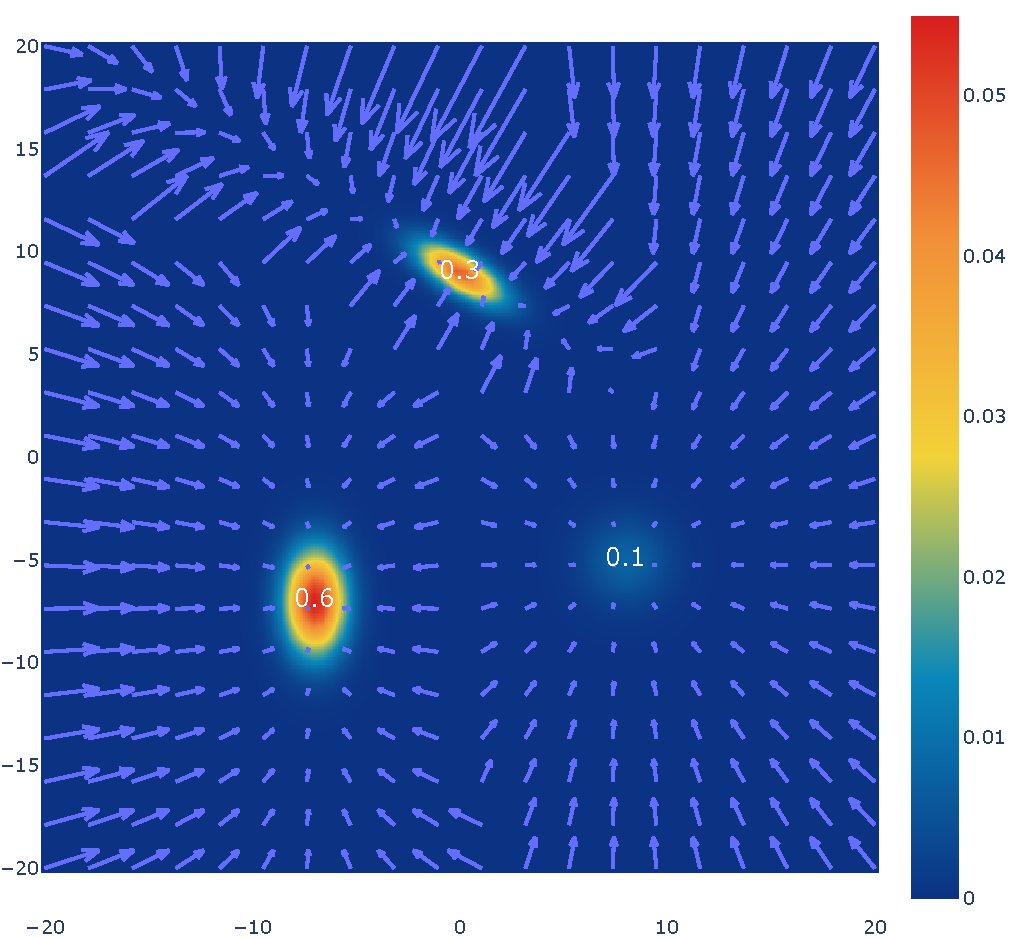
\includegraphics[width=0.45\textwidth]{images/dm/langevin_gmm}
    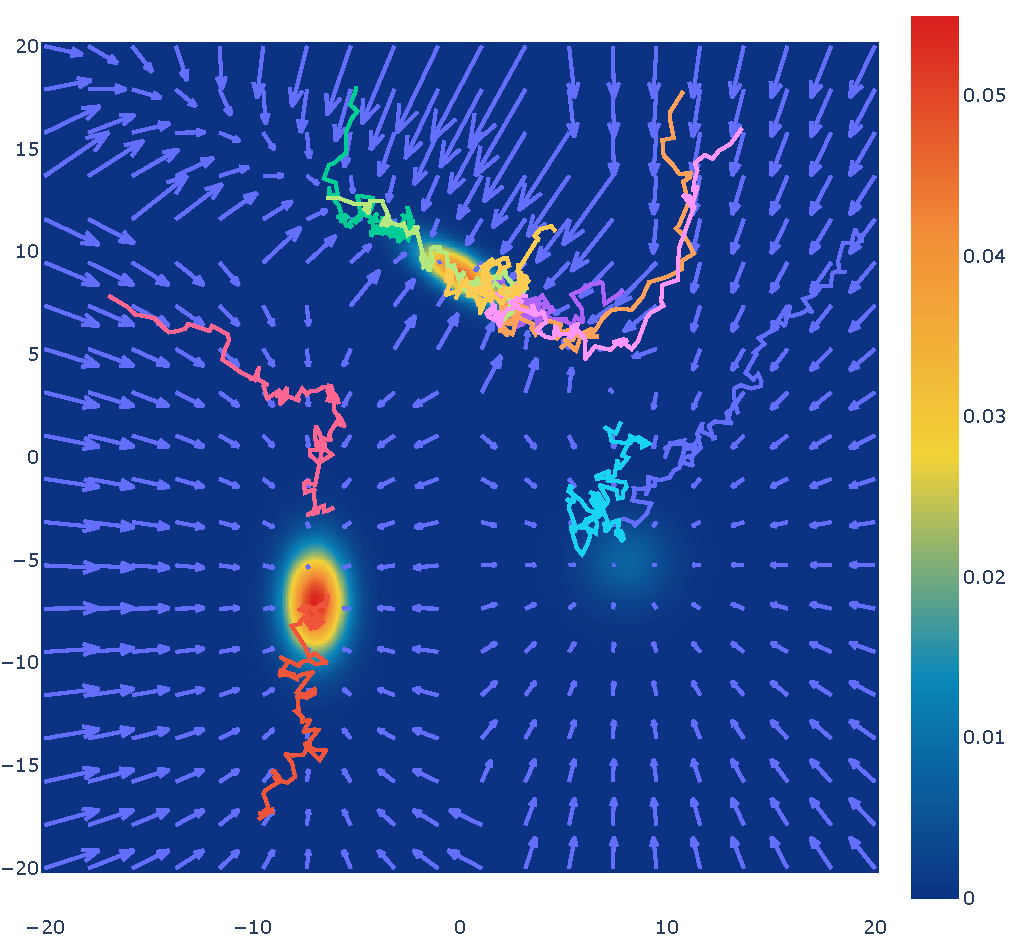
\includegraphics[width=0.45\textwidth]{images/dm/langevin_gmm_samples}
    \caption{Muestras generadas a partir de una mixtura gaussiana utilizando la dinámica de Langevin dada en el \autoref{alg:langevin}. El mapa de calor indica la densidad de la mixtura en cada punto del plano y las curvas muestran la trayectoria seguida por el proceso de generación $(x_t)_{t=1}^T$. Se observa que la dinámica de Langevin no es capaz de respetar los priors de cada componente de la mixtura, donde se esperaría que la componente con mayor relevancia (con prior de clase $0.6$) tenga una mayor cantidad de muestras generadas. Esta simulación se encuentra en el archivo \texttt{langevin.ipynb}.}
    \label{fig:dm/langevin}
\end{figure}

\insertimage{dm/sgm_mixture_sampling}{0.9}{(izquierda) muestras de entrenamiento generadas a partir de la mixtura de la \autoref{fig:dm/sgm_low_density}. (centro) muestras generadas mediante DSM con la dinámica de Langevin usual. (derecha) muestras generadas con la dinámica de Langevin propuesta por \cite{song2020generative}.}

Para atacar estos problemas, los autores de \cite{song2020generative} proponen dos mejoras. En primer lugar, continúan usando el enfoque de DSM ,pero utilizando distintos niveles de ruido. Por un lado, al usar un ruido de alta varianza se soluciona el problema de tener regiones de muy baja densidad y la aproximación del score puede ser más exacta, pero la distribución aprendida se aleja de la distribución buscada $\ptrue$. Con esta observación, los autores proponen utilizar una secuencia creciente\footnote{Originalmente, en \cite{song2020generative}, se define la secuencia en orden decreciente. Aquí se considerará en orden creciente para seguir el mismo orden que el modelo DDPM.} de niveles de ruidos $(\sigma_k)_{k=1}^L\subset\R_{++}$, cada uno asociado a un kernel de perturbación $q_{\sigma_k}$ definido, al igual que antes, como un ruido aditivo $x\mapsto x+z,\,z\sim\gaussian{0}{\sigma_k^2 \identity{d}}$. Los autores proponen usar una secuencia geométrica de niveles de ruido tal que $\sigma_1$ sea lo suficientemente pequeño para que $q_{\sigma_1}\approx\ptrue$, y $\sigma_L$ sea lo suficientemente grande para que $q_{\sigma_L}\approx\gaussian{0}{\sigma_L\identity{d}}$ y que además se logre mitigar el problema de las zonas de baja densidad.

De esta forma, para cada $\sigma\in(\sigma_k)_{k=1}^L$ se entrena un modelo de score $s_\theta(x,\sigma)$ que aproxime a $\nabla_x \log q_\sigma(x)$. Con esto, se tendrá una función de score-matching (ver \eqref{eq:fisher_dsm}) para cada nivel de ruido. La función objetivo final será un promedio ponderado de las pérdidas individuales\footnote{Se puede justificar el mejor desempeño de este modelo sobre el original considerando el promedio como un \textit{ensemble} (ver \textit{bagging} en \cite{bishop2006pattern}).}:

\begin{align}
    l_\sigma(\theta) : & = \frac{1}{2}\E{x\sim\ptrue,\,\tilde{x}\sim \gaussian{x}{\sigma^2 \identity{d}}}{\norm{\frac{x-\tilde{x}}{\sigma^2} - s_\theta(\tilde{x}, \sigma)}^2},\quad \forall\sigma\in (\sigma_k)_{k=1}^L\nonumber \\
    L(\theta)          & = \frac{1}{L} \sum_{k=1}^L \lambda(\sigma_k) l_{\sigma_k}(\theta)\label{eq:dsm_loss}.
\end{align}

Si bien se podrían utilizar modelos de score $s_\theta$ independientes para cada nivel de ruido $\sigma$, es usual considerar una única red neuronal $s_\theta(x,\sigma)$ entrenada de forma conjunta para todos los niveles de ruido. En \cite{song2020generative} le llaman a esta red \textit{noise conditional score network} (NCSN).

Para la elección del ponderador $\lambda(\sigma)$, los autores notaron empíricamente que, en el óptimo, $\norm{s_\theta(\cdot, \sigma)}\propto \sigma^{-1}$, por lo que tomando $\lambda(\sigma) = \sigma^2$, el término $\lambda(\sigma_k) l_{\sigma_k}(\theta)$ se vuelve independiente de $\sigma$ y así, ningún sumando de $L$ gana o pierde relevancia únicamente por el nivel de ruido $\sigma$.

En segundo lugar, para la generación de muestras, los autores de \cite{song2020generative} proponen una modificación al algoritmo de Langevin descrito en el \autoref{alg:langevin}, donde ahora computan una cadena de Langevin $(x_t)_{t=1}^T$ para cada uno de los niveles de ruido (de forma descendente en la cantidad de ruido), y el estado inicial de la cadena para el ruido $\sigma_k$ viene dado por el estado final de la cadena para el ruido $\sigma_{k+1}$. El \autoref{alg:annealed_langevin} detalla el procedimiento.

\begin{algorithm}
    \caption{Annealed Langevin sampling}
    \label{alg:annealed_langevin}
    \begin{algorithmic}[1]
        \Require Niveles de ruido $(\sigma_k)_{k=1}^L$ usandos durante el entrenamiento.
        \Require Distribución inicial $\pi$, cantidad de iteraciones $T$ por nivel de ruido y largo de paso $\epsilon$.
        \Require Modelo $s_\theta(\cdot,\cdot)$ ya entrenado.
        \State Generar $x_0\sim \pi(x_0)$.
        \For{$k$ desde $L$ hasta 1}
        \State $\epsilon_k \gets \epsilon \frac{\sigma_k^2}{\sigma_L^2}$  \Comment{Largo de paso adaptado para el nivel de ruido.}
        \For{$t$ desde 1 hasta $T$}
        \State Generar $z_t\sim \gaussian{0}{\identity{d}}$.
        \State $x_t\gets x_{t-1} + \frac{\epsilon_k}{2}s_\theta(x_{t-1},\sigma_k) + \sqrt{\epsilon_i} z_t$
        \EndFor
        \State $x_0\gets x_T$
        \EndFor
        \State\Return $x_T$
    \end{algorithmic}
\end{algorithm}

Si bien esta variante de DSM recibe distintos nombres en la literatura, aquí se le seguirá denominando simplemente DSM ya que se ha vuelto la variante predominante en esta familia de modelos y serán los que se conectarán con el modelo DDPM. En el archivo \texttt{sgm.ipynb} hay una implementación de SM y DSM.

\subsubsection{DDPM como modelo basado en score}

Hasta el momento, los modelos basados en score han sido trabajados como modelos totalmente independientes de los modelos de difusión descritos en la \autoref{dm/discrete_dm/formulation}. En este apartado se mostrará que los modelos de difusión pueden ser formulados como un modelo DSM con ciertos niveles de ruido. Posteriormente, en la \autoref{dm/continuous_dm/sde_dm} se verá que ambos modelos corresponden a una familia de modelos de difusión más general, donde el proceso forward vendrá dado por un proceso estocástico a tiempo continuo. Por otra parte, es importante recordar que la técnica de \textit{guidance} para la generación condicional es posible gracias el hecho de poder escribir el modelo DDPM como un modelo basado en score.

Para un modelo de difusión, en la \autoref{dm/discrete_dm/formulation} se mostró que lo único que se necesita para invertir el proceso de inyección de ruido mediante transiciones $p_\theta(x_{t-1}|x_t)\sim\gaussian{\mu_\theta(x_t,t)}{\sigma_q^2(t)\identity{d}}$ es aprender una función de media $\mu_\theta(x_t,t)$ que aproxime a la media de $q(x_{t-1}|x_t,x_0)$, $\mu_q(x_0,x_t,t)$ (ver \eqref{eq:conditional_backward_params}). Para esto, se estudiaron distintas formulaciones equivalentes:

\begin{itemize}
    \item Aprender $\mu_q(x_0,x_t,t)$ directamente mediante un modelo $\mu_\theta(x_t,t)$.
    \item Aprender la muestra $x_0$ que generó $x_t$ en la etapa $t$ mediante un modelo $x_\theta(x_t,t)$.
    \item Aprender el ruido $\epsilon$ inyectado a $x_0$ en la etapa $t$ mediante un modelo $\epsilon_\theta(x_t,t)$.
\end{itemize}

Para ver que un modelo de difusión se puede escribir como un modelo basado en score, se deducirá una cuarta forma de formular el problema de optimización, donde ahora un modelo paramétrico $s_\theta(x_t,t)$ tendrá que aprender el score $\nabla_x\log p(x_t)$ para obtener un modelo $\mu_\theta(x_t,t)$ para aprender la función de media $\mu_q(x_t,t,t)$. Para introducir la función de score en el modelo se utilizará el siguiente resultado:

\begin{teo}[fórmula de Tweedie, caso gaussiano]
    Sea $p(z|\mu)\sim\gaussian{\mu}{\Sigma}$, con $\mu\sim p(\mu)$ una distribución desconocida y $\Sigma$ un parámetro fijo y conocido. Dada una muestra $z\sim p(z)= \int p(z|\mu) p(\mu)\d\mu$, entonces:

    \begin{equation*}
        \E{p(\mu|z)}{\mu} = z + \Sigma \cdot\hspace{-.3cm} \underbrace{\nabla_z \log p(z).}_{\text{corrección de Bayes}} 
    \end{equation*}
\end{teo}

\begin{proof}
    Usando que $\int z\,p(\mu|z) = z\int p(\mu|z)=z$ y por teorema de Bayes:

    \begin{equation*}
        \E{p(\mu|z)}{\mu} = \int \mu\, p(\mu|z)d\mu = z - \int (z-\mu)p(\mu|z) d\mu = z - \int (z-\mu)\frac{p(z|\mu)p(\mu)}{p(z)} d\mu .
    \end{equation*}

    Notando que $\score{z}{p(z|\mu)} = -\Sigma^{-1} (z-\mu)$, el integrando se escribe como:

    \begin{equation*}
        (z-\mu)\frac{p(z|\mu)p(\mu)}{p(z)} = -\Sigma \score{z}{p(z|\mu)} \frac{p(z|\mu)p(\mu)}{p(z)} = -\Sigma \frac{\nabla_z p(z|\mu)}{p(z|\mu)} \frac{p(z|\mu)p(\mu)}{p(z)} = -\Sigma \frac{\nabla_z p(z,\mu)}{p(z)} .
    \end{equation*}

    Por lo tanto, por regla de de integración de Leibniz:

    \begin{equation*}
        \E{p(\mu|z)}{\mu|z} = z + \Sigma \frac{\int \nabla_z p(z,\mu)d\mu}{p(z)} = z + \Sigma \frac{\nabla_z \int p(z,\mu)d\mu}{p(z)} = z + \Sigma \frac{\nabla_z p(z)}{p(z)} .
    \end{equation*}

    Donde el cociente es precisamente el score de $p(z)$.
\end{proof}

Este resultado busca corregir la estimación empírica de la media real $\mu$\footnote{Recordar que el estimador de máxima verosimilitud de la media es la media empírica, que en este caso es $z$.} mediante un desplazamiento según el score de $z$. Esta corrección es importante en casos donde la muestra $z$ puede ser un outlier, en cuyo caso el score $\score{z}{p(z)}$ buscará desplazar la estimación hacia el centro.

En la \autoref{prop:epsilon_prediction} se usó que $q(x_t|x_0)\sim\gaussian{\sqrt{\overline{\alpha}_t}x_0}{(1-\overline{\alpha}_t)\identity{d}}$ para escribir $x_t=\sqrt{\bar\alpha_t} x_0 + \sqrt{1-\bar\alpha_t} \epsilon_t$ y realizar la sustitución

\begin{equation}
    \label{eq:x0_epsilon_prediction}
    x_0 = \frac{1}{\sqrt{\overline{\alpha}_t}} x_t - \frac{\sqrt{1-\overline{\alpha}_t}}{\sqrt{\overline{\alpha}_t}}\epsilon(x_t)
\end{equation}

en $\mu_q(x_0,x_t,t)$. Con esto, se pudo reparametrizar el modelo $\mu_\theta(x_t,t)$ por otro modelo $\epsilon_\theta(x_t,t)$. Ahora se sustituirá $x_0$ por otra cantidad equivalente para reparametrizar $\mu_\theta(x_t,t)$ por un modelo que aprenda la función de score. Gracias a la fórmula de Tweedie:

\begin{equation}
    \label{eq:x0_tweedie}
    \sqrt{\overline{\alpha}_t} \underbrace{\E{q(x_0|x_t)}{x_0}}_{x_0} = x_t+(1-\overline{\alpha}_t)\nabla_{x_t}\log q(x_t) \implies x_0 = \frac{1}{\sqrt{\overline{\alpha}_t}} x_t + \frac{1-\overline{\alpha}_t}{\sqrt{\overline{\alpha}_t}}\score{x_t}{q(x_t)}.
\end{equation}

Sustituyendo esta nueva estimación de $x_0$ en $\mu_q(x_0,x_t,t)$ de forma análoga a lo hecho en la \autoref{prop:epsilon_prediction}, se obtiene el siguiente resultado:

\begin{prop}[problema de optimización DDPM (score-prediction)]
    \label{prop:score_prediction}
    Para los modelos propuestos en \eqref{eq:ddpm_forward} y \eqref{eq:backward_transition}, la función de media del proceso reverso, $\mu_\theta(x_t,t)$, que maximixa la ELBO es combinación lineal entre $x_t$ y $s_\theta$ (ver similitud con \eqref{eq:ddpm_epsilon_prediction}):

    \begin{equation*}
        \mu_\theta(x_t,t) = \frac{1}{\sqrt{\alpha_t}}x_t - \frac{1-\alpha_t}{\sqrt{\alpha_t}}s_\theta(x_t,t) ,
    \end{equation*}

    donde el modelo $s_\theta(x_t,t)$ resuelve el siguiente problema de optimización:

    \begin{equation*}
        s_\theta^*=\argmin_{\epsilon_\theta} \sum_{t=1}^T \frac{(1-\alpha_t)^2}{2\sigma_q^2(t)\alpha_t} \E{x_0\sim\ptrue, x_t\sim q(x_t|x_0)}{\norm{\nabla_{x_t}\log q(x_t) - s_\theta(x_t,t)}^2} .
    \end{equation*}
\end{prop}

Esta formulación permite afirmar que el modelo DDPM también puede ser visto como un modelo basado en score y más precisamente, un modelo tipo DSM, heredando de forma automática las propiedades que se puedan obtener sobre este tipo de modelos y modelos basados en energía en general.

Por último, igualando las ecuaciones \eqref{eq:x0_epsilon_prediction} y \eqref{eq:x0_tweedie} se puede observar que el score $\nabla_{x_t}\log q(x_t)$ y el ruido inyectado $\epsilon(x_t)$ están en proporción directa:

\begin{equation*}
    \frac{\epsilon(x_t)}{\nabla_{x_t}\log q(x_t)} = -\sqrt{1-\bar\alpha_t}.
\end{equation*}

En consecuencia, es posible obtener un modelo neuronal entrenado para DSM a partir un modelo entrenado para DDPM y viceversa.

\subsection{Modelos de difusión mediante el uso de SDEs}
\label{dm/continuous_dm/sde_dm}

Algunos meses después de los trabajos de DDPM y DSM, los autores de \cite{song2021scorebased} notaron que ambos procesos de inyección de ruido correspondían a la discretización una SDE distinta. Con esta observación, lograron generalizar el proceso de inyección de ruido mediante el uso de otras SDEs, aprovechando el hecho de que para obtener la SDE asociada al proceso reverso solo hace falta entrenar un modelo de score.

\subsubsection{SDEs asociadas a DDPM y DSM}

Para el modelo DDPM, de acuerdo a \eqref{eq:ddpm_forward}, la cadena de Markov asociada al proceso de difusión es

\begin{equation}
    \label{eq:ddpm_forward_variance}
    x_t = \sqrt{1-\beta_t} x_{t-1} + \sqrt{\beta_t} \epsilon_t,\quad \epsilon_t\sim\gaussian{0}{I_d},
\end{equation}

donde se ha usado $\beta_t:=1-\alpha_t$ para trabajar directamente con las varianzas de las transiciones. La cadena anterior puede verse como la discretización de una SDE, la cual se entrega en el siguiente resultado:

\begin{prop}[SDE asociada a DDPM]
    Considerando que la cadena de Markov \eqref{eq:ddpm_forward_variance} es a tiempo continuo, su SDE asociada es la siguiente:

    \begin{equation}
        \label{eq:ddpm_sde}
        \d x_t = -\frac{1}{2}\beta_t x_t \d t + \sqrt{\beta_t}\d w_t, \quad x_0\sim \ptrue(x_0).
    \end{equation}

    Además, la varianza de la distribución marginal $p(x_t)$ está siempre acotada por la varianza de $p(x_0)=\ptrue(x_0)$. Más aún, se demuestra que si $\var{x_0}=\identity{d}$ entonces $\var{x_t}=\identity{d}$. Dado que $x_t$ tiene varianza acotada, a esta SDE se le conocerá como \textit{variance preserving SDE} o \textit{VP-SDE}.
\end{prop}

La demostración de esta propiedad se puede encontrar en \cite{song2021scorebased}. Sin embargo, una manera informal de obtener la SDE \eqref{eq:ddpm_sde} es considerando la aproximación de Taylor $\sqrt{1 - \beta_t} \approx 1 - \frac{\beta_t}{2}$. Para $\beta_t$ pequeño y considerando $\epsilon\sim\gaussian{0}{\identity{d}}$ se obtiene que

\begin{align*}
    x_t =& \sqrt{1 - \beta_t} x_{t-1} + \sqrt{\beta_t} \epsilon\\
    &\implies x_t - x_{t-1} = (\sqrt{1 - \beta_t} - 1) x_{t-1} + \sqrt{\beta_t} \epsilon\\
    &\implies x_t - x_{t-1} \approx -\frac{1}{2}\beta_t\, x_{t-1} + \sqrt{\beta_t} \epsilon .
\end{align*}

Tomando el límite cuando el tamaño del paso tiende a cero, se llega a que

\begin{equation*}
    \label{eq:ddpm_sde_aux}
    \d x_t = -\frac{1}{2} \beta_t x_t \d t + \sqrt{\beta_t} \d w_t, \quad x_0\sim \ptrue(x_0).
\end{equation*}

Por lo tanto, \eqref{eq:ddpm_sde_aux} es la ecuación del proceso de difusión (a tiempo continuo) correspondiente al modelo discreto DDPM. Por otra parte, si bien el modelo DSM no entrega una cadena de Markov explícita, también puede ser asociado a una SDE. Para esto, se usa el hecho de que este modelo utiliza kernels de perturbación gaussianos para construir una cadena de Markov. En \cite{song2021scorebased} prueban el siguiente resultado:

\begin{prop}[SDE asociada a DSM]
    El modelo DSM con kernels de perturbación gaussianos isotrópicos $q_{\sigma}(\tilde x|x)=\gaussian{x}{\sigma^2\identity{d}}$ indexados por una familia de ruidos $(\sigma_k)_{k=1}^n$ está asociado a la siguiente cadena de Markov:

    \begin{equation*}
        x_t = x_{t-1} + \sqrt{\sigma_t^2-\sigma^2_{t-1}} \epsilon_t,\quad \epsilon_t\sim\gaussian{0}{I_d}.
    \end{equation*}

    Por otra parte, esta cadena de Markov está asociada a la siguiente SDE:

    \begin{equation}
        \label{eq:sdm_sde}
        \d x_t = \sqrt{\frac{\d\sigma_t^2}{\d t}}\d w_t, \quad x_0\sim \ptrue(x_0),
    \end{equation}

    donde $\frac{\d\sigma_t^2}{\d t}$ es una derivada (recordar que, en el continuo, $\sigma_t^2$ es función).
\end{prop}

En consecuencia, el modelo DSM puede verse como un modelo de difusión, el cual también es generalizable a tiempo continuo.

\subsubsection{Generalización a otras SDEs}

Los resultados anteriores motivan a definir una nueva familia de modelos generativos, donde ahora el proceso de difusión sobre los datos corresponderá a la solución de una SDE. La idea será, al igual que en el caso discreto, transformar la distribución de los datos $\ptrue$ en una distribución $\pprior$ para luego, generar muestras utilizando el proceso reverso, el cual se podrá obtener entrenando un modelo de score.

Sea $(x_t)_{t\geq 1}$ el proceso de Itô que resuelve la SDE

\begin{equation}
    \label{eq:score_sde}
    \d x_t = f(x_t,t)\d t+g(t) \d w, \quad x_0 \sim p(x_0)=\ptrue(x_0),
\end{equation}

donde la distribución marginal $\pprior(x_T) = p(x_T)$ es una distribución de la que es fácil generar muestras. Por simplicidad en la notación, en esta sección se considerará que $g$ es una función escalar que solo depende de $t$. Para simular nuevas muestras desde $\ptrue$ desde $\pprior$, se necesita conocer la SDE asociada al proceso de difusión inverso, el cual comienza desde $\pprior$. Un resultado fundamental para esto es el teorema de inversión de Anderson (ver \autoref{teo:anderson}), el cual afirma que el proceso inverso de \eqref{eq:score_sde} viene dado por la solución de la siguiente SDE:

\begin{equation}
    \label{eq:score_reverse_sde}
    \d x_t = \left[f(x_t,t)-g(t)^2 \score{x_t}{p(x_t)}\right]\d t + g(t)\d\overline{w}_t .
\end{equation}

Donde $p(x_t)$ es la densidad marginal en tiempo $t$\footnote{Las densidades marginales $p(x_t)$ son iguales para los procesos forward y backward.}, $\overline{w}$ es un movimiento browniano fluyendo hacia atrás en el tiempo y $\d t$ es un paso temporal infinitesimal negativo. Por lo tanto, para conocer completamente la SDE del proceso inverso de un proceso de difusión genérico, y así poder generar nuevas muestras mediante la simulación de este proceso, basta conocer la función score de la densidad marginal $p(x_t)$ en cada tiempo del proceso, por lo que este nuevo tipo de modelos también es de tipo SM. En la \autoref{fig:dm/score_sde} hay un diagrama de este modelo, donde la cadena de difusión del modelo DDPM es sustituida por un proceso de difusión a tiempo continuo. Una vez teniendo un modelo de score $s_\theta(x,t)$ entrenado, este puede ser usado en la SDE inversa para luego generar muestras a partir de él.

\insertimage{dm/score_sde}{0.8}{SDEs de los procesos de difusión y \textit{denoising} para el modelo de difusión basado en una SDE, donde el proceso reverso depende únicamente del score a lo largo del proceso forward. Imagen obtenida desde \cite{song2021scorebased}.}

Para  entrenar el modelo de score $s_\theta(x_t,t)$ que aproxime al score $\nabla_{x_t}\log q(x_t|x_0)$, se puede considerar como función de costo un funcional de score matching continuo:

\begin{equation*}
    \frac{1}{2}\int_0^T \E{x_t\sim p(x_t)}{\lambda(t)\norm{\score{x_t}{p(x_t)}-s_\theta(x_t,t)}^2}
\end{equation*}

Dado que el score $\score{x_t}{p(x_t)}$ es intratable, en \cite{song2021scorebased} aplican una técnica de denoising score matching similar a la vista en la \autoref{prop:fisher_dsm} para obtener la siguiente función de costo equivalente (salvo constante aditiva) para los modelos de difusión a tiempo continuo:

\begin{equation}
    \label{eq:loss_continuous_dm}
    L_{\text{SDE}}(\theta) :=\frac{1}{2} \E{t\sim\operatorname{Unif}([0,1])}
    {\lambda(t)\,\E{x_0\sim p_0, x_t\sim p(x_t|x_0)}{\norm{\score{x_t}{p(x_t|x_0)} - s_\theta(x_t,t)}^2}},
\end{equation}

donde $p(x_t|x_0)$ es el kernel de transición desde $x_0$ hacia $x_t$. 

Cuando $f(\cdot,t)$ es afín, el kernel de transición es gaussiano y su media y covarianza se pueden obtener de forma cerrada, por lo que la función de score en $L_{\text{SDE}}(\theta)$ se conoce de forma cerrada. En particular, las SDEs \eqref{eq:ddpm_sde} y \eqref{eq:sdm_sde} tienen kernels gaussianos. En SDEs más complejas, se puede resolver la ecuación de Fokker-Planck para obtener $p_{0t}(x_t|x_0)$ (ver \autoref{teo:fokker_planck}).

Por otra parte, para elegir la función de peso $\lambda(t)$ se intentará obtener un patrón común entre la forma continua de DDPM y DSM. De acuerdo a la \autoref{prop:score_prediction}, la función objetivo del modelo DDPM es de la forma:

\begin{equation*}
    L_{\text{DDPM}}(\theta) := \sum_{t=1}^T (1-\bar\alpha_t)\,\E{x_0\sim\ptrue, x_t\sim q(x_t|x_0)}{\norm{\nabla_{x_t}\log q(x_t|x_0) - s_\theta(x_t,t)}^2}.
\end{equation*}

Mientras que para DSM, la función a minimizar (ver \eqref{eq:dsm_loss}) es de la forma:

\begin{align*}
    L_{\text{DSM}}(\theta) := \sum_{t=1}^T \sigma_t^2 \,\E{x\sim\ptrue(x),\,\tilde{x}\sim q_{\sigma_t}(\tilde{x}|x)}{\norm{\nabla_{\tilde{x}}\log q_{\sigma_t}(\tilde{x}|x) - s_\theta(\tilde{x}, \sigma_t)}^2}.
\end{align*}

Notar que los poderadores de las sumas en $L_{\text{DDPM}}(\theta)$ y $L_{\text{DSM}}(\theta)$ tienen la misma forma estructural:

\begin{itemize}
    \item En DDPM: $(1-\bar\alpha_t)\propto 1/\E{}{\norm{\score{x_0}{q(x_t|x_0)}}^2}$.
    \item En DSM: $\sigma_t^2\propto 1/\E{x\sim\ptrue(x),\,\tilde{x}\sim q_{\sigma_t}(\tilde{x}|x)}{\norm{\score{x}{q_{\sigma_t}(\overline{x}|x)}}^2}$.
\end{itemize}

Por lo tanto, los autores de \cite{song2021scorebased} proponen normalizar usando la siguiente función de peso:

\begin{equation*}
    \lambda(t)^{-1} \propto \E{}{\norm{\score{x_t}{p(x_t|x_0)}}^2}.
\end{equation*}

En la \autoref{dm/continuous_dm/likelihood} se verá que la elección $\lambda(t)=g(t)^2$ funciona como la generalización de la ELBO para modelos de difusión a tiempo continuo.

Por otra parte, basándose en las SDEs de los modelos DDPM y DSM, los autores de \cite{song2021scorebased} también proponen una tercera SDE que funciona bien para el cálculo de verosimilitud:

\begin{equation}
    \label{eq:lambda_loss}
    \d x_t = -\frac{1}{2}\beta_t x \d t + \sqrt{\beta_t\parent{1-\exp\parent{-2\int_0^t \beta(s)ds}}}\d w_t .
\end{equation}

El término de drift de esta SDE también es lineal, por lo que este proceso de difusión también posee kernels de transición gaussianos, cuyos parámetros tienen forma cerrada. Al igual que para la VP-SDE, la varianza se estabiliza en $\identity{d}$ cuando $t\to\infty$. Sin embargo, Al comparar ambas SDEs usando la misma función de ruido $\beta_t$, se observa que la varianza de este proceso es menor a la varianza de la VP-SDE. Por este motivo, a esta SDE se le suele denominar \textit{sub-VP-SDE}.

Para la generación de muestras, el modelo DDPM utiliza el algoritmo de \textit{ancestral sampling} (\autoref{alg:ddpm_sampling}), mientras que DSM utiliza \textit{Langevin sampling} (\autoref{alg:annealed_langevin}). En el caso de un modelo con una SDE genérica, es necesario poder simular una trayectoria del proceso inverso para poder llegar a una muestra de $p(x_0)=\ptrue(x_0)$. En esta familia de modelos, el proceso de generación de muestras es más flexible ya que se puede utilizar cualquier técnica para generar trayectorias asociadas a la SDE \eqref{eq:score_reverse_sde} una vez entrenado el modelo de score $s_\theta(x_t,t)$.

Para una SDE genérica, es posible generar una muestra del proceso reverso utilizando métodos numéricos, lo que permite explícitamente manejar el trade-off entre precisión y eficiencia. Algunos métodos que se utilizan en \cite{song2021scorebased} son el algoritmo de Euler-Maruyama (ver \autoref{alg:euler-maruyama}) y los métodos estocásticos de Runge-Kutta. En particular, los métodos \textit{ancestral sampling} y \textit{Langevin sampling} corresponden a una discretización particular de la SDE asociada a DDPM y a SGM respectivamente. Por otra parte, en los últimos años se han propuesto diversos métodos numéricos especializados en simular la SDE asociada al proceso backward de los modelos de difusión. Entre los métodos más conocidos, están DPM-Solver \cite{lu2022dpmsolverfastodesolver} y \cite{lu2023dpmsolverfastsolverguided}, los cuales mejoran considerablemente el tiempo de inferencia.

En este trabajo se mencionarán dos métodos, los cuales tienen relevancia en los proxímos capítulos.

\paragraph{Método de Euler-Maruyama}

El método más simple para simular una SDE, y el método que se utilizará para todas las simulaciones de este trabajo, es el algoritmo de Euler-Maruyama, el cual corresponde a la extensión natural del método de Euler para ecuaciones diferenciales ordinarias (ODEs) al contexto estocástico.

Dada una SDE de la forma $\d x = \mu(x,t)\d t + \sigma(x,t)\d W_t$ con condición inicial $x_0\sim p(x_0)$ (determinista o aleatoria), el algoritmo de Euler-Maruyama construye la siguiente cadena de Markov como aproximación del proceso estocástico $x$:

\begin{algorithm}
    \caption{Euler-Maruyama}
    \label{alg:euler-maruyama}
    \begin{algorithmic}[1]
        \State \textbf{Entrada:} funciones $\mu$ y $\sigma$, distribución inicial $p(x_0)$, tiempo final $T$ y número de pasos $N$.
        \State Generar y definir $x_0\sim p(x_0)$.
        \State Calcular $\Delta t = \frac{T}{N}$.
        \For{$i = 0$ to $N-1$}
        \State Generar una muestra $z_i\sim\gaussian{0}{\Delta t}$.
        \State Calcular $x_{i+1} = x_i + \mu(x_i, t_i) \Delta t + \sigma(x_i, t_i) z_i$
        \EndFor
        \State \Return $x_T$
    \end{algorithmic}
\end{algorithm}

Es importante notar que, aunque el método de Euler-Maruyama es conceptualmente sencillo, puede tener problemas de estabilidad y precisión, especialmente para SDEs con términos de drift o dispersión poco regulares. Por lo tanto, para SDEs más complejas, pueden ser necesarios métodos numéricos más avanzados.

\paragraph{Probability flow ODE}

Dado el proceso de difusión forward \eqref{eq:score_sde}, este tiene asociada su propia ecuación de Fokker-Planck (ver \autoref{teo:fokker_planck}), la cual es una ecuación que indica cómo evoluciona la función de densidad marginal $p(x_t)$ del proceso de difusión. En \cite{song2021scorebased} reordenan los términos de la ecuación de Fokker-Planck de este proceso estocástico para formar otra ecuación de Fokker-Planck, con la misma solución, asociada a un proceso determinista (ver \autoref{teo:probability_flow}). De esta forma, se logra obtener un nuevo proceso de inyección de ruido pero totalmente determinista (es decir, guiado por una ODE y no una SDE) que evolucione con las mismas distribuciones marginales $p(x_t)$ que el proceso estocástico \eqref{eq:score_sde}\footnote{Toda la aleatoriedad del proceso ocurre en la generación de la muestra inicial $x_0\sim p(x_0)=\ptrue(x_0)$ con la que comienza el proceso de difusión.}. Este proceso viene guiado por la siguiente ODE:

\begin{equation}
    \label{eq:probability_flow_dm}
    \d x_t = \parent{f(x_t,t)-\frac{1}{2}g(t)^2\score{x_t}{p_t(x_t)}}\d t.
\end{equation}

Notar que este proceso determinista induce, naturalmente, un mapa  entre muestras $x_0\sim\ptrue(x_0)$ y muestras $x_T\sim\pprior(x_T)$. Por otra parte, es importante mencionar que esta ODE corresponde a la formulación continua del proceso determinista usado en DDIM (ver \autoref{dm/discrete_dm/improvements}), lo que nuevamente permite conectar formulaciones discretas con formulaciones continuas en los modelos de difusión.

Por lo tanto, es posible generar muestras a partir de la misma distribución que la SDE reversa comenzando con una muestra $x_T\sim p_T(x_T)$ y resolviendo la EDO hacia atrás en el tiempo, utilizando el modelo de score aprendido. En la \autoref{fig:dm/score_prob_flow} se puede ver una comparación del proceso de difusión y denoising seguido de forma estocástica y usando esta versión determinista.

\insertimage{dm/score_prob_flow}{1}{Ilustración de los procesos forward y backward en un modelo de difusión. El proceso forward comienza con una distribución bimodal $p_0=\ptrue$ y termina en una distribución gaussiana $p_T=\pprior$. El proceso backward comienza desde la distribución prior y termina en la distribución de los datos. Las curvas erráticas muestran trayectorias del proceso estocástico para cuatro condiciones iniciales obtenidas desde $x_0\sim \ptrue(x_0)$. En el proceso forward, las curvas blancas muestran la evolución de la \textit{probability flow ODE} al comenzar desde las muestras $x_0$ obtenidas. En el proceso backward las curvas blancas muestran como el proceso determinista regresa a las muestras $x_0$ originales al comenzar desde $x_T$. Imagen obtenida desde \cite{song2021scorebased}.}

Esta ODE es conocida como \textit{probability flow ODE} y puede ser resuelta con cualquier algoritmo clásico, evitando tener que usar simuladores estocásticos. La demostración de esta propiedad en una versión más general se encuentra en \cite{song2021scorebased}.

Notar que, al igual que para la SDE reversa, solo es necesario conocer el score de las densidades marginales $(p_t)_{t\in[0,T]}$, por lo que se puede utilizar un modelo entrenado para el proceso de difusión basado en una SDE para generar muestras a partir de la \textit{probability flow ODE}. Por otra parte, esta formulación determinista de los modelos de difusión será utilizada en la \autoref{ot/dynamic/dm}, donde la asignación de una muestra inicial $x_0\in\R^d$ con su posición final $x_T\in\R^d$ será interpretada como un mapa de transporte óptimo en el sentido de Monge, mientras que la versión estocástica original podrá ser comparada con la regularización entrópica en el \autoref{eot_sbp}, generando así una estrecha relación entre los modelos de difusión y el problema del puente de Schrödinger.



\subsection{Entrenamiento basado en verosimilitud}
\label{dm/continuous_dm/likelihood}

En esta subsección se extenderá el concepto de ELBO (introducido en los autoencoders variacionales) a los modelos de difusión a tiempo continuo, permitiendo hacer un entrenamiento de máxima verosimilitud aproximada. Es importante destacar que, a través de la probability flow ODE, los modelos de difusión a tiempo continuo pueden verse como instancias de flujos normalizantes a tiempo continuo (ver \cite{chen2019neuralordinarydifferentialequations}), por lo que la verosimilitud se puede computar de forma cerrada. Sin embargo, esto es costoso computacionalmente ya que requiere múltiples evaluaciones de un solver de ecuaciones diferenciales.

Para entregar el resultado principal de esta subsección, es necesario indicar que el modelo generativo induce 2 distribuciones de probabilidades sobre las cuales se puede querer calcular verosimilitud:

\begin{itemize}
    \item $p_\theta^{\operatorname{SDE}}$: distribución marginal $p(x_0)$ para el proceso reverso \eqref{eq:score_reverse_sde} comenzando desde $p(x_T)\sim\pprior(x_T)$ y usando el modelo aprendido $s_\theta(x_t,t)$.
    \item $p_\theta^{\operatorname{ODE}}$: distribución marginal $p(x_0)$ para el proceso reverso determinista \eqref{eq:probability_flow_dm} comenzando desde $p(x_T)\sim\pprior(x_T)$ y usando el modelo aprendido $s_\theta(x_t,t)$.
\end{itemize}

Es decir, una verosimilitud cuando se considera el proceso reverso estocástico y otra cuando se considera el proceso reverso seguido por la probability flow ODE. Notar que la verosimilitud que se puede obtener de forma exacta viendo al modelo como un flujo normalizante continuo es $p_\theta^{\operatorname{ODE}}$, mientras que para $p_\theta^{\operatorname{SDE}}$ no es posible aplicar este enfoque. Sin embargo, en \cite{song2021maximumlikelihoodtrainingscorebased} muestran que una elección particular de ponderadores $\lambda(t)>0$ (ver \eqref{eq:loss_continuous_dm}) permite interpretar la suma ponderada en \eqref{eq:loss_continuous_dm} como una cota de la verosimilitud para $p_\theta^{\operatorname{SDE}}$. Especificamente, se tiene el siguiente resultado:

\begin{teo}
    \label{teo:dm_likelihood}

    Para el proceso de difusión a tiempo continuo \eqref{eq:score_sde} se tiene la siguiente cota para la verosimilitud esperada:

    \begin{equation}
        \label{eq:likelihood_sde}
        \E{x_0\sim\ptrue(x_0)}{\log p_\theta^{\operatorname{SDE}}(x_0)} \geq
        - \int_0^T \E{x_0\sim p(x_0), x_t\sim p(x_t|x_0)}{g^2(t)\norm{\score{x_t}{p(x_t|x_0)} - s_\theta(x_t,t)}^2} + \cte,
    \end{equation}

    donde $p(x_t|x_0)$ es el kernel de transición desde $x_0$ hacia $x_t$. Por otra parte, para una estimación puntual de la verosimilitud se tiene que:

    \begin{equation*}
        \log p_\theta^{\operatorname{SDE}}(x_0)
        \geq - \int_0^T \E{x_t\sim p(x_t|x_0)}{\frac{1}{2}\norm{g(t)s_\theta(x_t,t)}^2 + \nabla_{x_t}\cdot\parent{g^2(t)s_\theta(x_t,t)-f(x_t,t)}} \d t
    \end{equation*}

\end{teo}

Notar que todos los términos al lado derecho de \eqref{eq:likelihood_sde} son computables, por lo que se puede usar esta función objetivo como función proxy para maximizar la verosimilitud $\log p_\theta^{\operatorname{SDE}}$. Notar que el único cambio que sugiere este resultado con respecto a la función objetivo \eqref{eq:loss_continuous_dm} es considerar $\lambda(t)=g^2(t)$.

\subsection{Limitaciones de los modelos de difusión}
\label{dm/continuous_dm/limitations}

Para concluir este capítulo, se nombrarán algunas limitaciones tanto teóricas como prácticas que poseen los modelos de difusión, las cuales serán abordadas desde distintos puntos de vista en los siguientes capítulos.

\paragraph{Limitación en las transformaciones}

Por construcción, los modelos de difusión están diseñados para transformar una distribución inicial $\ptrue$ en otra distribución final $\pprior$ (generalmente gaussiana), y viceversa. Sin embargo, muchas veces se desea trabajar en un marco más flexible, donde la distribución final $p(x_T)$ pueda ser cualquier otra distribución, no necesariamente gaussiana (ver \autoref{fig:dm/cyclegan}). Esto motiva a estudiar el problema de transformar una distribución de probabilidad en otra y de forma óptima (en algún sentido). Para esto, en el \autoref{ot} se comenzará el estudio del transporte óptimo, el cual busca resolver precisamente este problema desde una perspectiva estática, es decir, sin considerar un proceso que realice el transporte a lo largo del tiempo. Posteriormente, en la \autoref{ot/dynamic} se extenderá este problema estático a una perspectiva dinámica y se buscará un sistema dinámico (i.e., un sistema que evoluciona con el tiempo) que realice el transporte entre las distribuciones y se verá que, sorpresivamente, el modelo DDPM resuelve este problema.

\insertimage{dm/cyclegan}{1}{Transformación de una distribución de imágenes en otra utilizando una CycleGan. Imagen obtenida desde \cite{zhu2020unpairedimagetoimagetranslationusing}.}

\paragraph{Convergencia asintótica a la distribución a priori}

Durante el proceso de difusión en el entrenamiendo del modelo DDPM (descrito en la \autoref{dm/discrete_dm/formulation}) la densidad marginal en el tiempo final, $q(x_T)$, solo es una aproximación de la distribución asintótica $\pprior(x_T)=\gaussian{0}{\identity{d}}$, por lo que es necesario simular el proceso de difusión hasta un tiempo $T\gg1$ lo suficientemente grande como para poder tener $p(x_T)\approx\pprior(x_T)$ con suficiente precisión. Esto vuelve a los modelos de difusión extremadamente lentos comparados con otros modelos como las GANs (ver \autoref{dm/generative_models/gans}). Más aún, el error de aproximación puede generar malas aproximaciones en la densidad aprendida $p_\theta(x_0)\approx\ptrue(x_0)$ tal como se discute en \cite{debortoli2023diffusion}.

Por otra parte, dada la naturaleza de la formulación de los modelos de difusión, la distribución $\pprior$ solo es alcanzada en un horizonte de tiempo infinito (ver \autoref{fig:dm/short_time}), lo cual es intratable en la práctica. Para abordar este problema, es posible plantear el problema considerando un horizonte de tiempo finito desde el comienzo, lo cual se consigue con la formulación dinámica estudiada \autoref{ot/dynamic}. Sin embargo, si bien la solución a este problema tiene buenas propiedades matemáticas, es muy costosa de obtener en alta dimensión, donde además, el problema de transporte óptimo sufre de la maldición de la dimensionalidad en cuanto a la cantidad de muestras necesarias durante el entrenamiento.

\insertimage{dm/short_time}{1}{Efecto de simular el proceso de difusión por un tiempo demasiado corto. Al no aproximar bien la distribución $\pprior$ en $x_T$, el proceso reverso no podrá generar muestras coherentes con la distribución $\ptrue$. Imagen obtenida desde \cite{debortoli2023diffusionschrodingerbridgeapplications}.}

Para solucionar esto, en el \autoref{eot_sbp} se estudia una versión entrópica del problema, la cual se puede resolver eficientemente. Este nuevo problema regularizado resulta ser equivalente al problema de Schrödinger estático, el cual puede ser extendido a su formulación dinámica muy fácilmente.

\paragraph{Sensibilidad a la elección de la SDE}

La elección de la SDE para el proceso de difusión puede tener un impacto significativo en el rendimiento del modelo tal como lo demostró el trabajo de \cite{song2021scorebased}. Sin embargo, no existe un marco teórico completo que guíe la selección óptima de la SDE para una tarea dada (aunque hay trabajos en esa dirección como el de \cite{karras2022elucidatingdesignspacediffusionbased}), lo que ha llevado a una búsqueda de SDES únicamente basada en heurísticas. Más aún, si bien se han comenzado a obtener algunos resultados de convergencia para los modelos de difusión (ver \cite{debortoli2023convergencedenoisingdiffusionmodels}), aún falta un entendimiento más profundo de las propiedades de este tipo de modelos en general. En la \autoref{fig:dm/noise_resolution} se puede ver que la elección del noise scheduler también depende de la resolución de las imágenes que se usan para el entrenamiento del modelo de difusión.

\insertimage{dm/noise_resolution}{1}{Efectos de inyectar un mismo ruido sobre imágenes de distinta resolución. Se observa que para imágenes más grandes, es necesario aumentar el nivel de ruido. Imagen obtenida desde \cite{chen2023importancenoiseschedulingdiffusion}.}

\paragraph{Dificultad en la interpretabilidad}

A diferencia de algunos métodos de transporte óptimo que ofrecen interpretaciones geométricas claras (como las geodésicas en el espacio de Wasserstein estudiadas en la \autoref{ot/dynamic/wasserstein}), los modelos de difusión pueden ser menos interpretables en términos de la transformación que realizan entre las distribuciones inicial y final. Esta falta de interpretabilidad puede dificultar la comprensión de cómo el modelo está generando o transformando los datos, lo cual muchas veces es necesario, por ejemplo, para estudios de sesgos.

\paragraph{Complejidad computacional}

A pesar de que los modelos de difusión suelen generar resultados de muy alta calidad, su entrenamiento y muestreo pueden ser computacionalmente costosos, especialmente para procesos de difusión largos. Esto contrasta con algunos métodos de transporte óptimo que, una vez resueltos, permiten una transformación más directa entre distribuciones. Si bien propuestas recientes como \cite{song2023consistencymodels} y \cite{salimans2022progressivedistillationfastsampling} han permitido disminuir considerablemente la cantidad de pasos necesarios para la generación, aún no se logra alcanzar el mapeo uno a uno entre los elementos de la distribución de los datos y la distribución prior como sí ocurre al usar transporte óptimo. Sin embargo, existe una conexión profunda entre los modelos de difusión y ciertos problemas de transporte óptimo entrópico, lo que sugiere que un estudio conjunto de ambos enfoques puede llevar a avances significativos en la comprensión y aplicación de los modelos generativos, ganando las buenas propiedades empíricas de los modelos de difusión junto a las buenas garantías teóricas que entrega el marco teórico del transporte óptimo y el problema de Schrödinger.

De todas estas limitaciones, quizás la más importante desde la perspectiva del aprendizaje automático es no poder transformar una distribución de probabilidad en otra arbitraria, lo cual muchas veces es desable en tareas de transferencia como super-resolución o \textit{deblurring}. Si bien es posible adaptar el mecanismo de los modelos de difusión para este tipo de tareas, se siguen heredando el resto de limitaciones de esta familia de modelos. Más aún, un problema intrínseco de hacer transferencia con modelos de difusión es que estos no permiten trabajar en un marco no supervisado, donde muchas veces solo se tienen muestras de dos distribuciones $p_0(x)$ y $p_1(x)$ pero no se conoce como se emparejan muestras de $p_0$ con muestras de $p_1$.

Por lo anterior, resulta natural plantear el problema como uno de transporte óptimo, donde se busca un mapa $T:\R^d\to\R^d$ que empareje muestras de la distribución $p_0$ con muestras de la distribución $p_1$. Este problema se formula de la siguiente forma:

\begin{equation*}
    T^* = \argmin_{T\text{ transporta $p_0$ a $p_1$}} \int_{\R^d} c(x,T(x)) p_0(x)\d x ,
\end{equation*}

donde $c:\R^d\times\R^d\to\R_+$ es una medida de (no) similitud que busca que $x$ sea cercano a su pareja $T(x)$ (en el sentido que indique $c$).

El próximo capítulo está enfocado en estudiar este problema (y su relajación), la cual permitirá obtener procesos de transferencia entre distribuciones con mejores propiedades que los modelos de difusión, permitiendo, por ejemplo, interpolar de forma natural entre dos distribuciones de probabilidad.